\documentclass[a4paper,12pt]{report}
\setcounter{tocdepth}{2}
\PassOptionsToPackage{colorlinks=true,linkcolor=black,citecolor=black,urlcolor=blue,unicode}{hyperref}
\usepackage{geometry}
\geometry{
  a4paper,
  left=30mm,
  top=25mm,
  bottom=20mm,
  right=20mm
}
\usepackage{authblk}
\usepackage{amsfonts}
\usepackage{amsmath}
\usepackage{enumitem}
\usepackage{xcolor}
\usepackage[toc]{appendix}
\usepackage{graphicx}
\usepackage{mathtools}
\usepackage[labelfont=bf]{caption}
% ── Unicode font setup (XeLaTeX) ──────────────────────────────
% Switched from [T1,T5]{fontenc}+inputenc to fontspec so that
% Vietnamese glyphs work everywhere (incl. bold table headers),
% removing the "\ocircumflex unavailable in encoding T1" errors.
\usepackage{fontspec}
\setmainfont{Latin Modern Roman}
\setsansfont{Latin Modern Sans}
% Latin Modern Mono (lmmono10) ships no bold face; map the bold/italic
% slots explicitly to available LM Mono files so bold \texttt works and
% the "Font shape .../b/n undefined" warning disappears.
\setmonofont{lmmono10-regular.otf}[
  Scale=MatchLowercase,
  ItalicFont=lmmono10-italic.otf,
  BoldFont=lmmonolt10-bold.otf,
  BoldItalicFont=lmmonolt10-boldoblique.otf
]
\usepackage[vietnamese,english]{babel}
\usepackage{csquotes}
\usepackage{float}
\usepackage{makecell}
\usepackage{multicol}
\usepackage{ragged2e}
\usepackage{adjustbox}
\usepackage{lscape}
\usepackage{longtable}
\usepackage{booktabs}
\usepackage{subcaption}
\usepackage{placeins}
\usepackage{tocloft}
% ── Tighten the vertical space around front-matter \chapter* headings ──
% In the `report` class, \chapter* (used by TABLE OF CONTENTS, LIST OF
% FIGURES/TABLES, LIST OF ABBREVIATIONS, ABSTRACT and REFERENCES) inserts
% ~50pt above the title and ~40pt below it. That large gap, plus the
% inter-entry spacing, pushed the last few list lines onto an almost-empty
% extra page. Reducing it lets those overflow lines fall back onto the
% previous page. Numbered content chapters (\@makechapterhead) are left
% untouched, so chapter openings keep their original look.
\makeatletter
\renewcommand{\@makeschapterhead}[1]{%
  \vspace*{10\p@}%
  {\parindent \z@ \raggedright \normalfont
   \interlinepenalty\@M
   \Huge \bfseries #1\par\nobreak
   \vskip 18\p@}}
\makeatother
\renewcommand{\cftfigfont}{\small}
\renewcommand{\cftfigpagefont}{\small}
\renewcommand{\cfttabfont}{\small}
\renewcommand{\cfttabpagefont}{\small}
\setlength{\cftbeforefigskip}{0pt}
\setlength{\cftbeforetabskip}{0pt}
\usepackage{tikz}
\usetikzlibrary{shapes.geometric, arrows.meta, positioning, fit, backgrounds, calc}
\usepackage{pgfplots}
\pgfplotsset{compat=1.18}
\usepackage{listings}
\usepackage{microtype}   % reduces overfull hboxes via character protrusion & font expansion
\usepackage{array}
\usepackage{multirow}
\usepackage{tabularx}
\usepackage{pifont}
\usepackage[style=ieee,backend=biber,doi=true,url=true,isbn=false]{biblatex}
% Fix: biblatex >=3.19 renamed the volume+number bibmacro; biblatex-ieee
% still references the old name and emits a harmless warning. Define a
% no-op fallback so the warning disappears without changing output.
\AtEndPreamble{%
  \ifundef{\abx@macro@volume+number}%
    {\newbibmacro*{volume+number}{}}%
    {}%
}
\DeclareLanguageMapping{vietnamese}{english}
\addbibresource{reference.bib}
\usepackage{xurl}
\usepackage{hyphenat}
\usepackage{hyperref}
\newcommand{\cmark}{\ding{51}}
\newcommand{\xmark}{\ding{55}}
% Bullet list for table cells: no extra vertical space, proper hanging indent
\newlist{tblitem}{itemize}{1}
\setlist[tblitem]{label=\textbullet, nosep, leftmargin=1.1em, itemsep=0pt, topsep=0pt, partopsep=0pt, parsep=0pt}
\newcommand{\thesisimage}[4]{%
  \begin{figure}[H]
    \centering
    \IfFileExists{images/#1}{%
      \includegraphics[width=#2\textwidth]{images/#1}%
    }{%
      \fbox{\parbox[c][0.26\textheight][c]{0.9\textwidth}{\centering
      Placeholder: images/#1\\[4pt]
      (Create this PNG and place it under File-report/Overleaf\_Project/images)}}%
    }
    \caption{#3}
    \label{#4}
  \end{figure}
}

% ── Fix: allow line breaks in \texttt inside List of Figures ──
\usepackage{etoolbox}
\AtBeginEnvironment{figure}{%
  \captionsetup{font=small}%
}

% ── Code listing style ────────────────────────────────────────
\definecolor{codebg}{RGB}{245,245,245}
\definecolor{codegreen}{RGB}{0,128,0}
\definecolor{codegray}{RGB}{128,128,128}
\definecolor{codeblue}{RGB}{0,0,200}
\lstdefinestyle{mystyle}{
  backgroundcolor=\color{codebg},
  commentstyle=\color{codegreen},
  keywordstyle=\color{codeblue}\bfseries,
  numberstyle=\tiny\color{codegray},
  stringstyle=\color{orange},
  basicstyle=\ttfamily\footnotesize,
  breakatwhitespace=false,
  breaklines=true,
  captionpos=b,
  keepspaces=true,
  numbers=left,
  numbersep=5pt,
  showspaces=false,
  showstringspaces=false,
  showtabs=false,
  tabsize=2,
  frame=single,
  rulecolor=\color{gray!40},
  extendedchars=true,
  inputencoding=utf8
}
\lstset{style=mystyle}
% XeLaTeX supports character protrusion (not expansion); protrusion still
% helps reduce overfull \hbox warnings on long technical tokens.
\microtypesetup{protrusion=true,expansion=false}
\setcounter{secnumdepth}{2}
\setcounter{tocdepth}{2}
% Set these AFTER babel runs, otherwise babel resets them to the English
% defaults ("Contents", "List of Figures", ...) at \begin{document}.
\AtBeginDocument{%
  \renewcommand{\contentsname}{TABLE OF CONTENTS}%
  \renewcommand{\listfigurename}{LIST OF FIGURES}%
  \renewcommand{\listtablename}{LIST OF TABLES}%
}
% Give LaTeX more flexibility for long technical tokens/paths in narrow lines.
\setlength{\emergencystretch}{6em}
\pretolerance=1000
\tolerance=2000
\Urlmuskip=0mu plus 1mu\relax
% Allow natural white space at the bottom of pages instead of stretching
% inter-paragraph glue; removes spurious "Overfull \vbox ... while \output
% is active" warnings around [H] floats, landscape pages and list pages.
\raggedbottom
\begin{document}
\begin{titlepage}
    \begin{center}
        \vspace{0.5cm}

        \large
        VIETNAM NATIONAL UNIVERSITY OF HO CHI MINH CITY\\
        \large
        THE INTERNATIONAL UNIVERSITY\\
        \large
        SCHOOL OF COMPUTER SCIENCE AND ENGINEERING

        \vspace{1.5cm}
        
\includegraphics[width=0.30\textwidth]{images/iu_logo.png}
        \vspace{1.5cm}

        \Huge
        \textbf{Design of an IoT Smart House Platform for Elderly Care and Daily Activity Support}\\

        \vspace{1.0cm}
        \Large
        By\\
        \textbf{Tu Dinh Huy}\\
        \large ITITIU21213

        \vspace{2.4cm}

        \large
        A thesis submitted to the School of Computer Science and Engineering \\
        in partial fulfillment of the requirements for the degree of \\
        Engineer of Science in Computer Science

        \vfill
        Ho Chi Minh City, Vietnam\\
        2026

    \end{center}
\end{titlepage}
\begin{titlepage}
\thispagestyle{empty}
\begin{center}

\vspace*{1.8cm}

\Large
\textbf{Design of an IoT Smart House Platform for Elderly Care and Daily Activity Support.}

\vspace{2.4cm}

\large
\textbf{APPROVED BY:}

\vspace{2.0cm}

\rule{8.4cm}{0.4pt}\\[0.55cm]
\Large\textbf{Le Duy Tan, PhD}

\vspace{0.15cm}
\Large\textit{Advisor}

\vspace{2.0cm}

\Large
\textbf{THESIS COMMITTEE}

\vspace{1.6cm}

\rule{8.4cm}{0.4pt}\\[1.0cm]
\rule{8.4cm}{0.4pt}\\[1.0cm]
\rule{8.4cm}{0.4pt}\\[1.0cm]
\rule{8.4cm}{0.4pt}


\end{center}
\end{titlepage}

\chapter*{ACKNOWLEDGMENTS}
\addcontentsline{toc}{chapter}{ACKNOWLEDGMENTS}

First of all, I would like to express my sincere gratitude to my thesis supervisor, Dr. Le Duy Tan, for his guidance, encouragement and constructive comments throughout this project. His expertise in embedded systems and software architecture has been very helpful to the final outcome of this work.

I would also like to express my sincere thanks to the faculty and staff of the School of Computer Science and Engineering, International University -- VNU-HCM. The intensive academic environment and the knowledge I gained from my studies have given me a solid foundation for the completion of this project.

I am very thankful to my family for their unconditional love, understanding and constant support. They have been my greatest source of strength during the hardest moments of this journey.

Finally, I would like to thank my friends and family members for their encouragement and support, which helped me reach the finish line.

\bigskip
\noindent Ho Chi Minh City, 2026

\noindent \textbf{Tu Dinh Huy}\\
\noindent Student ID: ITITIU21213

\clearpage
\tableofcontents{}
\clearpage
{\renewcommand{\addvspace}[1]{\vspace{2pt}}\listoffigures}
\addcontentsline{toc}{chapter}{LIST OF FIGURES}
\clearpage
{\renewcommand{\addvspace}[1]{\vspace{2pt}}\listoftables}
\addcontentsline{toc}{chapter}{LIST OF TABLES}
\clearpage
\chapter*{LIST OF ABBREVIATIONS}
\addcontentsline{toc}{chapter}{LIST OF ABBREVIATIONS}

{\small
\renewcommand{\arraystretch}{0.7}
\begin{longtable}{@{}p{3.2cm} p{11cm}@{}}
\textbf{AC}     & Alternating Current \\
\textbf{ADC}    & Analog-to-Digital Converter \\
\textbf{AHA}    & American Heart Association \\
\textbf{AI}     & Artificial Intelligence \\
\textbf{API}    & Application Programming Interface \\
\textbf{APScheduler} & Advanced Python Scheduler \\
\textbf{BLE}    & Bluetooth Low Energy \\
\textbf{BPM}    & Beats Per Minute \\
\textbf{CA}     & Certificate Authority \\
\textbf{CORS}   & Cross-Origin Resource Sharing \\
\textbf{CRUD}   & Create, Read, Update, Delete \\
\textbf{DHT11}  & Digital Humidity and Temperature sensor (model 11) \\
\textbf{DPIA}   & Data Protection Impact Assessment \\
\textbf{DSR}    & Design Science Research \\
\textbf{EMQX}   & Enterprise MQTT broker (EMQ Technologies) \\
\textbf{ESP32}  & Espressif Systems IoT microcontroller module \\
\textbf{GATT}   & Generic Attribute Profile (BLE standard) \\
\textbf{GPIO}   & General-Purpose Input/Output \\
\textbf{HTTP}   & Hypertext Transfer Protocol \\
\textbf{HTTPS}  & Hypertext Transfer Protocol Secure \\
\textbf{HVAC}   & Heating, Ventilation, and Air Conditioning \\
\textbf{I2C}    & Inter-Integrated Circuit (two-wire serial protocol) \\
\textbf{IF}     & Isolation Forest \\
\textbf{IoT}    & Internet of Things \\
\textbf{JSON}   & JavaScript Object Notation \\
\textbf{LDR}    & Light-Dependent Resistor \\
\textbf{LLM}    & Large Language Model \\
\textbf{MQTT}   & Message Queuing Telemetry Transport \\
\textbf{ML}     & Machine Learning \\
\textbf{ORM}    & Object-Relational Mapper \\
\textbf{OWASP}  & Open Web Application Security Project \\
\textbf{PCB}    & Printed Circuit Board \\
\textbf{PIR}    & Passive Infrared (motion sensor) \\
\textbf{QoS}    & Quality of Service \\
\textbf{RAG}    & Retrieval-Augmented Generation \\
\textbf{REST}   & Representational State Transfer \\
\textbf{SPA}    & Single-Page Application \\
\textbf{SRAM}   & Static Random-Access Memory \\
\textbf{TLS}    & Transport Layer Security \\
\textbf{TTL}    & Time To Live \\
\textbf{UCI}    & University of California, Irvine (machine-learning dataset repository) \\
\textbf{UI}     & User Interface \\
\textbf{UUID}   & Universally Unique Identifier \\
\textbf{WSGI}   & Web Server Gateway Interface \\
\end{longtable}
} % end \small

\pagebreak

\clearpage
\chapter*{ABSTRACT}
\addcontentsline{toc}{chapter}{ABSTRACT}

This thesis proposes \textit{Alfred Smart Home}, a full-stack IoT solution for elderly care in a typical Vietnamese household. The system consists of an ESP32 sensor node that communicates via MQTT over TLS, a modular layered Flask backend for data collection and BLE heart-rate processing, and an Isolation Forest model for anomaly detection using heart-rate data only. An AI assistant, Alfred, supports natural text and voice interaction through three selectable inference modes: a deterministic Rule engine (keyword/scenario matching), a local Ollama model (\texttt{qwen2.5:3b}), and Google Gemini 2.5 Flash for cloud-backed responses. Users interact through a web dashboard and a Flutter mobile application for device control, health monitoring, and medicine reminders.

The system is evaluated across several components. A heart-rate-only Isolation Forest is assessed on a held-out set of 626 records from the UCI Heart Disease Dataset (Kaggle), with BPM approximated from peak exercise HR rather than direct resting measurements. The benchmark configuration (UCI-only training) achieved precision 0.96, recall 0.70, F1 0.81; note that dataset duplication in the UCI source may inflate this precision figure. The production-evaluated configuration (UCI plus synthetic training data) achieved precision 0.90, recall 0.35, F1 0.51, reflecting a lower contamination threshold calibrated for home monitoring where most readings are healthy. A 10-trial HTTP command dispatch benchmark measured a mean latency of 33\,ms (client to backend to EMQX Cloud) with relay actuation confirmed in all trials. All four core task scenarios passed a structured developer walkthrough. A 19-item structured benchmark for Alfred Rule mode achieved 19/19 correct intent-match responses (100\% on a developer-authored in-scope test set) across six command categories using a mock house with \texttt{unittest.mock}; the benchmark also identified and corrected one word-boundary bug in the keyword guard.

The results show that an open-source IoT system combining embedded devices, machine learning, and an AI assistant can be built for elderly care at prototype scale. Future work will focus on collecting real-world longitudinal heart-rate data, extending the latency benchmark, and scaling the system to multiple devices and households.

\bigskip
\noindent\textbf{Keywords:} Internet of Things, elderly care, smart home,
anomaly detection, Isolation Forest, large language model, ESP32, MQTT,
Flutter.
\newpage
\clearpage
\chapter{INTRODUCTION}

\section{Background}

Monitoring of the elderly at home using sensors has been studied for more than a decade~\cite{Alam2012,Suryadevara2012,Rashidi2013}. Family members or nursing staff visiting frequently can be very helpful, but they are not around 24/7. And most of those systems only tackle one problem at a time: just room conditions, just activity levels, or just heart rate.

A microcontroller with a few sensors can monitor temperature, humidity, light, and motion in the home and upload that data to a backend over Wi-Fi. The stream is then fed through a simple machine learning model, which helps the system identify anomalous patterns and raise an alarm for a caregiver before the situation turns into an emergency~\cite{Chandola2009}.

The system also comprises a conversational assistant---a user can type or say a natural-language command (rather than navigate menus) and have the system perform it. This keeps the platform accessible to older adults who find touch navigation difficult~\cite{Hoy2018}.
The project is to combine these streams --- environmental sensing, physiological monitoring, anomaly detection and a conversational assistant --- into one open-source platform. Chapter~2 details a comparison of this work to representative previous systems.

\section{Problem Statement}

There are many off-the-shelf smart home products, but only a few are aimed at elderly care in Viet Nam. The global population of people aged 60+ reached 1 billion in 2020 and is projected to reach 2.1 billion by 2050~\cite{WHO2022}. In Viet Nam, the population aged 60+ already makes up 11.9\% of the population~\cite{GSO2019}. Older adults often require long-term medication, but the average person in long-term therapy is only 50\% adherent in developed countries~\cite{WHO2003}. This has motivated the inclusion of medicine scheduling and tracking features in this work. Most products lock users into proprietary clouds, do not integrate well with BLE medical sensors, lack anomaly alerts, and assume users are comfortable with touchscreen devices, while providing no visual indication to caregivers of which device is located in which room. This project provides a full-stack open-source platform based on off-the-shelf hardware.
 Figure~\ref{fig:sys_overview_intro} gives a high-level view of the four-tier architecture.


\begin{figure}[H]
\centering
\begin{tikzpicture}[
  tier/.style={draw, rounded corners=5pt, minimum width=9cm, minimum height=0.8cm,
               align=center, font=\small, fill=gray!8},
  label/.style={font=\footnotesize\itshape, text=gray!60!black},
  arr/.style={-{Stealth[length=6pt]}, thick, gray!60},
]
\node[tier, fill=blue!8]   (hw)   at (0,  0)  {\textbf{Hardware layer} \quad ESP32 node \;·\; Coospo H6 BLE \;·\; PCB};
\node[tier, fill=orange!8] (comm) at (0, -1.5) {\textbf{Communication layer} \quad EMQX Cloud MQTT over TLS (port 8883)};
\node[tier, fill=green!8]  (be)   at (0, -3.0) {\textbf{Backend layer} \quad Flask · MySQL · Isolation Forest · Alfred AI};
\node[tier, fill=purple!8] (ui)   at (0, -4.5) {\textbf{Presentation layer} \quad Web Dashboard (Vite) \;·\; Flutter Mobile App};
\draw[arr] (hw)   -- (comm);
\draw[arr] (comm) -- (be);
\draw[arr] (be)   -- (ui);
\draw[arr] (ui.north east) -- ++(0.6,0) |- (be.east);
\node[label] at (5.5,-0.75)  {telemetry};
\node[label] at (5.5,-2.25)  {MQTT};
\node[label] at (-5.5,-3.75) {REST / Socket.IO};
\node[label] at (5.5,-3.75)  {commands};
\end{tikzpicture}
\caption[Alfred Smart Home: four-tier IoT architecture overview]{Alfred Smart Home: four-tier IoT architecture overview. Full component
         detail and data flows are presented in Figure~\ref{fig:deployment} (Chapter~3).}
\label{fig:sys_overview_intro}
\end{figure}

\section{Scope and Objectives}

\subsection{Research Questions}

This project investigates the following research questions:

\begin{enumerate}
    \item \textbf{RQ1:} Can a low-cost, open-source IoT stack reliably monitor indoor conditions and physiological signals?

    \item \textbf{RQ2:} Can an unsupervised ML model trained on approximated resting heart-rate derived from a clinical exercise dataset provide acceptable anomaly detection performance?

    \item \textbf{RQ3:} Is a locally hosted LLM augmented with smart-home context an effective natural-language interface?
\end{enumerate}

\subsection{Implementation Objectives}

The main implementation goals of this project are:

\begin{enumerate}
    \item Create an ESP32 node for temperature, humidity, light and motion monitoring, and control for two relay devices;
    \item Build a Flask backend with a modular layered structure, MQTT data handling, REST API, real-time communication with Socket.IO;
    \item Integrate a BLE heart-rate device (Coospo H6), and use an Isolation Forest model for anomaly detection;
    \item Develop a web dashboard with device control, floor-plan management and data visualisation;
    \item Develop a mobile application using Flutter with similar functionality;
    \item Develop Alfred, a conversational AI assistant with three independent inference modes: a deterministic Rule engine for common commands, a local \texttt{qwen2.5:3b} model via Ollama for open-ended queries, and an optional Google Gemini~2.5~Flash cloud path that returns a Rule engine fallback when the cloud service is unavailable;
    \item Evaluate the system through testing, code validation, and basic security checks.
\end{enumerate}

\subsection{Scope}

This system is designed for use in a single household within a local
network environment. The scope includes:

\begin{itemize}
    \item Single-household deployment with one ESP32 node tested in this thesis;
          the architecture is designed to support multiple nodes via MQTT topic-based device identification
          and backend device mapping;
    \item One BLE heart-rate device for the primary monitored user;
    \item MQTT broker over TLS; single-instance deployment (no failover or clustering);
    \item Web interface for 2D floor-plan management (polygon-based room visualization and CRUD);
    \item Full-stack implementation including firmware, backend, web, and mobile components.
\end{itemize}

\subsection{Limitations}

\begin{itemize}
    \item The deployed anomaly model (the \emph{Production deployed} configuration in Table~\ref{tab:model_configs}) is trained on all 499 UCI Heart Disease healthy records plus 1\,700 synthetic normal-HR samples; resting BPM is approximated from the \texttt{thalach} (peak exercise HR) field via a fixed scaling protocol rather than directly measured. A separate evaluation benchmark applies an 80/20 split to the 499 UCI healthy records (399 train / 100 healthy test), then evaluates against a combined test set of 626 samples (100 healthy + 526 diseased) with no synthetic data, to produce interpretable P/R/F1 metrics.
    \item Fall detection is not yet available.
    \item The Flask web server runs over plain HTTP in the lab prototype; the MQTT broker already uses TLS (port~8883), but the REST API and Socket.IO channel would need HTTPS before production deployment.
    \item The system evaluation is performed only with one ESP32 node and one user.
    \item An active internet connection is required for EMQX and Gemini API services.
    \item The BLE heart-rate bridge requires a BLE-capable host in range of the Coospo~H6 sensor that is running all the time.
    \item The floor-plan module only allows for 2D multi-floor visualization and does not include advanced spatial analytics.
    \item No independent usability study with elderly or caregiver participants was conducted; system evaluation relied on a developer self-test walkthrough.
    \item The Alfred intent benchmark covers the Rule mode only; LLM and Gemini mode accuracy under diverse user phrasing is unquantified at prototype stage.
\end{itemize}

\section{Assumption and Solution}

\subsection{Key Assumptions}

The design and evaluation of this system is based on the following assumptions:
\begin{enumerate}
\item The target deployment is a single house with a stable local Wi-Fi network and access to internet services for MQTT brokering and optional cloud AI.

\item Heart rate is taken as the major physiological signal for anomaly detection, and the fall detection and the multi-modal clinical signals are reserved for future work.

\item Training relies on UCI-approximated BPM rather than directly measured resting HR; the reported metrics (P\,0.96, R\,0.70, F1\,0.81) are valid for the UCI \texttt{thalach}-approximation protocol but may not generalise to clinical populations with directly measured resting HR.

\item Prototype evaluation is conducted on a single ESP32 sensor node; the backend and MQTT architecture are designed to scale to multiple nodes without any firmware changes.

\item At the prototype scale, a locally hosted language model (\texttt{qwen2.5:3b} via Ollama) is sufficient for the conversational assistant's natural-language understanding.

\item Family caregivers are the primary users and have modest experience with smartphones; elderly users operate Alfred via voice commands or simple text input.

\end{enumerate}


\subsection{Proposed Solution}

This thesis proposes \textit{Alfred Smart Home}, an open-source full-stack IoT platform for elderly care in typical Vietnamese households, to solve the identified problems. The system is made up of four main components:

\begin{enumerate}
    \item An ESP32-based hardware node with temperature, humidity, light and motion sensors and two relay-driven actuators, deployed on a two-layer PCB (reused from prior hardware coursework) as the physical platform;
    \item A Flask backend organised into functional modules (domain, use cases, AI/ML, gateways, infrastructure, presentation), providing REST and Socket.IO APIs, MQTT integration, and an Isolation Forest anomaly detection pipeline for real-time heart-rate monitoring;
    \item A Vite-based web dashboard and a Flutter mobile app for device control, health monitoring, floor-plan management, and a Google Calendar-style Care \& Schedule page for schedule and medicine reminder management;
    \item Alfred, a conversational AI assistant with three independent inference modes --- Rule (deterministic keyword matching), LLM (\texttt{qwen2.5:3b} via local Ollama), and Gemini (Google Gemini~2.5~Flash with Rule engine fallback when unavailable) --- supporting both text and voice input.

\end{enumerate}

\section{Research Contribution}
\label{sec:contribution}

The main contributions of this thesis are as follows:

\begin{enumerate}

\item \textbf{Open-source integrated platform:} A full-stack prototype integrating environmental sensing, BLE heart-rate sensing, anomaly alerts, care scheduling, an interactive floor-plan interface, and a tri-modal AI assistant; all open-source.

\item \textbf{Context-aware tri-modal AI:} Alfred provides prompts with live sensor readings and device status before inference. The method supports three inference modes (Rule, Ollama LLM, and Gemini) and two languages (Vietnamese and English).

\item \textbf{Lightweight anomaly detection for heart rate:} Two Isolation Forest configurations were evaluated on a held-out test set containing 626 records from the UCI Heart Disease Dataset. The benchmark model (UCI-only training) prioritises recall, while the production configuration intentionally trades off recall for a lower false-alarm rate, making it more suitable for continuous home monitoring. Full performance metrics are presented in Table~\ref{tab:model_configs}. Extreme readings are still caught unconditionally by hard clinical thresholds (Table~\ref{tab:feature_ablation}).

\end{enumerate}

\section{Structure of Thesis}

The rest of this thesis is organised as follows:

\begin{itemize}
    \item \textbf{Chapter 2:} Presents background knowledge and related work on IoT in healthcare, MQTT, embedded sensors, machine learning for anomaly detection, generative AI assistants, and representative prior systems.

    \item \textbf{Chapter 3:} Presents the research design and evaluation methodology, followed by user requirements analysis, hardware design, system architecture, database schema, machine learning pipeline, Alfred AI assistant design, and system interaction flows.

    \item \textbf{Chapter 4:} Presents the experimental setup, implementation-oriented validation experiments across hardware, backend, web, mobile, and end-to-end scenarios, along with the resulting build and hardware evidence.

    \item \textbf{Chapter 5:} Presents the quantitative anomaly detection model evaluation, system performance analysis, security analysis, and discussion of the research questions.

    \item \textbf{Chapter 6:} Concludes the thesis, summarises contributions, discusses limitations, and outlines future work.
\end{itemize}

\chapter{LITERATURE REVIEW}

\section{Internet of Things in Healthcare}

The Internet of Things (IoT) refers to networks of physical devices (sensors, smart appliances, etc.) connected to the internet, thereby allowing them to collect and share data without continuous human input~\cite{Gubbi2013}. In healthcare, this ranges from simple wearable devices such as fitness trackers to more advanced monitoring systems used in hospitals to track patient conditions in real time~\cite{Islam2015}.

IoT in elderly care is often used to support the “ageing in place” concept, which involves keeping older adults in their own homes for as long as possible while ensuring they are safely monitored. Instead of moving into assisted facilities, they can remain independent while caregivers or family members receive updates and alerts when something unusual happens. Majumder et al.~\cite{Majumder2017} give a broad review of this area, covering the environmental and wearable sensors, the communication links, and the data-analysis methods used to monitor older adults at home. They stress that cost and unobtrusiveness are still the main design constraints.

An IoT healthcare system is typically described in three layers: perception, network, and application. The perception layer contains sensors and actuators; the network layer manages communication; and the application layer processes and presents data to users. In this project, the ESP32 represents the perception layer. BLE links the wearable heart-rate sensor to the host. MQTT over TLS delivers device data to the server. REST APIs and Socket.IO are responsible for communication between the server and the web and mobile clients in the application layer.


\section{Communication mechanisms}
\label{sec:comm_protocols}

The system contains four communication mechanisms. The host is connected to the heart-rate sensor using BLE. Data is transferred between IoT devices and the backend via MQTT. For request--response interaction, a REST API is used, and for real-time updates to connected clients, Socket.IO is used.

\textbf{MQTT} is a lightweight publish--subscribe protocol used in IoT applications~\cite{Banks2019}. Devices publish data to topics and subscribers receive messages through a broker; the system uses an EMQX Cloud broker over TLS (port 8883) with QoS 0 to reduce communication overhead.

A \textbf{REST API} handles request--response interaction, providing resource access through the standard HTTP methods \texttt{GET}, \texttt{POST}, \texttt{PUT} and \texttt{DELETE}~\cite{Fielding2000}. The Flask backend exposes these APIs for authentication, device management, health-data retrieval and medicine reminders.

\textbf{Socket.IO} delivers real-time updates, providing bidirectional communication between the backend and client applications~\cite{SocketIO2019}. It pushes sensor updates, device-state changes and alerts to connected clients without their having to poll the API repeatedly.

\textbf{Bluetooth Low Energy (BLE)} is a low-power wireless technology widely used in wearable devices~\cite{BluetoothSIG2011}. The Coospo H6 heart-rate monitor transmits measurements via BLE, which are read by a Python bridge and republished as MQTT messages.

\section{Sensors and Embedded Hardware}

\subsection{ESP32 Microcontroller}

ESP32 is a dual-core 32-bit SoC from Espressif Systems. It has built-in support for Wi-Fi (802.11 b/g/n) and Bluetooth 4.2/BLE communication, 34 programmable GPIO pins, multiple ADC inputs, and up to 520 KB SRAM~\cite{Espressif2023}. The ESP32 is a popular choice for many IoT and intelligent embedded systems due to its wireless connectivity, good performance, and energy-efficient architecture.

\subsection{DHT11 Temperature and Humidity Sensor}

The DHT11 is a single-wire digital sensor for measuring temperature and relative humidity. It can measure temperature from 0--50\,$^\circ$C ($\pm2\,^\circ$C accuracy) and relative humidity from 20--80\% RH ($\pm5$\% accuracy). The data is transmitted as a 40 bit serial packet. Although the measurement accuracy of DHT11 is low, it is widely used for indoor monitoring applications, as its low cost and simple interface make it a practical choice for constrained deployments.

\subsection{Light-Dependent Resistor (LDR)}

An LDR, also known as a photoresistor, changes its resistance according to the surrounding light intensity. In this system, the ESP32 measures the sensor output using its 12-bit ADC. The obtained raw reading, which ranges from 0 to 4095, is converted into a scale of 0 to 100, where 0 represents very low light conditions and 100 represents strong light intensity.
\subsection{Passive Infrared (PIR) Motion Sensor}

A PIR sensor can detect motion by sensing infrared radiation emitted by warm objects such as humans or animals. It is widely used for motion detection applications. In this system, the sensor output is connected to a digital GPIO pin of ESP32. The firmware only sends data when the sensor state changes (for example, from no motion to motion or vice versa) which helps to reduce unnecessary MQTT message traffic.

\subsection{BLE Heart-Rate Monitor}
The Coospo H6 is a Bluetooth Low Energy (BLE) heart-rate monitor that supports the standard GATT Heart Rate Service (UUID 0x180D)~\cite{BluetoothSIG2011}. Wearable heart-rate monitors of this type have been shown to provide physiologically meaningful data suitable for health-monitoring applications~\cite{Pantelopoulos2010}. In this project a python bridge program \verb|coospo_reader.py| is run on the host machine and connects to the device using \texttt{bleak}. The program receives the heart-rate measurements and publishes each measurement via MQTT so that the heart-rate data can be processed together with the environmental sensor data stream.

\section{Machine Learning for Health Anomaly Detection}

\subsection{Anomaly Detection Overview}
Anomaly detection is the discovery of data points that are different from what is expected to be normal behavior. In healthcare it is applied to vital signs and physiological time-series to highlight abnormal changes that may point to a developing health problem.
Commonly used techniques include statistical methods (z-score, CUSUM), clustering methods (k-means, DBSCAN), and machine learning models such as autoencoders and One-Class SVM~\cite{Chandola2009}, as well as more recent approaches such as LSTM-based sequence models and Isolation Forest~\cite{Liu2008}.

\subsection{Algorithm Comparison and Selection Rationale}
\label{subsec:ml_selection}

After considering four candidate methods, Isolation Forest was chosen:

\textbf{LSTM autoencoder.} Learns temporal dependencies and detects anomalies from reconstruction error. Effective for sequential data but requires more data and training time.

\textbf{One-Class SVM.} Learns the boundary enclosing normal samples in kernel space. Performance is sensitive to kernel and $\nu$ selection, and its binary output makes four-level risk classification more challenging.

\textbf{Dense autoencoder.} Uses reconstruction loss as an anomaly score. For a single numeric feature, the architecture is too complex for little gain.

\textbf{Isolation Forest (chosen).} Trains on normal samples only, provides continuous anomaly scores through \texttt{decision\_function()}, supports four-level risk classification, and offers sub-millisecond inference for real-time deployment.


\subsection{Isolation Forest}

Liu et al.~\cite{Liu2008} proposed Isolation Forest, which is an unsupervised algorithm for anomaly detection. Instead of modelling normal behaviour explicitly, it partitions the feature space randomly to separate individual samples. Anomalous points are rare and far from the bulk of the data; they are isolated in fewer splits and have lower (more negative) anomaly scores than normal points.

The system pipeline collects seven contextual features (three environmental sensor readings: temperature, humidity, and light; heart rate; and three temporal derivatives: hour-of-day, is\_night, and is\_dark), but the deployed model only takes \textbf{heart rate (bpm)} as input. Heart rate was found to be the strongest single signal for detecting cardiac abnormalities in initial experiments; adding the remaining features weakened the isolation effect and recall on the anomaly class (see Table~\ref{tab:feature_ablation} in Section~\ref{subsec:ablation}).

\section{Conversational Assistants and Generative AI}

Large language models (LLMs) like GPT-4~\cite{OpenAI2023} and Gemini~\cite{Gemini2024} have shown promising natural-language skills and are increasingly being explored as conversational interfaces for smart-home and assistive scenarios. Prior voice-assistant systems (Alexa, Siri, Cortana) have shown the accessibility of natural-language control to non-technical users~\cite{Hoy2018}. LLMs build on this ability with open domain language understanding and specialisation via a system prompt.

\textbf{Local versus cloud inference.} Cloud models provide high-quality answers but suffer from latency, privacy, and internet-dependency issues. Running local models via Ollama~\cite{Ollama2023} offers lower latency and better privacy, but at the cost of reduced model capacity. The \texttt{qwen2.5:3b} model can run on a regular laptop.

Alfred offers three inference modes (Rule, LLM, and Gemini), allowing users to balance speed, privacy, and response quality. Responses are augmented with sensor data, device states, and health-related context to provide context-aware assistance without a full RAG pipeline~\cite{Momand2025}.

\section{Software Frameworks and Application Stack}
\label{sec:software_arch}

\subsection{Flask}

Flask is a light-weight, Python web framework for creating REST APIs~\cite{Ronacher2010}. The choice made over alternatives like FastAPI and Django is discussed in Section~\ref{sec:tech_selection}.

\subsection{Vite and Vanilla JavaScript Web Dashboard}

Vite is a front-end build tool that provides fast development and optimized production builds~\cite{Vite2024}. The dashboard is built in Vanilla JavaScript; the interactive floor-plan editor uses the HTML Canvas 2D API for polygon drawing and zone management. The rationale for this stack, rather than heavier single-page-application frameworks, is given in Section~\ref{sec:tech_selection}.

\subsection{Flutter}

Flutter is an open-source framework for developing cross-platform applications from a single Dart codebase~\cite{Flutter2023}. Its selection over React Native and native development is discussed in Section~\ref{sec:tech_selection}.

\section{Related Works}
\label{sec:related}

Several previous studies have investigated IoT based elderly monitoring and ambient assisted living technologies to support older adults~\cite{Rashidi2013,Liu2016}. The majority of smart-home systems are oriented mainly towards automation and usability, with fewer platforms offering to combine physiological monitoring, anomaly detection, and conversational assistance into a single solution~\cite{Stolojescu2021,Morita2023}. In Table~\ref{tab:related}, this thesis compares the proposed system with representative studies in the literature including broader survey-style works such as~\cite{Ali2025} and~\cite{Morita2023}.

\begin{table}[H]
\centering
\caption{Comparison of related IoT elderly-care systems}
\label{tab:related}
\small
\begin{tabular}{lccccc}
\toprule
\textbf{Feature} & \textbf{This work } & \cite{Ali2025}$^\dagger$ & \cite{Suryadevara2012} & \cite{Stolojescu2021} & \cite{Morita2023}$^*$ \\
\midrule
Environmental sensing       & \checkmark & \checkmark$^\dagger$ & \checkmark & \checkmark & \checkmark$^*$ \\
Heart-rate monitoring       & \checkmark & $\times^\dagger$    & $\times$   & $\times$   & \checkmark$^*$ \\
ML anomaly detection        & \checkmark & \checkmark$^\dagger$ & $\times$   & $\times$   & \checkmark$^*$ \\
AI conversational assistant & \checkmark & $\times^\dagger$    & $\times$   & $\times$   & $\times^*$ \\
Care \& schedule (calendar, reminders) & \checkmark & $\times^\dagger$ & $\times$ & $\times$ & $\times^*$ \\
Interactive floor-plan view & \checkmark & $\times^\dagger$    & $\times$   & $\times$   & N/A$^*$ \\
Mobile application          & \checkmark & $\times^\dagger$    & $\times$   & \checkmark & \checkmark$^*$ \\
Open-source stack           & \checkmark & $\times^\dagger$    & $\times$   & \checkmark & N/A$^*$ \\
\bottomrule
\multicolumn{6}{l}{\footnotesize $^\dagger$ \textit{Ali et al.}~\cite{Ali2025} is an edge-intelligence framework; symbols reflect reported design goals.}\\
\multicolumn{6}{l}{\footnotesize $^*$ \textit{Morita et al.}~\cite{Morita2023} is a scoping review; symbols indicate whether the feature}\\
\multicolumn{6}{l}{\footnotesize \phantom{$^*$} is reported across reviewed studies.} \\
\end{tabular}
\end{table}

Ali et al.~\cite{Ali2025} proposed an IoT-based elderly monitoring framework using anomaly detection on sensor data. Suryadevara and Mukhopadhyay~\cite{Suryadevara2012} focused on activity and wellness monitoring using wireless sensor networks and threshold-based wellness functions. Stolojescu-Crisan et al. introduced a smart-home automation platform that supports heterogeneous devices in~\cite{Stolojescu2021}. In~\cite{Morita2023}, Morita et al. presented a scoping review of smart-home health-monitoring technologies and highlighted gaps such as the dominance of technology-driven development over user needs and the lack of cross-disciplinary collaboration. Pal et al.~\cite{Pal2018} look at the same gap from the user side. They surveyed 254 older adults across four Asian countries to find what makes people accept smart-home healthcare services. This end-user view balances the more technical platforms and supports the simple, caregiver-facing interfaces used in this work.

The surveys that map this field tend to look at its parts separately. Reviews of IoT for healthcare~\cite{Islam2015} and of wearable monitoring~\cite{Pantelopoulos2010} focus on sensing and data collection. Broader smart-home~\cite{Alam2012} and IoT architecture reviews~\cite{Gubbi2013} focus on connectivity and automation. The anomaly-detection work~\cite{Chandola2009,Liu2008} builds general-purpose detectors but says little about how an alert actually reaches a caregiver. An elderly-care platform has to do all of this together, and that integration, not any single part, is what sets this work apart.

Recent work like~\cite{Momand2025} has explored the integration of sensor context into language models for smart-home assistance. Current systems, however, do not typically combine physiological monitoring, anomaly detection, conversational AI assistance and interactive floor-plan management into a single platform. This project combines all these features in one unified system.

\section*{Summary}
\label{sec:litreview_summary}

The review of the literature in this chapter identifies four persistent gaps in current IoT elderly-care systems: (1) the absence of integrated physiological monitoring with environmental sensing, (2) the limited use of conversational AI assistants with an understanding of live smart-home context, (3) the lack of interactive spatial (floor-plan) interfaces for device management, and (4) the reliance on proprietary, closed-source stacks. These gaps directly motivate the three research questions:

\begin{itemize}
    \item Gap~1 motivates \textbf{RQ1}: can a low-cost, open-source IoT stack be used for reliable indoor conditions and physiological signals monitoring?

    \item \textbf{RQ2} is motivated by the open challenge of lightweight anomaly detection in elderly-care settings~\cite{Ali2025,Chandola2009} and Gap~1: can an unsupervised ML model trained on real clinical data provide acceptable anomaly detection performance?

    \item Gap~2 and the new work on context-aware LLM smart-home assistants~\cite{Momand2025} inspire \textbf{RQ3}: is a locally hosted LLM augmented with smart-home context an effective natural-language interface?
\end{itemize}

The technical basis for the design choices discussed in Chapter 3 includes the background on BLE, MQTT, REST APIs, Socket.IO, Isolation Forest, LLMs, Flask, Vite, and Flutter. The system proposed in this thesis directly addresses all four identified gaps within a single open-source platform.
\chapter{METHODOLOGY}

This chapter introduces the research design and evaluation strategy and then describes the system design decisions underlying each component. Chapter~4 contains detailed implementation evidence and experimental results, and Chapter~5 contains quantitative model evaluation.
% ─────────────────────────────────────────────────────────────
\section{Research Design and Evaluation Strategy}
\label{sec:research_design}

This project follows a \textbf{Design Science Research (DSR)} methodology, a well-established paradigm for thesis work with an engineering focus, in which the main artefact is a designed system evaluated against defined utility criteria~\cite{Hevner2004}. DSR is appropriate because the contribution is a working system, not an algorithm or theory. The research process consists of three phases:

\begin{enumerate}
\item \textbf{Requirements and Design}. (Section~\ref{sec:user_req}) Functional requirements are drawn from the elderly-care context and, together with the gaps identified in Chapter~2, shape the design of the hardware, system architecture, ML pipeline, and AI assistant. \item \textbf{Implementation.}  The artefact (hardware node, Flask backend, web dashboard and Flutter mobile app) is built to meet the functional requirements and validated through system-level experiments in Chapter~\ref{chap:experiments}. \item \textbf{Evaluation.} For RQ1, end-to-end functional tests and latency benchmarking are conducted (Section~\ref{sec:performance}). For RQ2, the precision, recall, F1-score and false positive rate of the Isolation Forest algorithm are evaluated (Section~\ref{sec:ml_validation}). For RQ3, Rule mode commands are tested manually and LLM and Gemini interactions are evaluated qualitatively (Section~\ref{sec:rq_answers}).


\end{enumerate}

An important limitation of this research design is the lack of an independent usability study with elderly or caregiver participants. The developer walkthrough in Section~\ref{sec:usability} is a consistency check within the team, not a usability evaluation. This is explicitly stated in the limitations (see Section~\ref{sec:limitations_conclusion}).

% ─────────────────────────────────────────────────────────────
\section{User Requirement Analysis}
\label{sec:user_req}

Functional requirements were identified based on the problem context and target users (elderly residents and family caregivers):

\begin{enumerate}
    \item \textbf{Environmental monitoring}: the system shall continuously collect temperature, humidity, ambient light and motion data from sensor nodes inside the home and provide these readings to caregivers in real time.
   \item \textbf{Physiological monitoring}: the system should be able to receive heart-rate data from a BLE wearable device and store individual readings for trend monitoring and anomaly detection.
    \item \textbf{Anomaly detection and alerting}: the system shall automatically detect abnormal heart-rate patterns using a machine learning model and emit real-time alerts to all connected caregiver interfaces.
    \item \textbf{Remote device control}: caregivers should be able to turn on or off relay connected devices (lights, fans) from the web dashboard and the mobile application.
    \item \textbf{Floor-plan visualisation}: the system shall provide an
    interactive floor-plan editor that allows caregivers to define room boundaries
    and assign sensor/actuator devices to specific rooms.
    \item \textbf{Care and schedule management}: the system shall provide a calendar interface to manage daily activities, medical appointments, and notes and to create recurring medicine reminders. Real-time notifications will be sent to web and mobile interfaces.
    \item \textbf{Conversational AI assistant}: the system shall provide natural-language interaction for device control, status inquiries, and health information through a context-aware AI assistant (Alfred) accessible from both interfaces. Alfred will also detect distress phrases in the chat (e.g. \textit{``cứu tôi''}, \textit{``chest pain''}, \textit{``SOS''}) and automatically trigger an emergency alert and caregiver email.
    \item \textbf{User authentication and role management}: The system shall provide support for user authentication and enable role separation for caregivers and administrators.
\end{enumerate}

Figure~\ref{fig:usecase_diagram} maps these requirements as a UML use case
diagram. There are four actors: the \textit{User} (caregiver), the
\textit{Admin}, the \textit{ESP32 Sensor Node}, and the \textit{Coospo H6}
BLE monitor. The 26 use cases are grouped into nine feature packages.
The Admin actor inherits all User interactions via a generalisation arrow
and additionally has access to a separate Admin-Only package covering
user management, alert rule configuration, alert statistics, and automation
rule management. The two hardware actors interact only through the
Monitoring \& Detection package, which handles sensor data ingestion and
anomaly detection.

\begin{figure}[p]
\centering
\makebox[\textwidth][c]{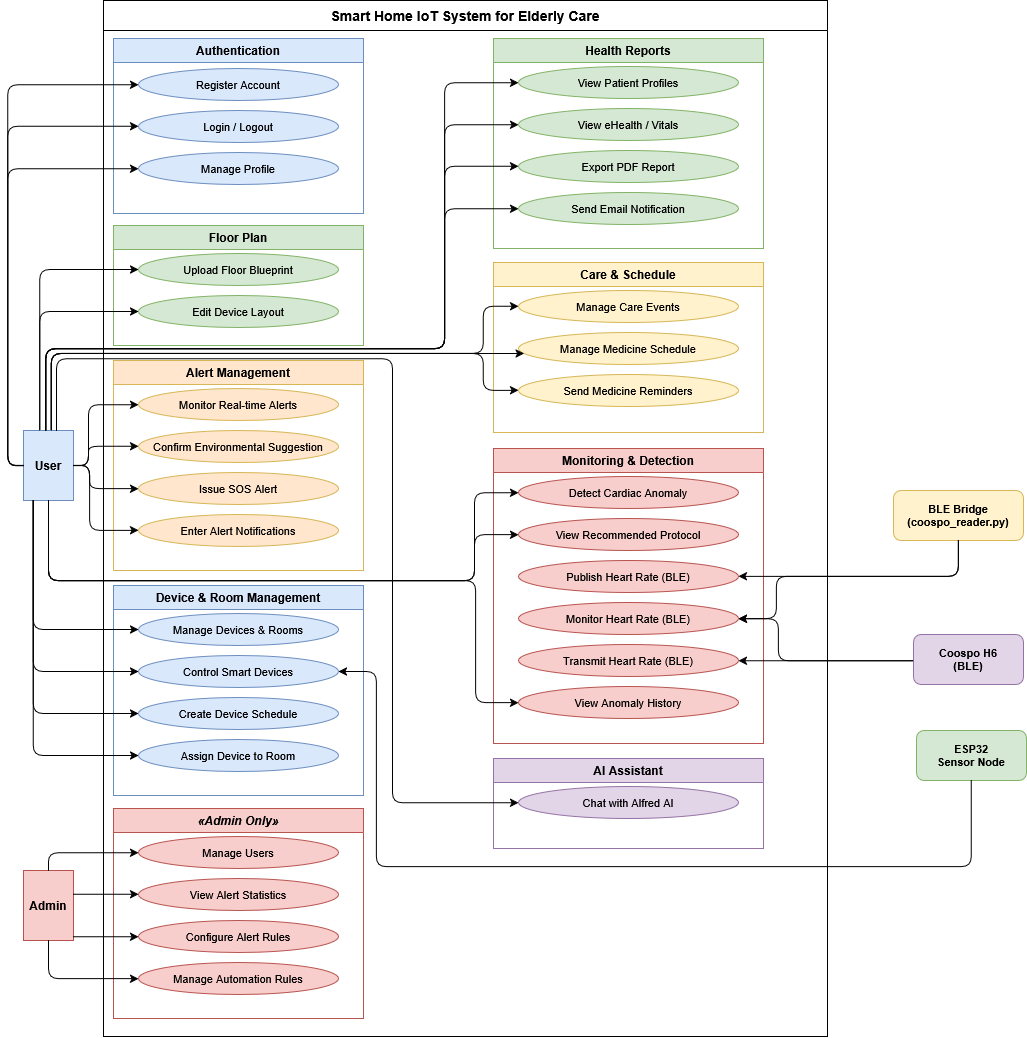
\includegraphics[width=\textwidth,height=0.92\textheight,keepaspectratio]{images/fig_usecase_diagram.png}}
\caption[UML use case diagram of the Smart Home IoT System for Elderly Care]{%
  UML use case diagram of the Smart Home IoT System for Elderly Care.
  Four actors interact with 26 use cases grouped into nine feature packages:
  \textit{User} (caregiver) accesses Authentication, Floor Plan, Alert Management,
  Device \& Room Management, Health Reports, Care \& Schedule, Monitoring \& Detection,
  and AI Assistant packages.
  \textit{Admin} inherits all User interactions via a generalisation arrow and additionally
  accesses the \textit{«Admin Only»} package (Manage Users, Configure Alert Rules,
  View Alert Statistics, Manage Automation Rules).
  \textit{ESP32 Sensor Node} and \textit{Coospo H6 (BLE)} are hardware actors that
  publish data through the Monitoring \& Detection package.}
\label{fig:usecase_diagram}
\end{figure}

% ─────────────────────────────────────────────────────────────
\section{Hardware Platform and Sensor Suite}
\label{sec:hardware_method}

\subsection{Microcontroller Selection}

The hardware node is based on the \textbf{ESP32-WROOM-32} module (Espressif Systems). The ESP32 integrates a dual-core Tensilica LX6 processor, clocked at up to 240\,MHz, along with 520\,KB of on-chip SRAM and 4\,MB of SPI Flash. Compared with the older ESP8266, the ESP32 integrates Wi-Fi (802.11\,b/g/n) and Bluetooth~4.2 (including BLE) into a single system-on-chip, making it well suited for IoT applications that require stable cloud communication while supporting nearby Bluetooth peripherals.

Key characteristics relevant to this design:

\begin{itemize}

\item \textbf{ADC}: two 12-bit SAR ADC units (18 ADC-capable channels across 34 GPIO pins);
here used to read the ambient-light LDR on GPIO 32 at 4096 discrete levels.
\item \textbf{Security engine}: hardware accelerators for AES, SHA-256,
RSA-2048, and ECC allow \texttt{WiFiClientSecure} to support TLS\,1.2
without an external cryptographic chip, enabling secure MQTT over
port~8883. On the Python backend side, the MQTT client uses
\texttt{ssl.create\_default\_context()} which verifies the broker
certificate against the system CA bundle; since EMQX Cloud provides a
certificate signed by a recognised CA, no manual CA file distribution
is required.
\item \textbf{Power}: 3.3\,V logic; an HLK-PM01 module on the PCB
converts 220\,V AC mains to a regulated 3.3\,V DC supply.
\item \textbf{Dual-core}: The ESP32 integrates two Tensilica LX6 cores.
In this firmware, all tasks (Wi-Fi keepalive, MQTT processing, sensor
acquisition, relay control, and LCD refresh) run sequentially inside the
single Arduino \texttt{loop()} on the default core, keeping the firmware
simple and avoiding inter-core synchronisation overhead.

\end{itemize}

\subsection{Sensor Suite and Actuators}

The node comprises four input sensors and two relay-based actuators.
Their key specifications are listed in Table~\ref{tab:sensor_specs}, and
the complete GPIO assignments are listed in Table~\ref{tab:pins}.

\begin{table}[H]
\centering
\caption{Sensor specifications for the ESP32 node}
\label{tab:sensor_specs}
\small
\begin{tabular}{p{3cm}p{3.5cm}p{4.5cm}p{2.5cm}}
\toprule
\textbf{Sensor} & \textbf{Interface} & \textbf{Range / Resolution} & \textbf{Notes} \\
\midrule
DHT11           & 1-Wire (GPIO\,15)    & 0--50\,$^\circ$C, $\pm2\,^\circ$C;\newline 20--80\% RH, $\pm5$\% & 5\,s publish interval \\
LDR             & ADC (GPIO\,32)       & 0--4095 raw, normalised 0--100 & 12-bit SAR ADC \\
PIR (HC-SR501)  & Digital (GPIO\,33)   & Binary: DETECTED / CLEAR       & Edge-triggered publish \\
Coospo H6       & BLE GATT\,0x2A37~\cite{BluetoothSIG2011}     & 30--240\,bpm, $\pm$1\,bpm      & Python BLE bridge \\
\bottomrule
\end{tabular}
\end{table}

\begin{table}[H]
\centering
\caption{ESP32 GPIO pin assignments}
\label{tab:pins}
\small
\begin{tabularx}{\textwidth}{@{}l c l X@{}}
\toprule
\textbf{Component} & \textbf{GPIO} & \textbf{Mode} & \textbf{Description} \\
\midrule
DHT11 & 15 & Digital input & Temperature \& humidity sensor (1-wire) \\
LDR (photoresistor) & 32 & ADC input & Ambient light, raw 0--4095, normalised 0--100 \\
PIR motion sensor & 33 & Digital input & Motion detection (edge-triggered) \\
Relay 1 (\texttt{den}) & 17 & Digital output & Light relay (active-high) \\
Relay 2 (\texttt{quat}) & 16 & Digital output & Fan relay (active-high)$^\dagger$ \\
I2C SDA (LCD) & 21 & I2C data & 16x2 LCD backpack data line \\
I2C SCL (LCD) & 22 & I2C clock & 16x2 LCD backpack clock line \\
Button 1 & 0 & Digital input & Physical toggle for Relay 1 \\
Button 2 & 2 & Digital input & Physical toggle for Relay 2$^\dagger$ \\
\bottomrule
\multicolumn{4}{@{}p{\textwidth}@{}}{\footnotesize $^\dagger$ P2 connector (Button~2 / Relay~2) damaged during testing; physical button non-functional but MQTT software control remains operational.} \\
\end{tabularx}
\end{table}

The DHT11 was selected over the more accurate DHT22 ($\pm0.5\,^\circ$C) and SHT31 ($\pm0.3\,^\circ$C) due to its lower cost and availability, making it suitable for a prototype. Its $\pm2\,^\circ$C tolerance is sufficient since temperature is used as \textit{contextual} input to the anomaly pipeline, not a clinical measurement (see Section~\ref{sec:future}).

Due to Wi-Fi/BLE coexistence constraints on the ESP32, the heart-rate acquisition from the \textbf{Coospo H6} chest strap (Figure~\ref{fig:coospo_h6}) is offloaded to a Python service that reads BPM via BLE GATT~\cite{BluetoothSIG2011} and forwards it at $\sim$1\,Hz to the MQTT topic \texttt{home/sensors/heart\_rate}. If disconnected, the service retries with a linear back-off ($\min(5 \times \mathit{retry},\,30)$\,s) and re-subscribes by MAC address. Gaps during outages are not buffered and appear as missing segments in the BPM chart, which is noted as a hardware limitation in Section~\ref{sec:future}.


\begin{figure}[H]
\centering
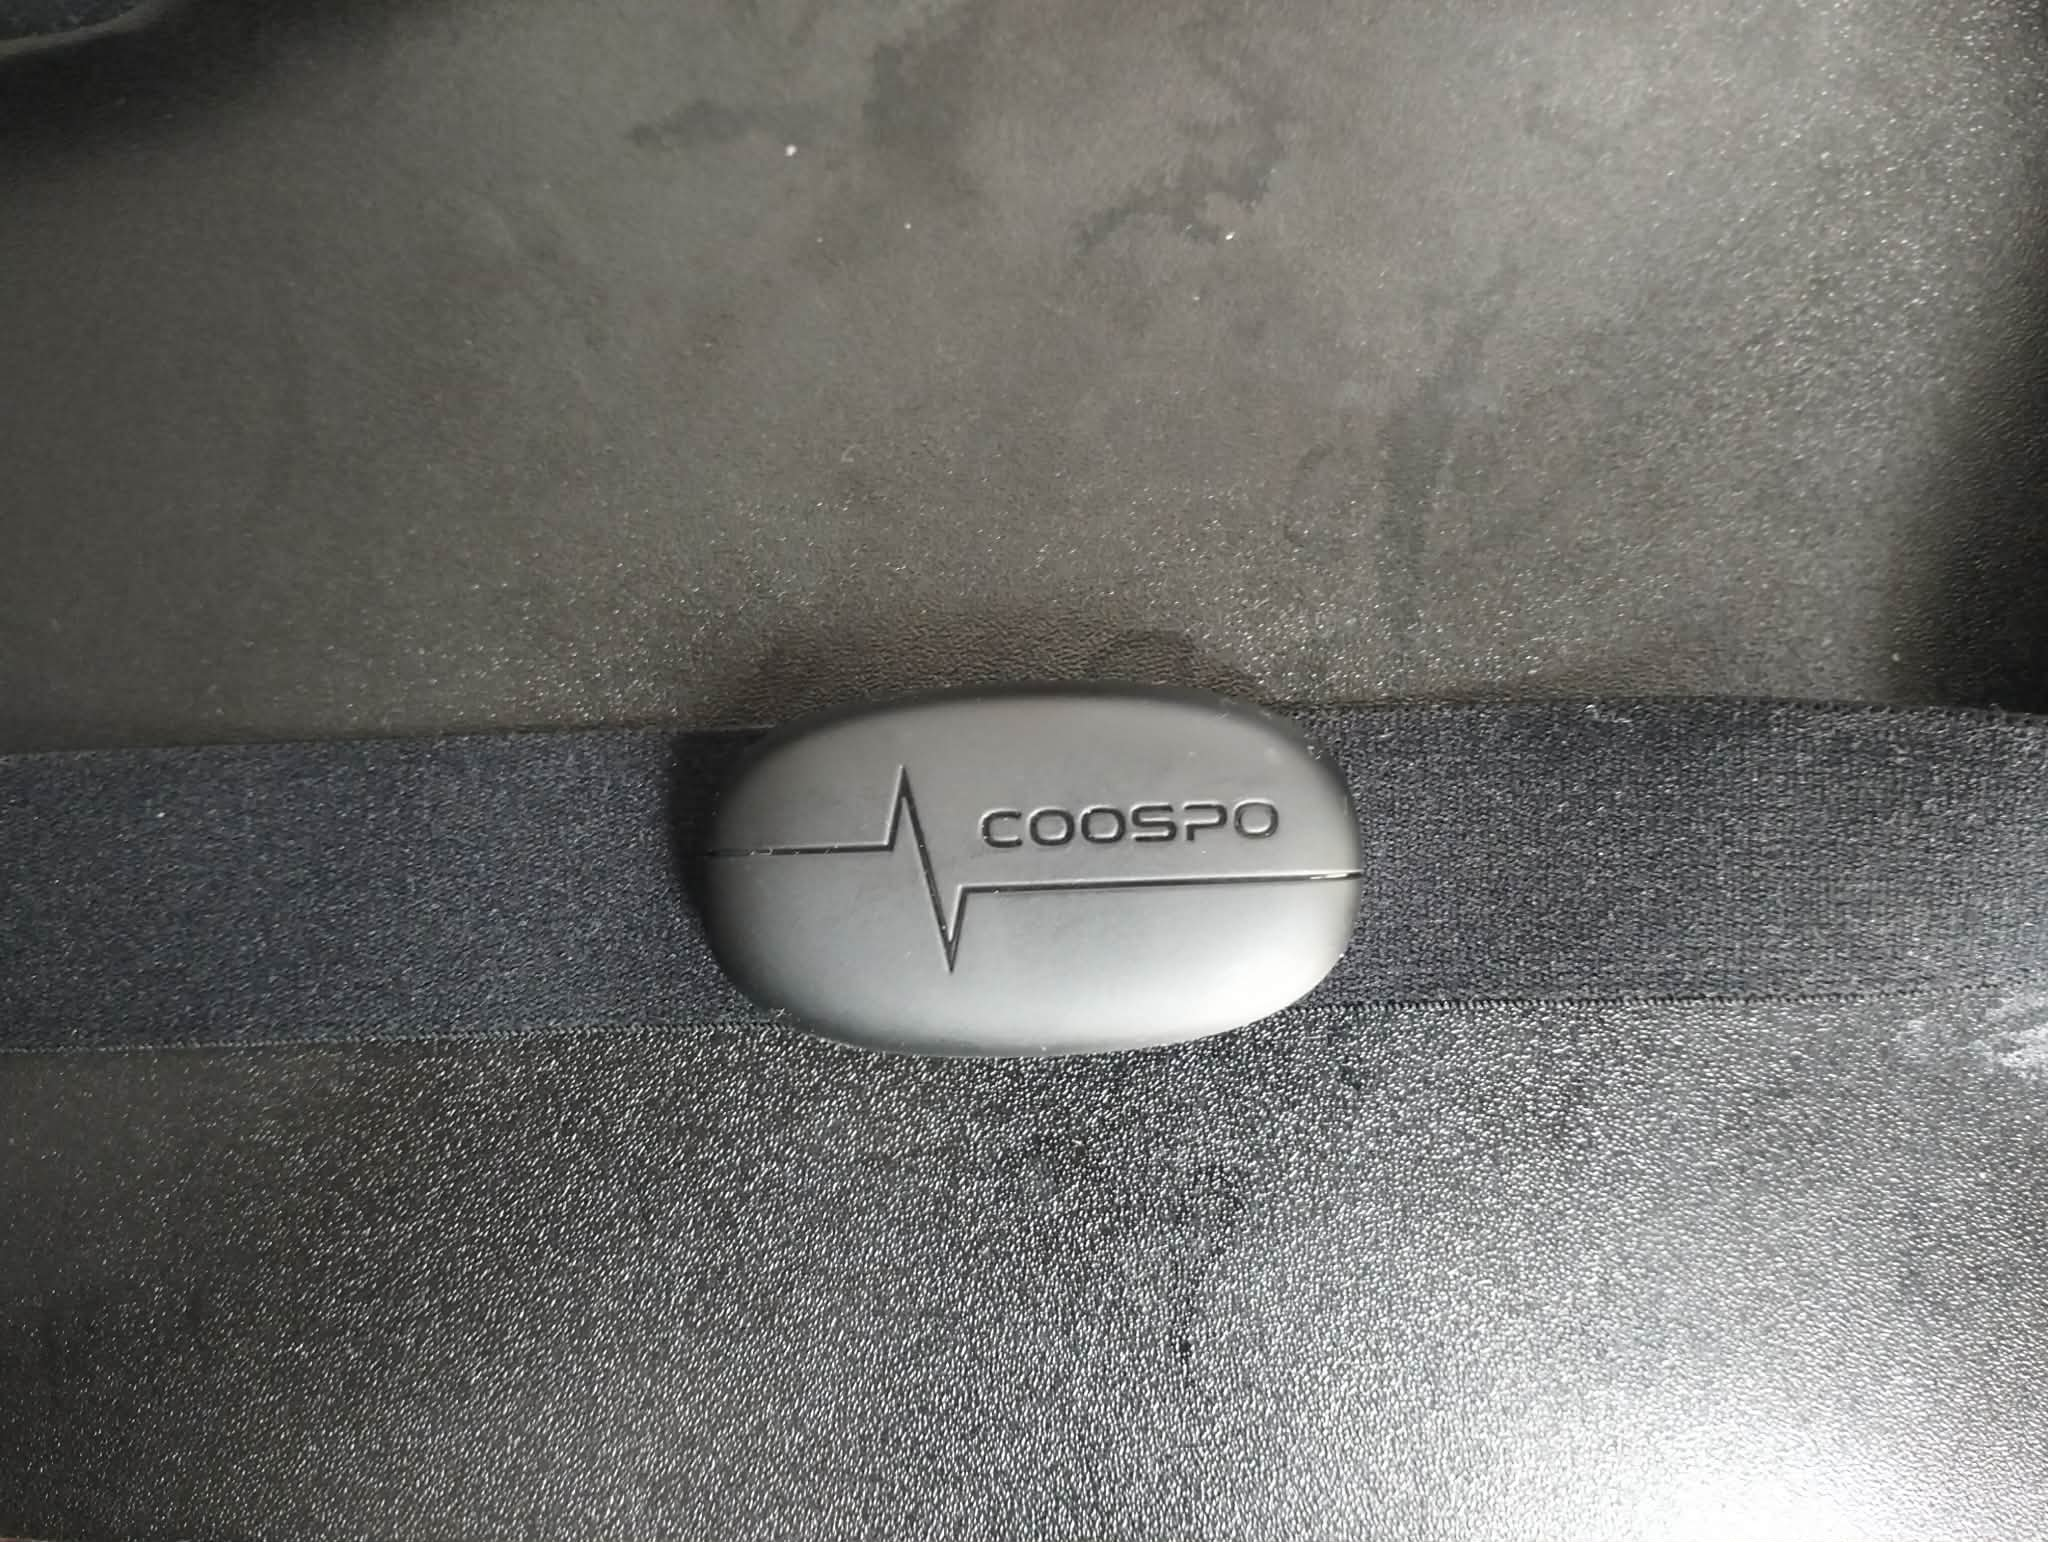
\includegraphics[width=0.50\textwidth]{images/coospo_h6.png}
\caption[Coospo H6 BLE heart-rate monitor]{Coospo H6 BLE chest-strap heart-rate monitor (GATT 0x2A37, $\sim$1\,Hz).}
\label{fig:coospo_h6}
\end{figure}

\subsection{Hardware Platform (PCB)}

The breadboard prototype was replaced by an ESP32 node on a two-layer PCB which contains the ESP32 module, relay driver circuits (2N3904 NPN transistors and 1N4007 flyback diodes), an HLK-PM01 AC/DC power supply, sensor connectors and touch-button inputs as a single assembly. This board is from previous hardware coursework and is reused in this thesis as the physical platform for the node. As such, the contribution of this thesis at the hardware layer is the firmware, sensor integration and BLE bridge, not the board design itself.
For completeness, Figure~\ref{fig:pcb_all} presents the schematic, the routed layout and 3D render of the board.

\begin{figure}[htbp]
  \centering
  \begin{subfigure}[b]{0.48\textwidth}
    \centering
    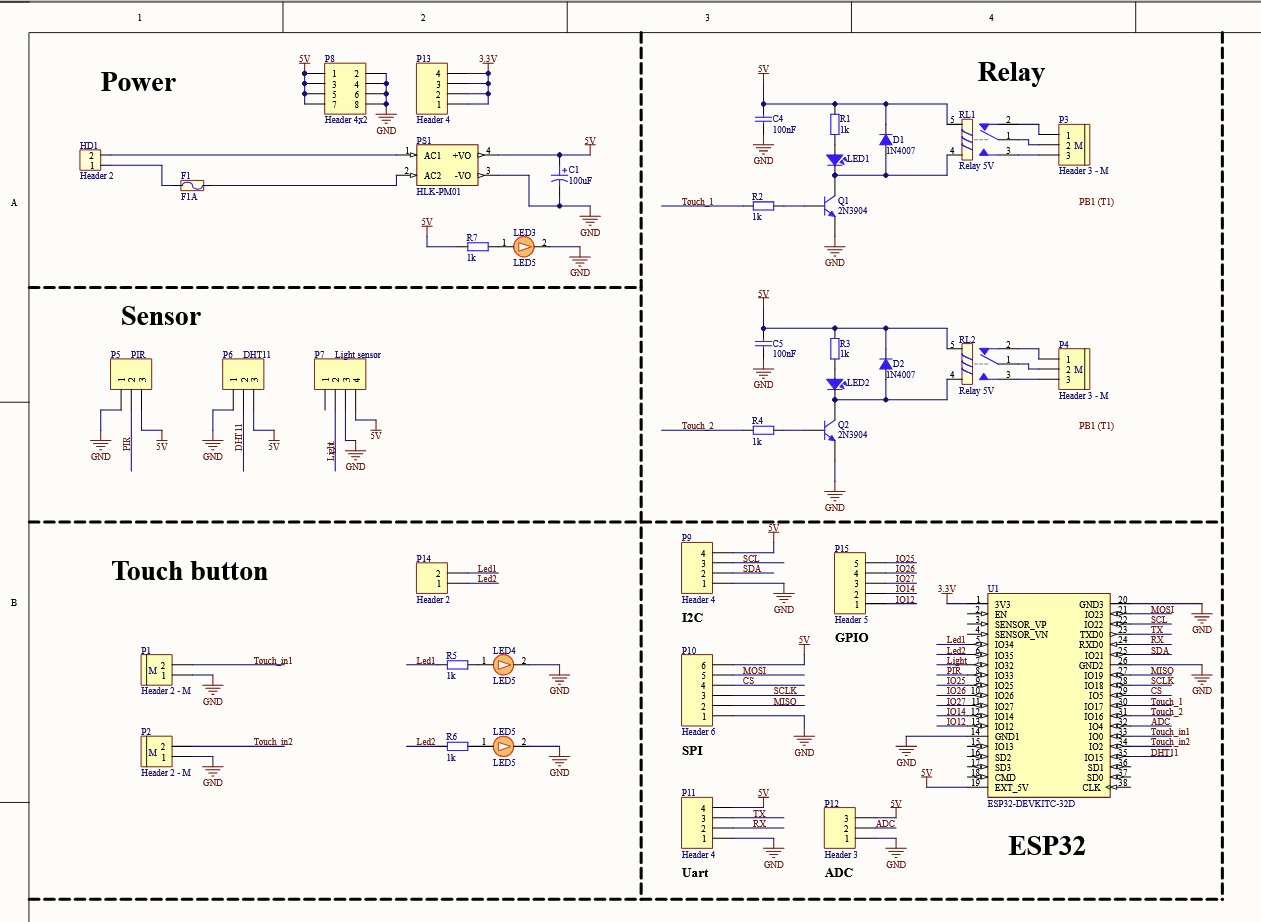
\includegraphics[width=\textwidth]{images/pcb_schematic.png}
    \caption{PCB schematic}
    \label{fig:pcb_schematic}
  \end{subfigure}
  \hfill
  \begin{subfigure}[b]{0.48\textwidth}
    \centering
    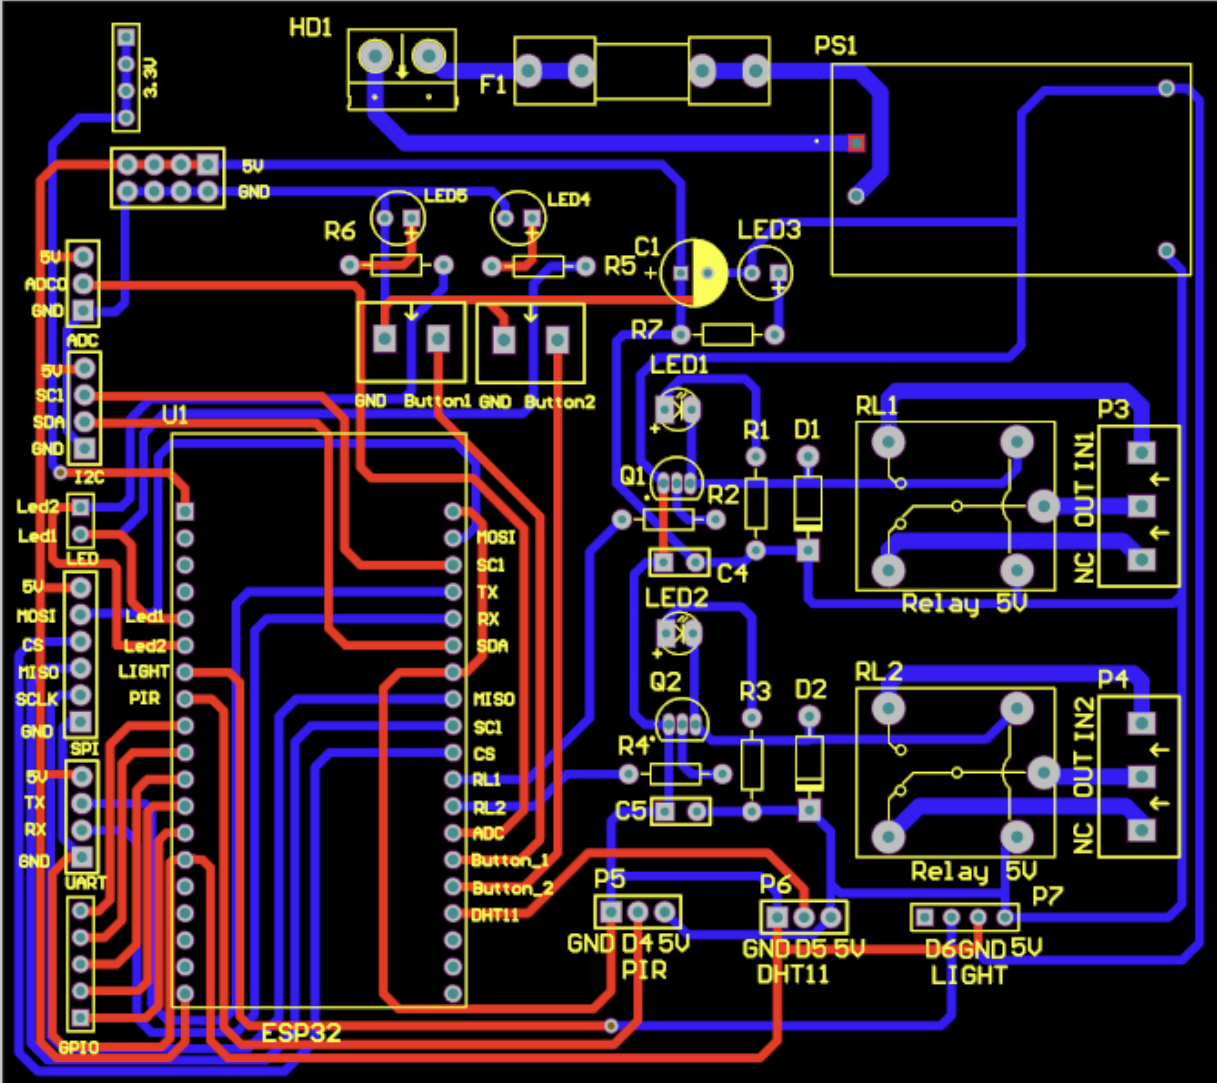
\includegraphics[width=\textwidth]{images/pcb_layout.png}
    \caption{Routed PCB layout (two-layer)}
    \label{fig:pcb_layout}
  \end{subfigure}
  \vspace{0.5em}
  \begin{subfigure}[b]{0.6\textwidth}
    \centering
    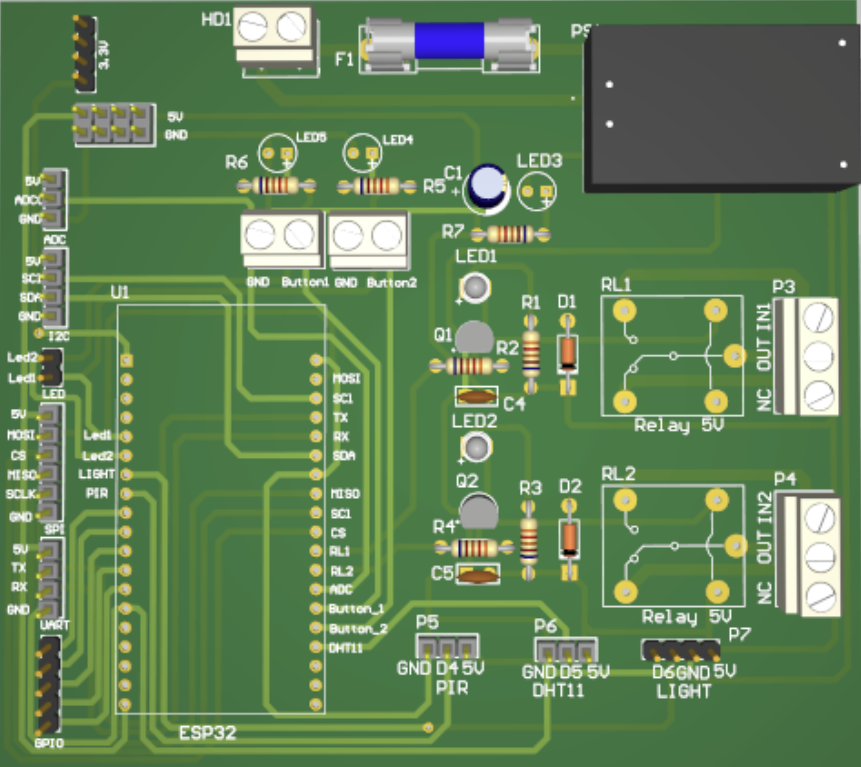
\includegraphics[width=\textwidth]{images/pcb_3d.png}
    \caption{3D render of the assembled PCB}
    \label{fig:pcb_3d}
  \end{subfigure}
  \caption[Two-layer PCB hardware platform]{Two-layer PCB used as the hardware platform (from prior coursework).}
  \label{fig:pcb_all}
\end{figure}

\FloatBarrier

% ─────────────────────────────────────────────────────────────
\section{Data Acquisition and Preprocessing}
\label{sec:data_method}

\subsection{Sensor Data Flow}

Environmental sensors (DHT11, LDR, PIR) publish readings every five seconds to the EMQX Cloud MQTT broker over TLS. Heart-rate data from the Coospo~H6 is streamed via the Python BLE bridge at approximately 1\,Hz. All messages are delivered to the Flask backend through wildcard subscriptions.
(\texttt{home/sensors/\#}~and~\texttt{home/status/\#}), parsed, and persisted
to MySQL through the SQLAlchemy ORM.

\subsection{Preprocessing Pipeline}

Before being fed into the machine learning pipeline, the data goes through the following steps:
    \begin{enumerate}
    \item \textbf{LDR normalisation}: the 12-bit ADC raw value (0--4095) is mapped to a 0--100 light intensity scale.
    \item \textbf{PIR edge filtering}: record only state-change events (DETECTED~$\leftrightarrow$~CLEAR) to prevent duplicate entries.
    \item \textbf{Heart-rate throttling}: a per-user 60-second write throttle, protected by a \texttt{threading.Lock}, ensures no concurrent database writes during continuous BPM streaming.
    \item \textbf{Temporal feature derivation}: from each UTC server
    timestamp the system derives \texttt{hour} (0--23), \texttt{is\_night}
    ($= 1$ if $20 \leq \text{hour}$ or $\text{hour} \leq 6$), and
    \texttt{is\_dark} ($= 1$ if light\_level $< 50$), providing circadian
    and environmental context to the anomaly pipeline.
    \item \textbf{Feature standardisation}: heart-rate values are normalised
    using a dedicated \texttt{StandardScaler}
    (\texttt{anomaly\_hr\_scaler.pkl}) before Isolation Forest inference.
\end{enumerate}

% ─────────────────────────────────────────────────────────────
\section{Technology Selection and Design Decisions}
\label{sec:tech_selection}

This section summarizes the major technology decisions that define the platform and the rationale for them, so that the designs for each component in the following sections can be read against a single set of decisions. The selection of each component is motivated by the elderly-care requirements (Section~\ref{sec:user_req}), i.e. low cost, low power, real-time responsiveness, data privacy and an accessible bilingual interface, and the gaps identified in the literature review. In Table~\ref{tab:tech_decisions}, the selected technologies, the main alternatives considered and the deciding rationale are summarized. The most consequential choices are elaborated in the remainder of this chapter.

\begin{table}[p]
\centering
\caption[Technology selections and design decisions]{Summary of technology selections and design decisions}
\label{tab:tech_decisions}
\footnotesize
\renewcommand{\arraystretch}{1.05}
\setlength{\tabcolsep}{4pt}
\begin{tabularx}{\textwidth}{@{} >{\raggedright\arraybackslash}p{2.5cm} >{\raggedright\arraybackslash}p{3.0cm} >{\raggedright\arraybackslash}p{2.6cm} >{\raggedright\arraybackslash}X @{}}
\toprule
\textbf{Concern} & \textbf{Selected} & \textbf{Alternatives} & \textbf{Deciding rationale} \\
\midrule
Microcontroller & ESP32-WROOM-32 & Arduino Uno, Raspberry Pi &
  \begin{tblitem}
    \item Dual-core with integrated Wi-Fi and BLE.
    \item Low unit cost and power draw.
    \item Sufficient GPIO headroom for sensor sampling and TLS MQTT.
  \end{tblitem} \\
\addlinespace[4pt]
Device messaging & MQTT over TLS & HTTP polling, CoAP &
  \begin{tblitem}
    \item Lightweight publish/subscribe, low overhead on constrained devices.
    \item Broker-mediated decoupling between sensor nodes and the backend.
  \end{tblitem} \\
\addlinespace[4pt]
Wearable HR link & Bluetooth Low Energy & Classic Bluetooth, ANT+ &
  \begin{tblitem}
    \item Low-power Heart Rate Service profile.
    \item Natively supported by ESP32 and host laptop; ANT+ requires a proprietary USB receiver.
  \end{tblitem} \\
\addlinespace[4pt]
Backend framework & Flask & FastAPI, Django &
  \begin{tblitem}
    \item Lightweight WSGI Python framework.
    \item FastAPI's async model conflicts with Flask-SocketIO threading and synchronous SQLAlchemy.
  \end{tblitem} \\
\addlinespace[4pt]
Backend structure & Modular layered & Monolithic MVC &
  \begin{tblitem}
    \item Separates domain, use-case, AI, gateway, infrastructure, and presentation concerns into distinct packages.
    \item Enables independent testing and replacement of individual components (Section~\ref{sec:arch_method}).
  \end{tblitem} \\
\addlinespace[4pt]
Web dashboard & Vite + Vanilla JS & React, Vue &
  \begin{tblitem}
    \item Direct control of the interactive floor-plan rendering without the overhead of a heavier SPA framework.
  \end{tblitem} \\
\addlinespace[4pt]
Mobile application & Flutter & React Native, native &
  \begin{tblitem}
    \item Single Dart codebase targeting both Android and iOS with a consistent user experience; the build was validated on Android in this work.
  \end{tblitem} \\
\addlinespace[4pt]
Anomaly detection & Isolation Forest (heart-rate only) & One-Class SVM, autoencoders, fixed threshold &
  \begin{tblitem}
    \item Unsupervised one-class model; no labelled anomalies required.
    \item Full algorithm comparison in Section~\ref{subsec:ml_selection}.
    \item Sub-millisecond inference confirmed in Section~\ref{subsec:latency_protocol}.
  \end{tblitem} \\
\addlinespace[4pt]
Conversational AI & Tri-modal: Rule, Ollama qwen2.5:3b, Gemini & Cloud-only LLM &
  \begin{tblitem}
    \item Local rule and on-device LLM paths preserve privacy and enable offline fallback.
    \item Cloud path (Gemini Flash) adds open-ended capability (Section~\ref{sec:alfred_method}).
  \end{tblitem} \\
\bottomrule
\end{tabularx}
\end{table}
% ─────────────────────────────────────────────────────────────
\section{System Architecture Design}
\label{sec:arch_method}

\subsection{Four-Tier Architecture and Physical Deployment}
\label{subsec:deployment}

The platform uses a four-tier IoT architecture, with communication
following a unidirectional data flow from the hardware layer upward to the
presentation layer:

\begin{itemize}
    \item \textbf{Hardware layer.} The ESP32 node collects environmental and physiological signals and controls relay actuators. A Python BLE bridge handles heart-rate data from the Coospo H6 wearable.

    \item \textbf{Communication layer.} An EMQX Cloud MQTT broker acts as the main message hub. All sensor telemetry and device-control commands are transmitted over TLS-secured connections.

    \item \textbf{Backend layer.} A Python Flask service receives incoming sensor data, stores it in MySQL, runs the anomaly detection pipeline, exposes REST endpoints and Socket.IO events, while also hosting the Alfred AI assistant.

    \item \textbf{Presentation layer.} A Vite-based web dashboard and a Flutter mobile app form the caregiver-facing front end for monitoring, device control, health data review, and natural-language interaction.\end{itemize}

Figure~\ref{fig:deployment} shows how these four logical tiers map onto the
physical nodes of the prototype deployment. All \emph{software} services
(Flask, MySQL, Ollama, BLE bridge) run on a single developer laptop
(Windows, 16\,GB RAM). The ESP32 node and Coospo~H6 are physical hardware
devices on the local network; EMQX Cloud and Google Gemini are the primary
external cloud dependencies.

\begin{landscape}
\begin{figure}[p]
\centering
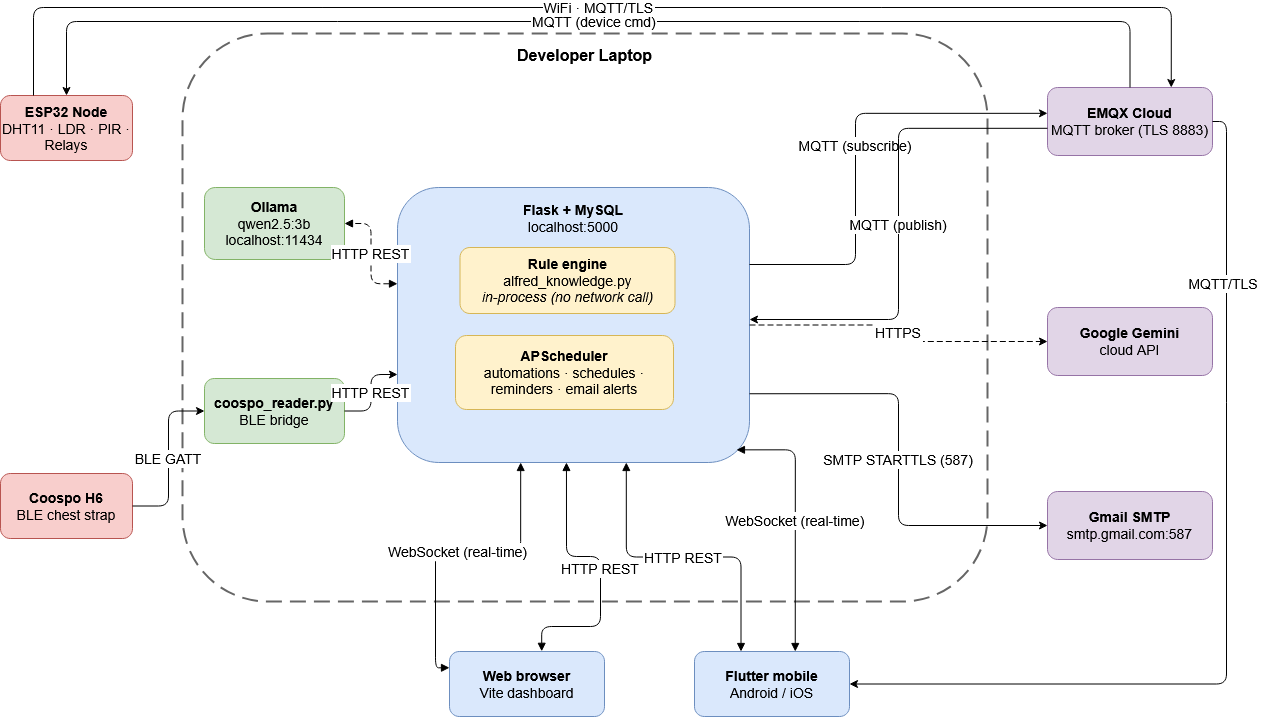
\includegraphics[width=\linewidth,height=0.80\textwidth,keepaspectratio]{images/deployment.png}
\caption[Physical deployment and four-level IoT architecture]
{Four-level IoT architecture and physical deployment. The Flask services are running on the developer laptop, and the ESP32 node and Coospo~H6 are physical devices on the local network. The Rule Engine is in-process and runs inside Flask. Ollama and Gemini are conditionally used based on Alfred mode. Optional communication paths are indicated by dashed arrows. The primary external cloud services are EMQX Cloud and Google Gemini.}
\label{fig:deployment}
\end{figure}
\end{landscape}

\FloatBarrier

\subsection{Backend Modular Structure}

The Flask backend is organised into six functional modules, each responsible for a distinct concern. Dependency injection is managed in \texttt{app/wiring.py} using a \texttt{dependency\_injector} container that wires components together at startup.

\begin{itemize}[itemsep=4pt, parsep=0pt, topsep=4pt]

    \item \textbf{Domain} (\texttt{app/domain/}): Core data models (\texttt{Device}, \texttt{Status}, \texttt{Log}) and abstract port interfaces (\texttt{publisher}, \texttt{email\_notifier}, \texttt{realtime}). No framework imports.

    \item \textbf{Use Cases} (\texttt{app/usecases/}): Orchestration of business logic --- \texttt{DeviceUseCase}, \texttt{AlertUseCase}, \texttt{AIUseCase}, and others --- coordinating between repositories, gateways, and AI services.

    \item \textbf{AI / ML} (\texttt{app/ai/}): Isolation Forest anomaly detection, mood prediction, HRV analysis, and feature engineering. The heart-rate coordination service (\texttt{heart\_rate\_ai.py}) is the central pipeline that integrates inference results with persistence, real-time notification, and alert dispatch.

    \item \textbf{Gateways} (\texttt{app/gateways/}): Protocol adapters that connect external communication channels to the application --- MQTT publisher/listener, Socket.IO emitter, and email notifier.

    \item \textbf{Infrastructure} (\texttt{app/infrastructure/}): SQLAlchemy ORM models and MySQL repository implementations providing persistence for all entities.

    \item \textbf{Presentation} (\texttt{app/presentation/api/}): Flask blueprints exposing REST endpoints and Socket.IO events to the web dashboard and mobile app.

\end{itemize}

Figure~\ref{fig:clean_arch} illustrates the module hierarchy from the most protocol-facing layer (Presentation) down to the framework-independent Domain.

\begin{figure}[H]
\centering
\begin{tikzpicture}[
  layer/.style={draw, minimum width=#1, minimum height=0.7cm,
                align=center, font=\small, rounded corners=3pt},
  lbl/.style={font=\scriptsize, align=left},
]
\def\w{9.2cm}
\node[layer=\w, fill=gray!10]     (pres) at (0, 0)    {Presentation layer \quad \texttt{app/presentation/api/} (Flask blueprints)};
\node[layer=7.8cm, fill=blue!7]   (infra)at (0,-0.85) {Infrastructure \quad \texttt{app/infrastructure/} (SQLAlchemy repos)};
\node[layer=6.4cm, fill=blue!7]   (gw)   at (0,-1.70) {Gateways \quad \texttt{app/gateways/} (MQTT, Socket.IO, email)};
\node[layer=5.0cm, fill=green!8]  (uc)   at (0,-2.55) {Use Cases \quad \texttt{app/usecases/}};
\node[layer=3.6cm, fill=orange!7] (ai)   at (0,-3.40) {AI / ML \quad \texttt{app/ai/} (anomaly detection, mood prediction)};
\node[layer=2.2cm, fill=teal!10]  (dom)  at (0,-4.25) {Domain \quad \texttt{app/domain/}};
\end{tikzpicture}
\caption[Flask backend module hierarchy]{Flask backend module hierarchy. Modules are grouped by responsibility from the protocol-facing Presentation layer down to the framework-independent Domain. The AI/ML module handles the full heart-rate processing pipeline including inference, persistence, and real-time alerting.}
\label{fig:clean_arch}
\end{figure}

\FloatBarrier

\subsection{Database Schema Design}

The system uses MySQL~8.0, managed by SQLAlchemy, and is divided into three entity modules: Auth, Health, and Device. Table~\ref{tab:db} summarises the
core tables; the complete entity-relationship diagram is presented in
Figure~\ref{fig:erd_full}.

\begin{table}[H]
\centering
\caption{Core database tables grouped by module}
\label{tab:db}
\small
\begin{tabularx}{\textwidth}{@{} l >{\RaggedRight\arraybackslash}X @{}}
\toprule
\textbf{Module / Table} & \textbf{Purpose} \\
\midrule
\multicolumn{2}{@{}l}{\textit{Auth module}} \\
\quad\texttt{users}                    & Accounts, hashed passwords, role (\texttt{admin}/\texttt{user}/\texttt{guest}) \\
\quad\texttt{password\_reset\_tokens}  & Time-limited reset codes (hashed, 30-min expiry) \\
\quad\texttt{alert\_mute\_preferences} & Per-user alert visibility mute scope and keyword \\
\quad\texttt{alert\_saved\_view\_configs} & Persisted alert filter presets (level, device, date range) per user \\
\midrule
\multicolumn{2}{@{}l}{\textit{Health module}} \\
\quad\texttt{patient\_profiles}   & Name, age, gender, baseline HR, diagnosis notes, medications \\
\quad\texttt{patient\_hr\_records}& BPM, severity, risk level, mood label \\
\quad\texttt{medicine\_reminders} & Medicine name, dosage, time, recurrence pattern, active flag \\
\midrule
\multicolumn{2}{@{}l}{\textit{Device module}} \\
\quad\texttt{rooms}         & Room name, polygon JSON, floor-plan URL \\
\quad\texttt{device}        & Device code, category, room assignment, map coordinates \\
\quad\texttt{device\_status}& Latest ON/OFF state and value per device \\
\quad\texttt{sensor\_data}  & Time-series sensor readings \\
\quad\texttt{control\_log}  & Audit trail of all device commands \\
\quad\texttt{alerts}        & Anomaly events with severity and read state \\
\quad\texttt{notifications} & Per-user in-app notification records (title, body, read state) linked to an alert \\
\quad\texttt{alert\_rules}  & Threshold rules per device/sensor type \\
\quad\texttt{schedules}     & Cron-based scheduled device actions \\
\quad\texttt{automations}   & Trigger-action pairs for conditional automation \\
\bottomrule
\end{tabularx}
\end{table}

The alert-visibility mute feature is persisted in the dedicated \texttt{alert\_mute\_preferences} table, and the backend restores the saved scope and keyword when the user comes back on another device. A dedicated repair script \texttt{backend/migrate\_alert\_mute\_preferences.py} creates the table if it does not exist, and safely adds the required columns and indexes if the schema is incomplete.

\begin{landscape}
\begin{figure}[p]
\centering
% In an lscape landscape page the visual height corresponds to \textwidth.
% Cap the image well below \textwidth so the multi-line caption also fits
% on the same rotated page.
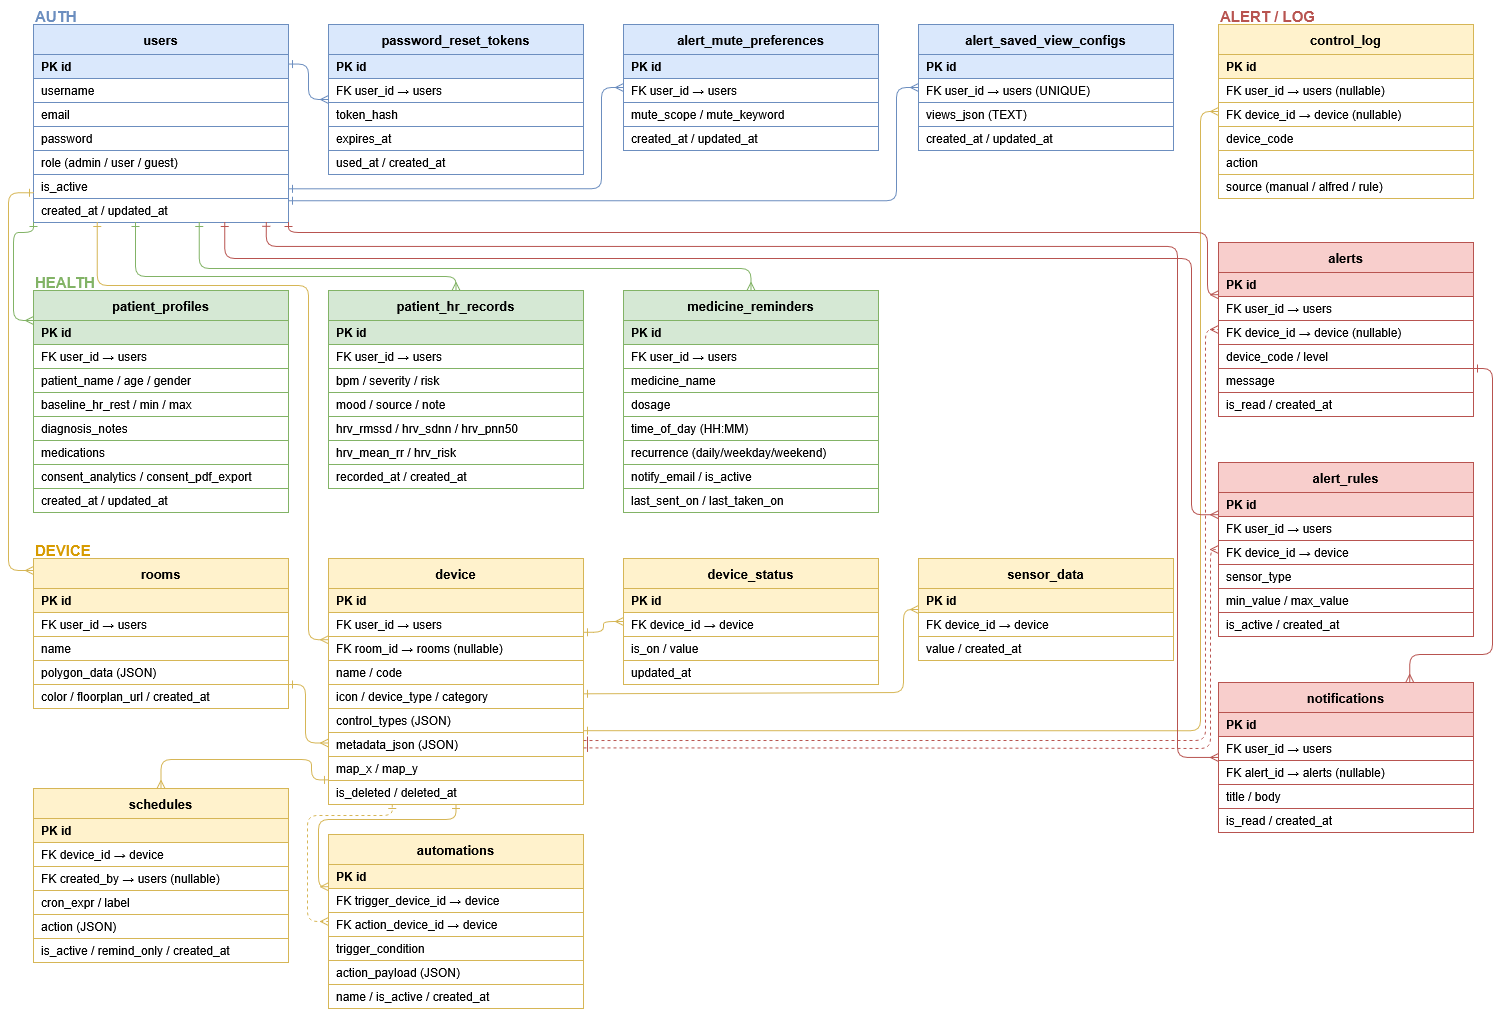
\includegraphics[width=\linewidth,height=0.80\textwidth,keepaspectratio]{images/erd_full.png}
\caption[Database entity-relationship diagram]{Complete database schema (17
  tables). \emph{Auth}: \texttt{users}, \texttt{password\_reset\_tokens},
  \texttt{alert\_mute\_preferences}, \texttt{alert\_saved\_view\_configs}.
  \emph{Health}: \texttt{patient\_profiles}, \texttt{patient\_hr\_records},
  \texttt{medicine\_reminders}. \emph{Device Core}: \texttt{rooms},
  \texttt{device}, \texttt{device\_status}, \texttt{sensor\_data},
  \texttt{control\_log}. \emph{Device Events}: \texttt{alerts},
  \texttt{alert\_rules}, \texttt{notifications}, \texttt{schedules},
  \texttt{automations}.}
\label{fig:erd_full}
\end{figure}
\end{landscape}


\subsection{Authentication and Role-Based Access Control}
\label{subsec:rbac}

The platform defines two active roles: \texttt{admin} and \texttt{user} (the default). A \texttt{guest} role exists in the schema for future caregiver-observer workflows but is not yet activated. Admins can configure accounts, assign automation rules --- for example, triggering a fan when temperature exceeds 40\,°C --- and act on behalf of any patient. Regular users see only their own sensor data, alerts, schedules, and AI outputs.

Tokens are signed with \texttt{itsdangerous.URLSafeTimedSerializer} on a 7-day TTL and verified without a database round-trip: the \texttt{@auth\_required} decorator checks the signature and loads \texttt{g.current\_user} straight from the token payload. How the token travels depends on the client. The web dashboard keeps it in an \texttt{HttpOnly} cookie (\texttt{SameSite=Strict}) so JavaScript cannot read it; the Flutter app sends it as a \texttt{Bearer} header on every request, since Dart's HTTP layer has no cookie jar. A separate \texttt{@admin\_required} decorator guards any endpoint that regular users should not reach and returns \texttt{403} on a role mismatch.

Data isolation is enforced at three levels. Every ORM query filters by \texttt{user\_id}. Route handlers re-verify ownership before returning a resource and respond with \texttt{404} rather than \texttt{403} so that the existence of another user's record is not leaked. Real-time events are confined to per-user Socket.IO rooms (\texttt{user\_\{id\}}), so a patient's sensor alerts and AI replies never cross into another active session.

\clearpage

% ─────────────────────────────────────────────────────────────
\section{User Interface Design}
\label{sec:ui_method}

\subsection{Web Dashboard Layout}

The web dashboard is a single page application (Vite/ES6 modules). It is divided into 7 pages, with a persistent sidebar (the Admin page is hidden for non-admin users):
\begin{itemize}[itemsep=4pt, parsep=0pt, topsep=4pt]
    \item \textbf{Dashboard}: A unified home view that brings together key patient and system information, including real-time vital signs, weather updates, schedule overview, active alerts, and AI-based health insights generated by Alfred, along with quick access to device controls.

    \item \textbf{Health Monitor}: A real-time monitoring interface for visualizing heart rate trends, anomaly risk flags, and AI-generated mood labels retrieved from the backend via Socket.IO and REST endpoints.

    \item \textbf{Floor-Plan Editor}: A visual editor that allows caregivers to define room layouts from uploaded floor-plan images by drawing room boundaries, assigning devices, and managing multiple floors.

    \item \textbf{Alert Management}: A centralized system for tracking and managing alerts with severity-based filtering and user-defined mute rules. Critical events, including SOS alerts triggered by detected distress signals from the AI system, are recorded and automatically sent to caregivers.

    \item \textbf{Care and Schedule}: A calendar-based module for managing daily activities, medications, and device automation. It supports multiple views and allows caregivers to define time-based actions using cron-like scheduling.

    \item \textbf{Health Report}: A reporting module that generates daily and weekly summaries of patient status, including vital signs, alert history, medication adherence, and AI analysis, with support for export via print or email.

    \item \textbf{Admin} (role-gated): A restricted area for managing caregiver accounts, assigning patients, and handling role-based access control.
\end{itemize}

Figure~\ref{fig:method_dashboard_layout} depicts the main Dashboard , and screenshots of the remaining views are presented in Chapter~4.

\begin{figure}[htbp]
\centering
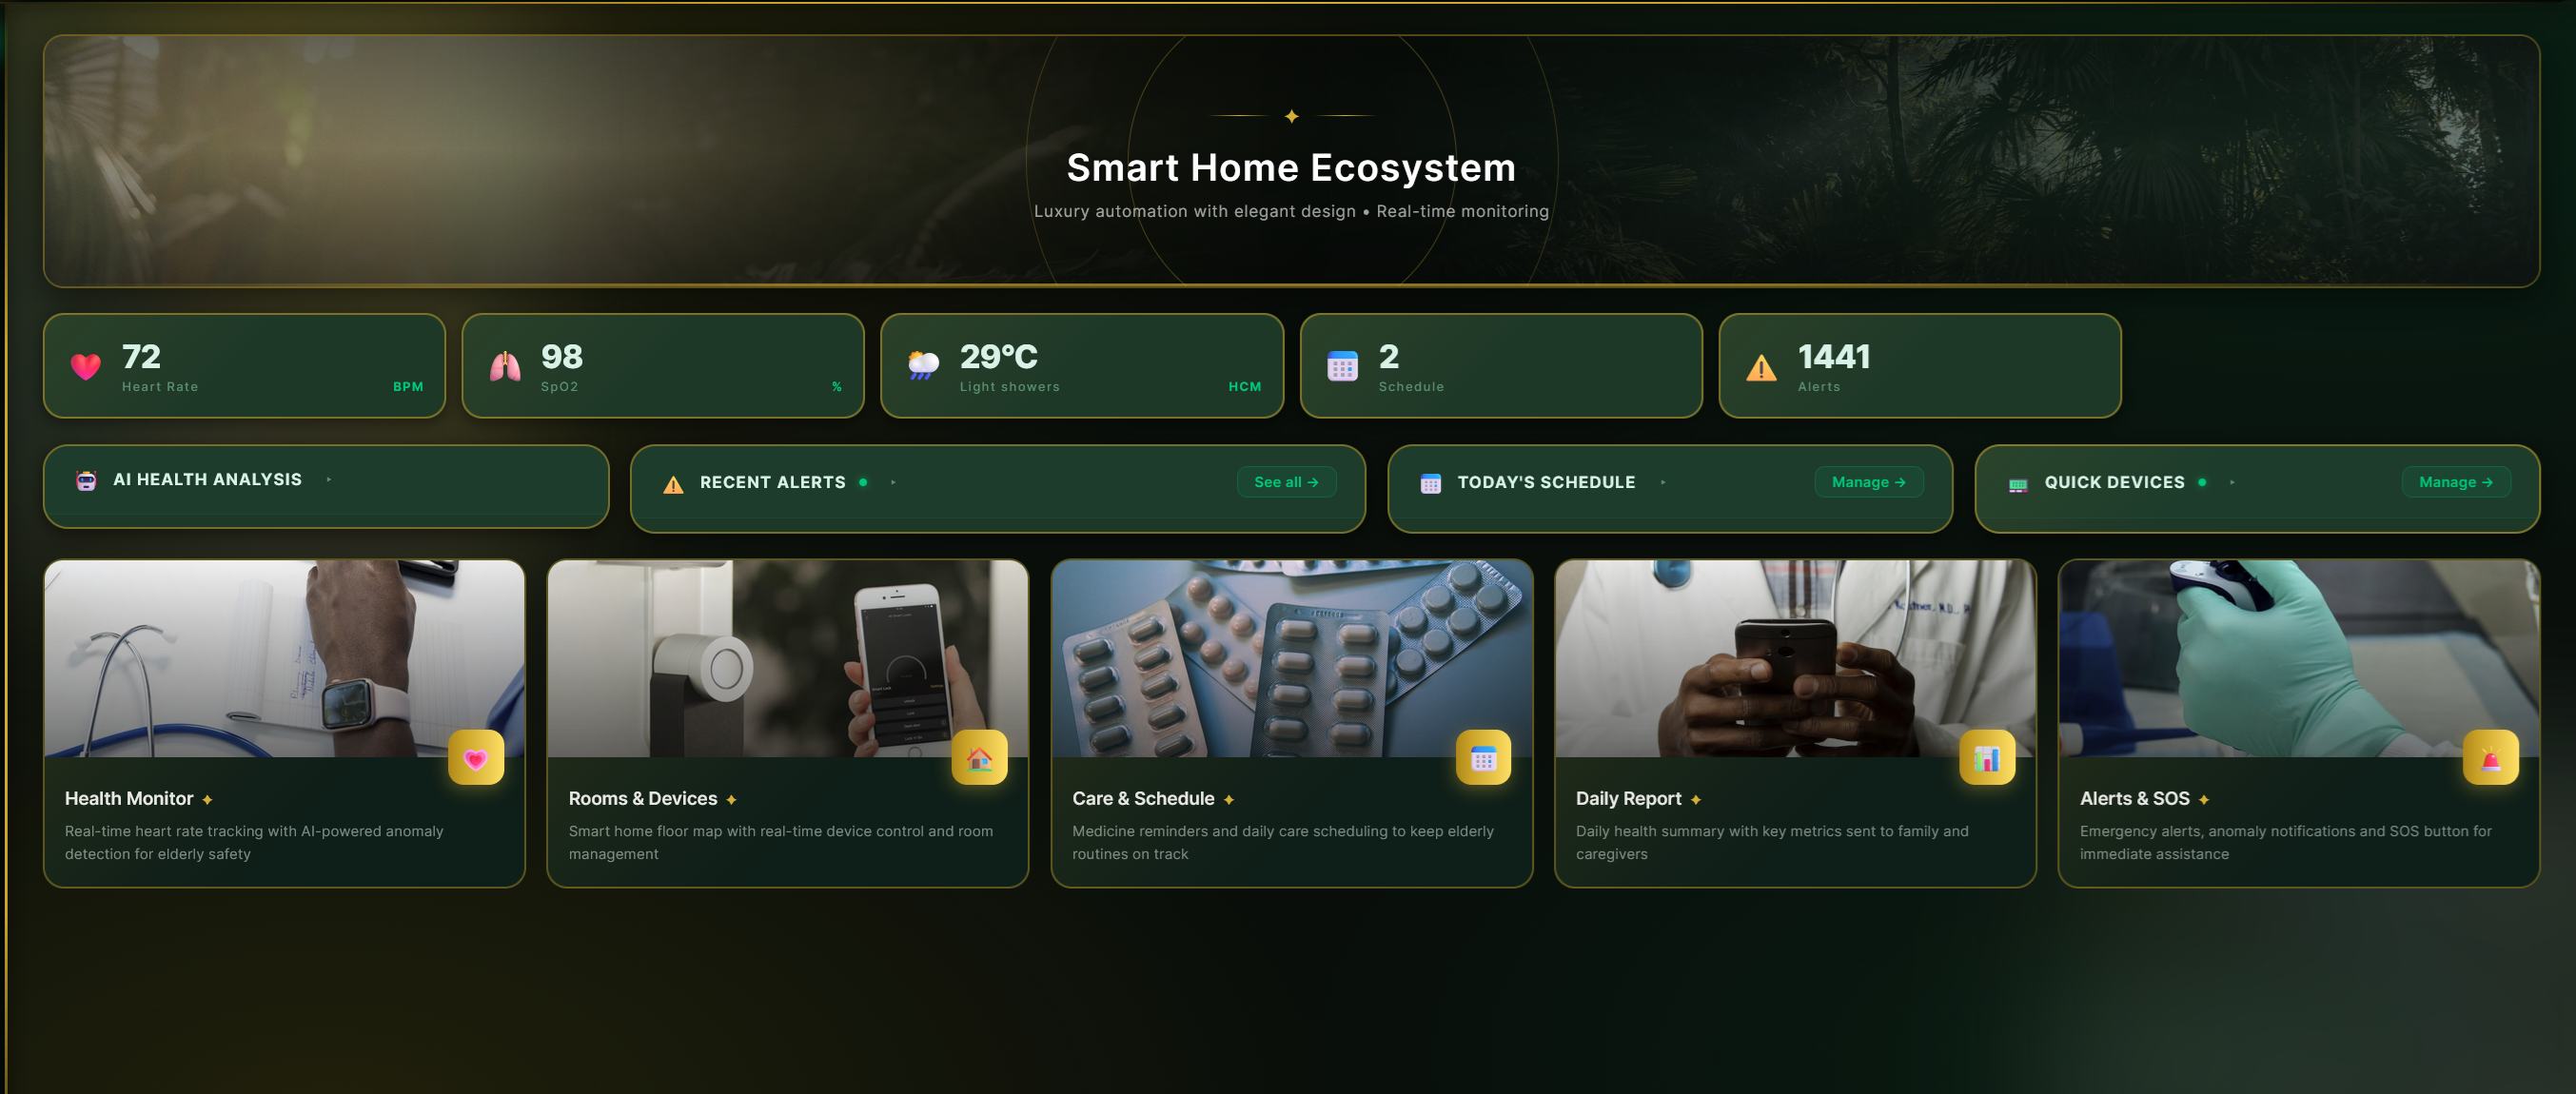
\includegraphics[width=0.92\textwidth]{images/web_dashboard.png}
\caption[Web dashboard layout]{Web dashboard layout showing the live sensor tiles, real-time
  heart-rate chart, device toggle grid, and Alfred chat terminal.}
\label{fig:method_dashboard_layout}
\end{figure}

\subsection{Room Configuration and Device Management Workflow}
\label{subsec:room_device_workflow}

Room and device management follows a three-stage workflow: (1)~an admin registers a device by specifying its \texttt{device\_code} (the MQTT topic identifier), category (\texttt{relay}/\texttt{sensor}/\texttt{camera}), and optional room assignment; (2)~the caregiver traces room polygons on an HTML5 canvas overlay of the uploaded floor-plan image, with vertex coordinates stored as image-fraction values to ensure resolution independence; (3)~devices are placed on the map using a two-click interaction, after which the backend automatically assigns each marker to the corresponding room polygon using a point-in-polygon test. All changes are pushed via Socket.IO to connected clients, and the mobile app displays the same floor-plan in read-only mode. The dialog for defining the zone and the resulting polygon overlay are shown in Figure~\ref{fig:floorplan_editor_full} (Chapter~\ref{chap:experiments}).

\subsection{Mobile Application Screen Structure}

The Flutter mobile application consists of eight screens: six of which can be reached through a bottom navigation bar (Control, Routines, Alfred, Health, Alerts, Map) and Settings and Login. Figure~\ref{fig:mobile_nav} illustrates the
navigation structure. Implementation details and screenshots are presented in
Section~\ref{sec:mobile_impl}.

\begin{figure}[htbp]
\centering
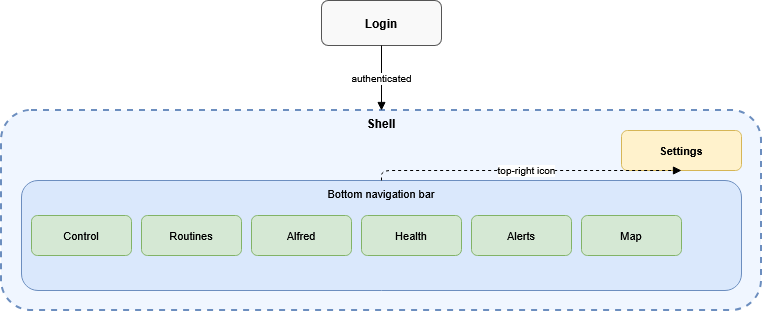
\includegraphics[width=0.85\textwidth]{images/mobile_nav.png}
\caption[Navigation structure of the Flutter mobile application]{The Flutter mobile application navigation starts from the Login screen, leading to a main bottom navigation bar with six tabs, and further to the Settings screen. Users can access Settings from any tab via the top-right icon.}
\label{fig:mobile_nav}
\end{figure}

\FloatBarrier

\subsection{Care and Schedule Page Design}
\label{subsec:reminder_calendar}

The web dashboard features a \textbf{Care \& Schedule} page with a Google Calendar-style~\cite{GoogleCalendar2024} interface supporting four colour-coded event categories: Medicine (blue), Activity (purple), Appointment (green), and Note (pink), with Month, Week, and Day view modes. The Day view features a medicine adherence progress bar and per-event Done/Edit controls, while overdue medicines are highlighted in amber. Medicine reminders (those with a fixed time and recurrence) are persisted to the backend through \texttt{/api/reminders}, enabling cross-device synchronisation. Other calendar entries (Activity, Appointment, Note) are stored in browser \texttt{localStorage} keyed by user ID. Client-side conflict detection identifies any two events that share the same HH:MM slot within a day column. It highlights the affected cards and column header in amber without requiring an additional backend query. The mobile \textbf{Routines} screen mirrors this with a horizontally scrollable 7-column weekly grid. The Month view is shown in Figure~\ref{fig:method_care_page}.


\begin{figure}[htbp]
\centering
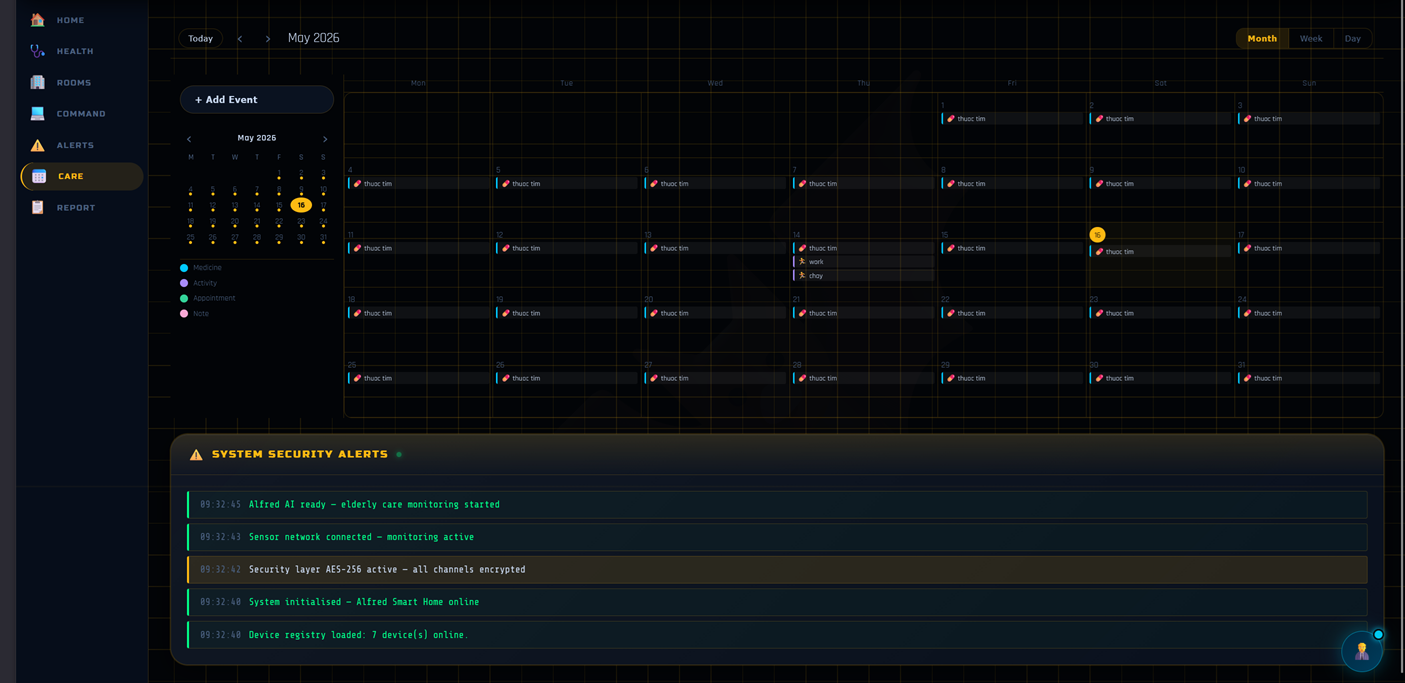
\includegraphics[width=0.90\textwidth]{images/web_care.png}
\caption[Care \& Schedule page: Month view with colour-coded event categories]{Care \& Schedule page in Month view (May 2026): monthly calendar grid displaying recurring medicine events (\textit{thuốc tim}) across all days, with activity events colour-coded by category (Medicine blue, Activity purple, Appointment green, Note pink). Left sidebar provides an Add Event button, mini calendar navigation, and legend.}
\label{fig:method_care_page}
\end{figure}

\subsection{Health Report Design}
\label{subsec:report_design}

The Report page generates two on-demand, print-optimised HTML reports.

The \textbf{Daily Report} gives a snapshot of caregiver handover, summarizing key daily metrics like medication adherence, schedule completion, and alert count, along with detailed tables of medications, events, and alerts retrieved from the backend APIs.

The \textbf{Weekly Report} gives a more general overview of the patient’s physiological state over a seven-day period, including vital-sign statistics, AI-based cardiac assessment from Alfred, alert severity distribution, and clinical notes.

Both reports open in a browser popup and are automatically sent to the print dialog via \texttt{window.print()} (Figure~\ref{fig:method_health_report}).

\begin{figure}[htbp]
\centering
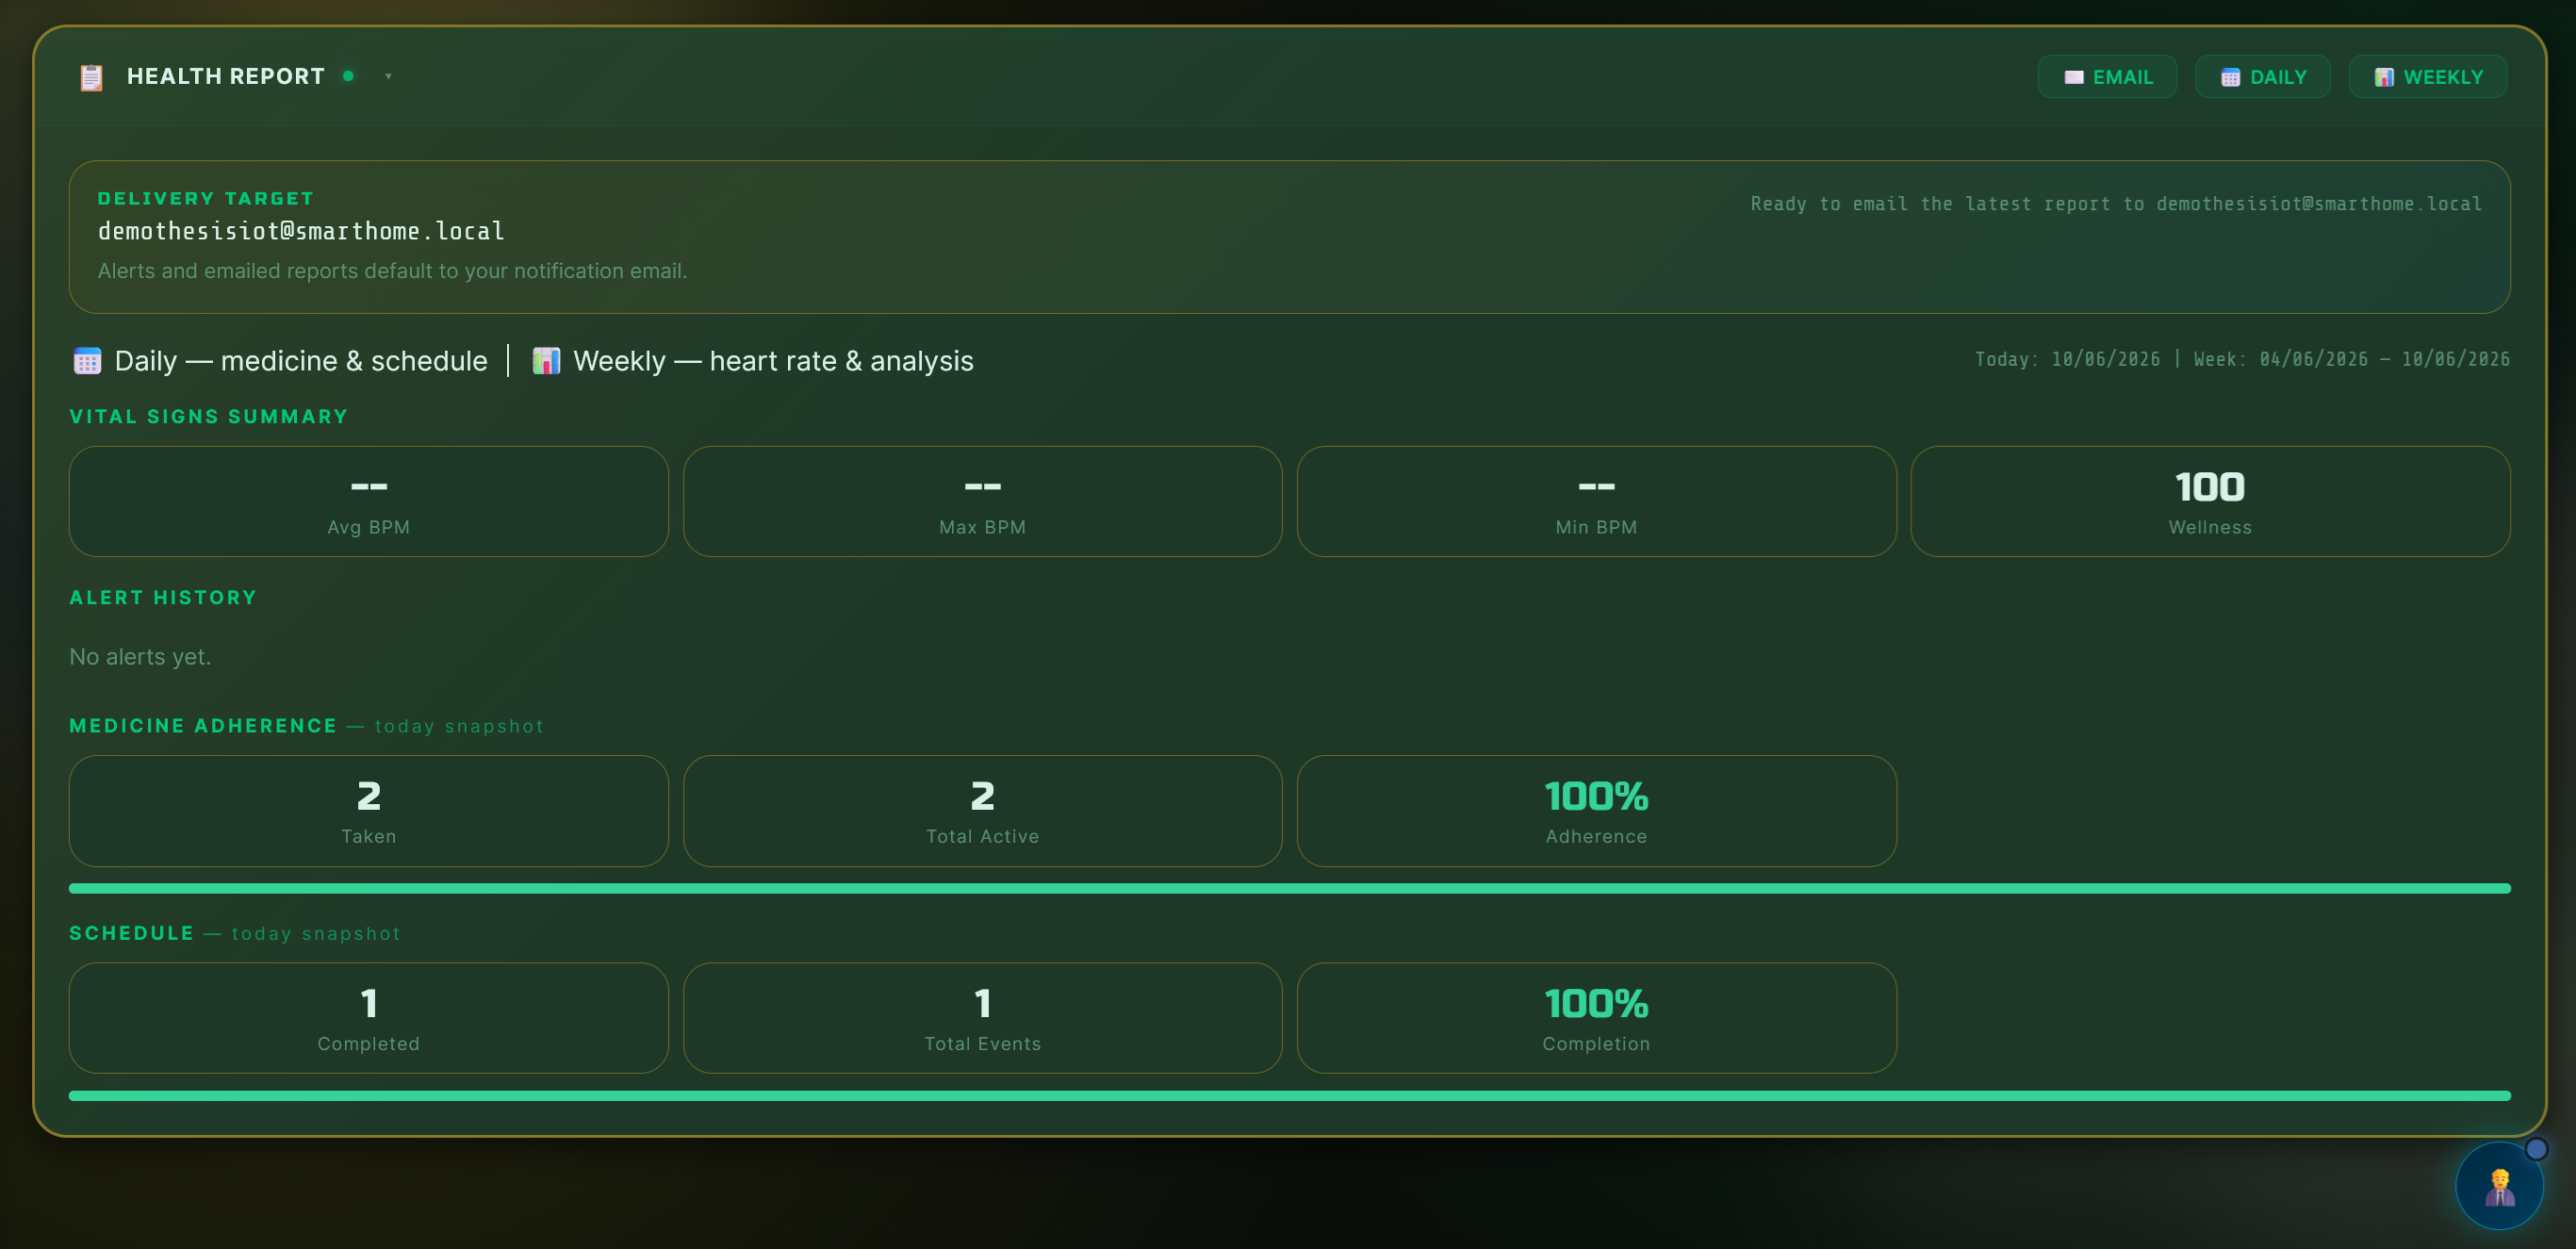
\includegraphics[width=0.82\textwidth]{images/fig_health_report_export_ui.png}
\caption[Health Report export interface]{Health Report export panel: delivery target, reporting period (weekly), vital signs summary (Avg BPM and Max BPM), alert history status, and EMAIL/PRINT export controls.}
\label{fig:method_health_report}
\end{figure}

% ─────────────────────────────────────────────────────────────
\section{Intelligent Health Analytics and AI Assistant Design}
\label{sec:ml_method}

\subsection{Heart-Rate Anomaly Detection}
\label{sec:anomaly_design}

\paragraph{Algorithm Selection Rationale}

Monitoring of the elderly requires detection of health anomalies using a method that does not rely on labelled anomaly data as real cardiac events are rare and difficult to collect ethically. The model should also support near real-time inference (under 100\,ms) and integrate naturally with a Python scikit-learn pipeline~\cite{Pedregosa2011}.

\textbf{Isolation Forest} \cite{Liu2008} was selected as it satisfies these constraints. It was preferred over the other candidate methods reviewed in Section~\ref{subsec:ml_selection} (One-Class SVM, and LSTM and dense autoencoders), which have more complex hyperparameter spaces, are slower to retrain on streaming data, and offer no clear accuracy advantage for the single-feature cardiac signal used here. The deployed Isolation Forest is benchmarked empirically against a simple fixed-threshold baseline in Section~\ref{sec:ml_validation} (Table~\ref{tab:feature_ablation}).

\paragraph{Feature Selection}

Seven candidate features are defined in the shared configuration:

\begin{enumerate}
    \item \textbf{heart\_rate} --- beats per minute from the Coospo~H6.
    \item \textbf{room\_temp} --- ambient temperature ($^\circ$C) from DHT11.
    \item \textbf{humidity} --- relative humidity (\%) from DHT11.
    \item \textbf{light\_level} --- normalised ambient light (0--100) from LDR.
    \item \textbf{hour} --- integer hour of day (0--23) for circadian context.
    \item \textbf{is\_night} --- binary: 1 if $20 \leq \text{hour}$ or $\text{hour} \leq 6$.
    \item \textbf{is\_dark} --- binary: 1 if light\_level $< 50$.
\end{enumerate}

In preliminary experiments, model performance was worse when all seven features were included. This is because each tree randomly samples from all features, making the probability of selecting \texttt{heart\_rate} only 1-in-7, which dilutes the cardiac anomaly signal. The deployed model therefore uses \textbf{heart\_rate} as its sole input. The remaining six features remain in the shared configuration and can be activated if multi-modal monitoring is added later.

The contamination parameter is selected by a grid search over nine values $\{0.010,\,0.015,\,0.020,\,0.025,\,0.030,\,0.035,\,0.040,\,0.050,\,0.060\}$, evaluating precision, recall, and anomaly F1 on a held-out synthetic set of 2\,000 samples: 1\,900 normal and 100 anomaly (50 tachycardia HR~140--210, 30 bradycardia HR~15--37, 11 moderate tachycardia HR~100--135, and 9 in-range samples where HR is normal but context is anomalous --- these last 9 are structurally undetectable by an HR-only model and set a natural recall ceiling below~1.0). Table~\ref{tab:contamination_grid} reports the full results.

\begin{table}[H]
\centering
\caption[Production contamination grid search results]{Production contamination grid search: Isolation Forest trained on UCI-healthy~+~1\,700 synthetic normals (2\,099 samples), evaluated on the 2\,000-sample synthetic labelled set. Values $\geq 0.050$ show a sharp precision drop; \texttt{contamination}~=~0.020 is selected as a conservative choice within the high-precision range.}
\label{tab:contamination_grid}
\small
\begin{tabular}{@{} c c c c l @{}}
\toprule
\textbf{Contamination} & \textbf{Precision} & \textbf{Recall} & \textbf{F1} & \textbf{Note} \\
\midrule
0.010 & 1.00 & 0.90 & 0.95 & \\
0.015 & 1.00 & 0.90 & 0.95 & \\
\textbf{0.020} & \textbf{1.00} & \textbf{0.91} & \textbf{0.95} & \textbf{Selected} \\
0.025 & 1.00 & 0.91 & 0.95 & \\
0.030 & 1.00 & 0.93 & 0.96 & \\
0.035 & 1.00 & 0.93 & 0.96 & \\
0.040 & 1.00 & 0.93 & 0.96 & \\
0.050 & 0.74 & 0.93 & 0.82 & Precision drop \\
0.060 & 0.74 & 0.94 & 0.83 & Precision drop \\
\bottomrule
\end{tabular}
\end{table}

Values 0.010--0.040 all achieve precision~1.00, meaning no false alerts on normal readings within this synthetic test set. Among these, \texttt{contamination}~=~0.020 is retained for production: it sits in the middle of the high-precision band and produces a lower alert rate than higher values, which matters more in continuous home monitoring than squeezing out an extra percentage point of recall. Values $\geq 0.050$ flag roughly one in four normal readings as anomalous --- an alert rate that would quickly cause caregiver fatigue and was ruled out on that basis.

Note that Table~\ref{tab:contamination_grid} reports F1~=~0.95 for \texttt{contamination}~=~0.020, while the UCI held-out evaluation in Table~\ref{tab:feature_ablation} (Chapter~5) reports F1~=~0.51 for the same setting. The gap comes entirely from the test set: the synthetic set here is balanced (95\% normal, 5\% anomaly) and its anomaly BPM values were generated to be clearly outside the normal band, so the model separates them easily. The UCI cohort is 84\% diseased patients whose BPMs, after the thalach approximation, overlap more with the healthy range --- a harder and more clinically realistic problem.

\paragraph{Risk Classification Design}
\label{subsec:risk_design}

Each incoming BPM reading passes through a two-layer decision pipeline before a risk level is assigned (Table~\ref{tab:risk}):

\begin{enumerate}
    \item \textbf{Layer 1 — Hard threshold (always evaluated first).}
    If BPM~$<$~50, the reading is classified as Caution (bradycardia).
    If $100 \leq \text{BPM} < 130$, it is Warning (tachycardia onset);
    if BPM~$\geq$~130, it is Critical (severe tachycardia).
    These rules fire unconditionally --- no ML score is consulted.

    \item \textbf{Layer 2 — Isolation Forest (consulted only for BPM 50--99).}
    Readings that clear Layer~1 are passed to the IF anomaly scorer.
    Within the 50--99 range, only two \emph{borderline sub-zones} activate the
    IF score: 50--59\,bpm and 96--99\,bpm.
    If the IF flags a reading in either sub-zone as an outlier, it is
    elevated to Caution.
    Readings in the clearly normal zone (60--95\,bpm) are labelled Normal
    regardless of the IF score, to suppress false positives in that range.
\end{enumerate}

This two-layer design ensures that clinically extreme values (BPM~$<$~50 or $\geq$~100) are always captured even before the IF model has been trained on sufficient patient-specific data, while the IF adds a statistical second opinion for borderline readings that fall between the hard-threshold boundaries.

\begin{table}[H]
\centering
\caption[Heart-rate risk level thresholds]{Heart-rate risk level thresholds, clinical basis, and system actions}
\label{tab:risk}
\small
\begin{tabularx}{\textwidth}{@{} l >{\RaggedRight\arraybackslash}p{2.2cm}
                                   >{\hsize=1.1\hsize\RaggedRight\arraybackslash}X
                                   >{\hsize=0.9\hsize\RaggedRight\arraybackslash}X @{}}
\toprule
\textbf{Level} & \makecell[l]{\textbf{BPM}\\\textbf{range}} & \textbf{Clinical basis} & \textbf{System action} \\
\midrule
Normal   & 50--99 &
  \begin{tblitem}
    \item AHA resting HR guideline: 60--100\,bpm~\cite{AHA2024}.
    \item Lower bound extended to 50\,bpm for physically active elderly.
  \end{tblitem} &
  \begin{tblitem}
    \item No alert.
    \item Reading persisted.
  \end{tblitem} \\
\addlinespace[4pt]
Caution  & $<50$; or IF outlier in borderline zone (50--59 or 96--99\,bpm) & Bradycardia (AHA)~\cite{AHA2024}; or borderline reading flagged as Isolation Forest outlier. IF outliers in the clearly normal zone (60--95\,bpm) are suppressed to avoid false positives. &
  \begin{tblitem}
    \item Alert logged.
    \item Socket.IO \mbox{\texttt{hr\_alert}} emitted.
  \end{tblitem} \\
\addlinespace[4pt]
Warning  & 100--129 & Tachycardia onset (AHA)~\cite{AHA2024}. &
  \begin{tblitem}
    \item Alert + Socket.IO push.
    \item Toast notification.
  \end{tblitem} \\
\addlinespace[4pt]
Critical & $\geq 130$ &
  \begin{tblitem}
    \item Severe tachycardia.
  \end{tblitem} &
  \begin{tblitem}
    \item Immediate alert, audio chime.
    \item In-app critical banner.
  \end{tblitem} \\
\bottomrule
\end{tabularx}
\end{table}

The threshold of 130 bpm for the Critical level is conservatively set below the commonly cited severe tachycardia threshold of 150 bpm to enable earlier caregiver intervention for elderly users who may tolerate rapid heart rates less well than younger adults.

\paragraph{Isolation Forest Anomaly Score}
\label{subsec:if_score}

The Isolation Forest algorithm computes an anomaly score $s(x,n)$ for each input $x$ based on the average path length $E[h(x)]$ across $T$ isolation trees, where $n$ is the subsampling size:

\begin{equation}
s(x,\,n) \;=\; 2^{-\,\dfrac{E[h(x)]}{c(n)}}
\label{eq:if_score}
\end{equation}

\noindent where $c(n)$ (Equation~\eqref{eq:cn}) represents the expected path length of an unsuccessful search in a binary search tree of $n$ nodes:

\begin{equation}
c(n) \;=\; 2\,H(n-1) - \dfrac{2(n-1)}{n},
\qquad H(i) = \ln i + 0.5772
\label{eq:cn}
\end{equation}
A score $s \to 1$ indicates a high probability of anomaly, as the average path length is short and the point is isolated quickly. A score closer to $0.5$ corresponds to a normal point with a longer average path length. In scikit-learn the
\texttt{decision\_function} returns the negative of the raw anomaly score
shifted by the contamination threshold, so negative values flag outliers.
For this system, the StandardScaler-normalised BPM is the single input
feature; the 300-tree forest then computes Equation~\eqref{eq:if_score}
and classifies the reading as INLIER or OUTLIER.

\paragraph{Anomaly Model Training Dataset}
\label{subsec:synth_data}

The production Isolation Forest is trained on \textbf{normal samples only}: all 499 UCI Heart Disease healthy records (\texttt{target\,=\,0}) plus 1\,700 synthetic normal-HR values, giving 2\,199 training samples in total (Figure~\ref{fig:ml_pipeline}).
UCI diseased records (\texttt{target\,=\,1}) are excluded from \texttt{fit()} entirely.
The synthetic samples cover sleep-time HR (50--74\,bpm) absent from the UCI dataset,
preventing over-flagging of normal nocturnal bradycardia.
Table~\ref{tab:synth_hr_ranges} shows the generation rules applied in
\texttt{\_add\_synthetic\_normals()} and \texttt{tune\_and\_retrain\_anomaly.py}.

\begin{table}[H]
\centering
\caption[Synthetic normal-HR generation rules]{Synthetic normal-HR generation rules (\texttt{\_add\_synthetic\_normals()})}
\label{tab:synth_hr_ranges}
\small
\begin{tabular}{llll}
\toprule
\textbf{Condition} & \textbf{Definition} & \textbf{HR range (bpm)} & \textbf{Rationale} \\
\midrule
Night-time & \texttt{hour}~$\geq$~20 or \texttt{hour}~$\leq$~6 & 50--74 & Resting/sleep bradycardia \\
Daytime    & otherwise                                          & 60--91 & Active resting HR         \\
\bottomrule
\end{tabular}
\end{table}

For the evaluation benchmark reported in Chapter~\ref{chap:experiments}, a separate
\textbf{80/20 split} is applied to the UCI healthy records only: 399 records (80\,\%) are used
to train a reference model with no synthetic data, and the held-out set combines the
remaining 100 healthy records with all 526 diseased records ($n=626$), providing a
clinically labelled test with no synthetic samples. Full dataset composition and
evaluation results are reported in Table~\ref{tab:train_composition} (Section~\ref{sec:ml_validation}).

\paragraph{Training Configuration}

The Isolation Forest is trained using scikit-learn~\cite{Pedregosa2011} with the following
hyperparameters, determined by grid search over nine contamination values:

\begin{itemize}
    \item \textbf{n\_estimators}: 300 trees for the production deployed model
    (higher than the default 100 to reduce variance on a small dataset);
    200 trees for the UCI evaluation benchmark, where a smaller ensemble
    is sufficient given the cleaner, purely real-data training set
    (399 UCI healthy records, no synthetic samples).
    \item \textbf{contamination}: Two values are used for different purposes.
    The UCI evaluation benchmark uses \texttt{contamination}~=~0.10, hardcoded
    in \texttt{eval\_benchmark\_model.py}. The value was arrived at by trial
    on the UCI held-out set: it shifts the Isolation Forest decision boundary
    to the point where anomaly F1 is highest, and does not correspond to any
    class proportion in the data. Because the training set contains only
    healthy records, the actual outlier rate seen during \texttt{fit()} is
    zero; 0.10 is purely a threshold knob tuned post-hoc.
    At this setting the heart-rate-only model achieves
    precision~0.96, recall~0.70, F1~0.81 on the UCI held-out test set
    (399 UCI healthy records for training, no synthetic data).
    The production-deployed model uses \texttt{contamination}~=~0.020, selected
    by the grid search in \texttt{tune\_and\_retrain\_anomaly.py} (nine values
    0.010--0.060, scored by anomaly F1 on a 2\,000-sample synthetic labelled set
    of 1\,900 normals and 100 anomalies), fitting 2\,199 normal training samples
    (1\,700 synthetic + 499 UCI healthy).
    \item \textbf{random\_state}: 42 for reproducibility.
    \item \textbf{max\_samples}: \texttt{auto} (256 per tree).
\end{itemize}

The model is trained on \textbf{normal samples only} (no labelled
anomalies are used during training) — the standard one-class setup for
Isolation Forest.

\paragraph{Model Configuration Reference}

Table~\ref{tab:model_configs} provides a single-glance map of all four Isolation
Forest configurations used across training, evaluation, and deployment.
Subsequent sections and Chapter~5 refer to these configurations by name.

\begin{table}[H]
\centering
\caption{Isolation Forest configuration map}
\label{tab:model_configs}
\small
\begin{tabularx}{\textwidth}{@{} l >{\RaggedRight\arraybackslash}X c c >{\RaggedRight\arraybackslash}X @{}}
\toprule
\textbf{Name} & \textbf{Training data} & \textbf{Contam.} & \textbf{Trees} & \textbf{Purpose} \\
\midrule
Production deployed
  & 1\,700 synthetic + 499 UCI healthy = 2\,199
  & 0.020 & 300
  & Runs live in the backend; calibrated for low false-alarm rate \\
\addlinespace[3pt]
Production evaluated
  & 1\,700 synthetic + 399 UCI healthy = 2\,099
  & 0.020 & 300
  & Same as deployed but trained on 399 (not 499) healthy to keep 100 healthy test records unseen; used in Table~\ref{tab:feature_ablation} \\
\addlinespace[3pt]
Benchmark
  & 399 UCI healthy only
  & 0.10 & 200
  & Clean UCI 80/20 evaluation; source of P\,0.96 / R\,0.70 / F1\,0.81 headline metrics \\
\addlinespace[3pt]
Grid-search tuning
  & 2\,000 synthetic labelled (1\,900 normal + 100 anomaly)
  & 0.010--0.060 & 300
  & Contamination selection only; not used for final evaluation \\
\bottomrule
\end{tabularx}
\end{table}

Figure~\ref{fig:ml_pipeline} summarises the two-phase pipeline: the
offline training phase (initial run at server startup, then repeated
weekly via APScheduler) and the online inference path
(executed per incoming BPM reading).

\begin{figure}[H]
\centering
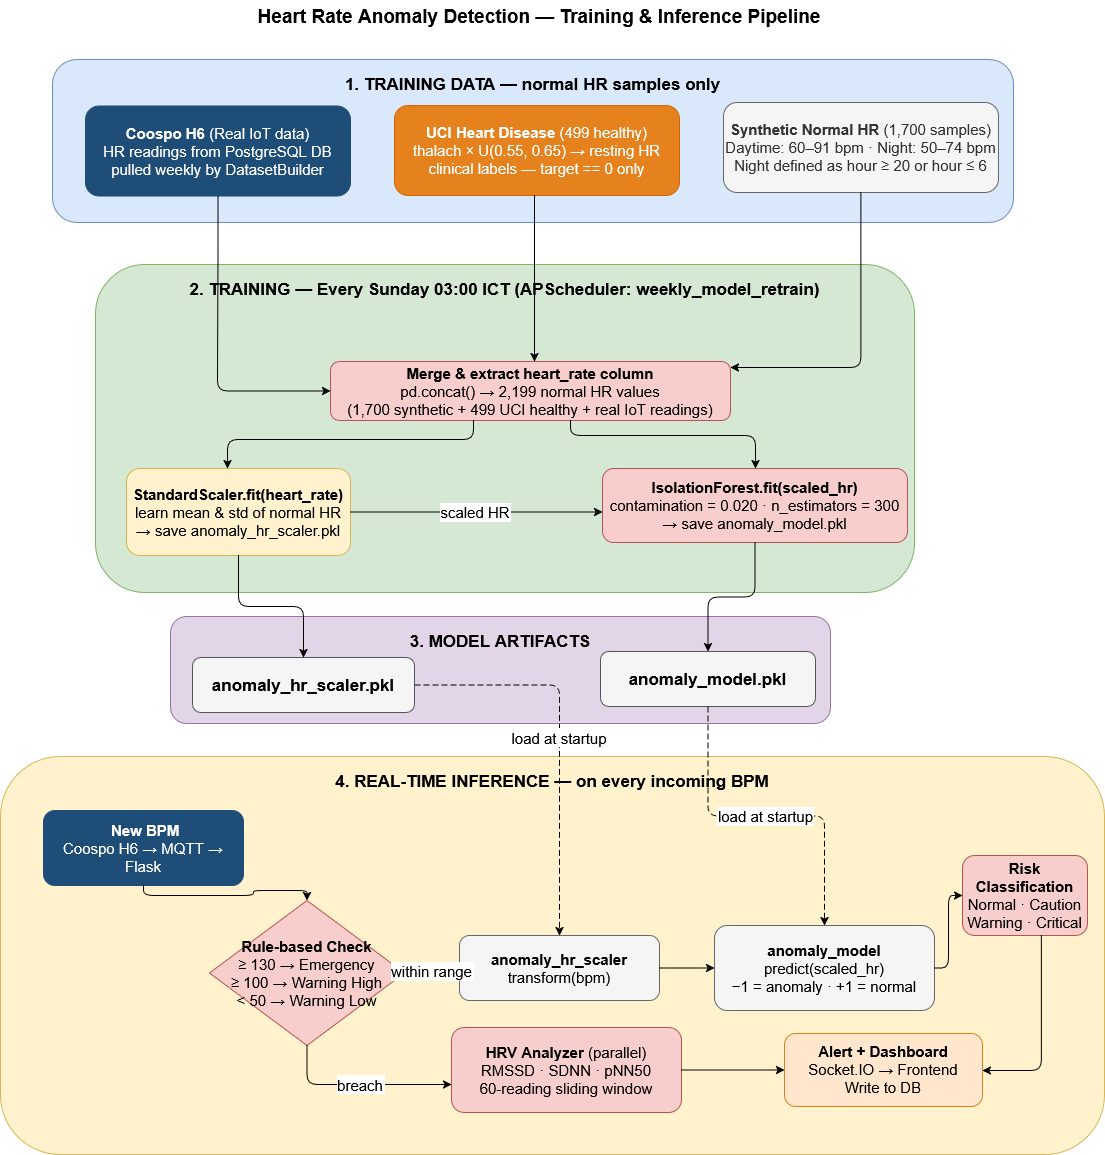
\includegraphics[width=\textwidth]{images/fig_hr_anomaly_pipeline.png}
\caption[Heart rate anomaly detection pipeline: training and inference]{%
         Heart rate anomaly detection pipeline.
         \textbf{Training} (top, repeated every Sunday at 03:00 by
         \texttt{weekly\_model\_retrain}): normal HR samples from three
         sources — real IoT readings (Coospo H6), 499 UCI Heart Disease
         healthy records converted from \textit{thalach}, and 1\,700
         synthetic day/night samples — are merged, scaled with a
         dedicated \texttt{StandardScaler}, and used to fit an
         \texttt{IsolationForest} (\texttt{contamination}=0.020,
         \texttt{n\_estimators}=300).
         \textbf{Inference} (bottom, per incoming BPM): each reading
         passes a rule-based threshold check first; readings within range
         are forwarded to the scaler then the model for anomaly scoring
         and risk classification.}
\label{fig:ml_pipeline}
\end{figure}

\FloatBarrier

\paragraph{Periodic Model Retraining}
\label{subsec:periodic_retrain}

Two separate training scripts serve distinct roles in this system.
\texttt{tune\_and\_retrain\_anomaly.py} is a standalone offline script
that produced the initial model and all evaluation metrics reported in
Chapter~\ref{chap:experiments} (Table~\ref{tab:feature_ablation}); it
operates without database access and trains exclusively on the
UCI~+~synthetic baseline (2\,199 samples).
\texttt{train\_pipeline.py}, by contrast, is the live backend pipeline
invoked by the scheduler: it pulls accumulated sensor readings directly
from the database, merges them with the UCI baseline and a shrinking
synthetic buffer, and overwrites the deployed model artefacts in place.
The two scripts share the same contamination value (0.020) and model
architecture but differ in data composition as real IoT readings build up
over time.

The Isolation Forest and the three companion models (automation classifier,
mood classifier, shared scaler) are retrained automatically every Sunday
at 03:00~(Asia/Ho\_Chi\_Minh) by an APScheduler \texttt{BackgroundScheduler}
job registered at server startup (\texttt{weekly\_model\_retrain}).
The job calls \texttt{run\_full\_training()} inside a Flask application
context so that \texttt{DatasetBuilder} can access the database.

Each retrain pass merges three data sources into a shared DataFrame:
\begin{enumerate}
    \item \textbf{Real IoT sensor data} (from the \texttt{sensor\_data} table) ---
    accumulated readings from the deployed ESP32 node and Coospo~H6 device,
    resampled at 5-minute intervals.
    \item \textbf{UCI Heart Disease healthy records} (499 rows, \texttt{target}~=~0)
    --- a fixed clinical baseline loaded from \texttt{data/heart\_disease.csv}.
    \item \textbf{Synthetic normal samples} --- the count decreases automatically
    as real IoT data grows, following the five-stage dilution schedule in
    Table~\ref{tab:dilution}.
\end{enumerate}

The four models trained from this DataFrame use different feature subsets.
The \textbf{anomaly model} extracts only the \texttt{heart\_rate} column and
fits a dedicated HR scaler (\texttt{anomaly\_hr\_scaler.pkl}), keeping
\texttt{contamination}~=~0.020 as established by grid search.
Room context features (temperature, humidity, light) are excluded because
they dilute the cardiac signal: each Isolation Forest tree samples uniformly
from all features, so adding six context columns reduces the probability of
selecting \texttt{heart\_rate} to 1-in-7~\cite{Liu2008}.
The \textbf{automation} and \textbf{physiological state (mood)} classifiers
use the full 7-feature scaled matrix; their design and label sources are
described in Section~\ref{sec:companion_classifiers}.

\begin{table}[H]
\centering
\caption[Synthetic dilution schedule]{Synthetic dilution schedule in \texttt{\_choose\_synthetic\_samples()}}
\label{tab:dilution}
\small
\begin{tabular}{@{} l r l @{}}
\toprule
\textbf{Stage} & \textbf{Synthetic samples added} & \textbf{Rationale} \\
\midrule
$<$10 real rows       & 1\,700 & Cold-start bootstrap \\
10--599 real rows     & 1\,700 & UCI-seed phase (matching baseline) \\
600--999 real rows    & $\max(300,\ \lfloor\text{real}{\times}0.50\rfloor)$ & Growth phase \\
1\,000--4\,999 real rows & $\max(40,\ \lfloor\text{real}{\times}0.20\rfloor)$ & Mature phase \\
$\geq$5\,000 real rows   & 0 & Real-dominant, no synthetic needed \\
\bottomrule
\end{tabular}
\end{table}

As deployment time increases, the model progressively shifts from
synthetic-dominant to real-data-dominant training, improving its fit
to the specific user's circadian HR patterns.
Job failures are caught and logged at \texttt{ERROR} level; they do not
propagate to the scheduler thread, so a failed retrain does not affect
the running inference pipeline.

% ─────────────────────────────────────────────────────────────
\subsection{Companion Classifiers: Physiological State and Automation}
\label{sec:companion_classifiers}

The training pipeline produces two RandomForest classifiers alongside the
anomaly model.  They share the same 7-feature scaled matrix and are retrained
weekly, but serve entirely different purposes from the anomaly detector.

\paragraph{Physiological State (Mood) Classifier}

The physiological state classifier assigns each incoming BPM reading one of
seven context-aware labels: \texttt{EMERGENCY}, \texttt{ELEVATED},
\texttt{QUIET}, \texttt{SLEEP}, \texttt{REST}, \texttt{ACTIVE}, or
\texttt{NORMAL}.  Because no labelled dataset of real physiological states
with time-stamped sensor readings exists, the training labels are generated
by a deterministic rule function (\texttt{\_calc\_mood}) that maps sensor
values to states using published elderly HR norms and circadian patterns:

\begin{itemize}
    \item \textbf{EMERGENCY}: HR~$\geq130$\,bpm (checked first — unconditional)
    \item \textbf{ELEVATED}: HR~$\geq100$\,bpm
    \item \textbf{QUIET}: night-time ($\text{is\_night}=1$) and light\_level~$<20$ (0--100 scale)
    \item \textbf{SLEEP}: night-time and HR~$<65$\,bpm
    \item \textbf{REST}: HR~$<60$\,bpm with elevated room temperature ($>28\,^\circ$C)
    \item \textbf{ACTIVE}: HR~$\geq80$\,bpm with high ambient light (light\_level~$>60$, 0--100 scale)
    \item \textbf{NORMAL}: all other readings — none of the above conditions met (fallback label)
\end{itemize}

Rather than applying the rules as a direct lookup, a RandomForest is trained on pseudo-labels produced by \texttt{\_calc\_mood} to handle readings that fall between hard thresholds --- the model inherits the label semantics of the rules but uses the surrounding training distribution to assign a class rather than forcing a binary condition check. It cannot discover categories beyond what the rules define, and its boundary behaviour has not been validated against ground-truth physiological annotations (see evaluation note below).
The predicted state is attached to each \texttt{hr\_alert} Socket.IO event, stored in \texttt{patient\_hr\_record}, and exported in health report PDFs in the ``RISK\,/\,MOOD'' column.

The automation classifier is trained using real user behaviour: labels (\texttt{action\_label}) derived from the \texttt{ControlLog} table, matched with sensor readings in the 2-minute window prior to the device action. 
The model can improve as the household accumulates usage data through weekly retraining. \textbf{Evaluation note.} Neither classifier has been independently and quantitatively evaluated. The mood classifier labels are purely determined by \texttt{\_calc\_mood}. Boundary smoothing by RandomForest cannot be validated without ground-truth annotations. The automation classifier does not have enough logged events at the prototype stage to measure meaningful precision/recall. A quantitative evaluation of both is left for future work (Section~\ref{sec:future}).

% ─────────────────────────────────────────────────────────────
\subsection{Alfred AI Assistant}
\label{sec:alfred_method}

Alfred is a conversational assistant for health monitoring and smart home control. It runs in one of three inference modes, selectable per request:
\begin{itemize}
\item \textbf{llm} (default): The full 3-layer pipeline. The message goes through the deterministic Rule layer (device control, mood detection, keyword matching) first. If no match is found, it falls back to an Ollama \texttt{qwen2.5:3b} intent parser. If no intent is found, it is passed to a context-enriched Ollama chat call.

\item \textbf{rule}: Uses only deterministic keyword and pattern matching. It runs entirely offline with minimal latency and provides a clarification fallback when no rule matches.

\item \textbf{gemini}: Sends the context-enriched prompt to Google Gemini~2.5~Flash via the \texttt{google-genai} SDK. If the cloud service is unavailable, a Rule engine fallback response is returned rather than switching inference paths.

\end{itemize}

A frontend \textbf{Compare} overlay calls \texttt{rule}, \texttt{llm}, and
\texttt{gemini} modes sequentially and presents the three responses
side-by-side. Before each inference call, the backend injects live device
states and sensor readings into the prompt, ensuring Alfred always has access
to current home state without a retrieval-augmented architecture.

\paragraph{Context injection versus retrieval-augmented generation.}
\label{par:context_vs_rag}
A conventional RAG pipeline retrieves document chunks from a vector store before generating a response. That design is well-suited to large, slowly changing knowledge bases --- medical literature, product manuals, FAQ corpora --- where the information is too voluminous to fit in a prompt and is updated infrequently enough that a slightly stale retrieval result is acceptable. Alfred operates over a fundamentally different kind of data. The house context --- room names, relay states, sensor readings --- is small enough to serialize into a short prompt prefix, is authoritative at request time because it is read directly from the live database, and changes fast enough that a cached embedding in a vector store would be stale within seconds of a relay toggle. Under these conditions, direct injection is not a simplification of RAG; it is the appropriate design choice. A retrieval step would add embedding-query latency and introduce the risk of serving outdated state without providing any benefit that is not already met by a direct database read.

The practical limit of this approach is context window size. At the current prototype scale --- one ESP32 node, up to eight sensors, and two to five devices per room --- the serialized house prefix fits comfortably within 100 tokens, well inside the limits of both \texttt{qwen2.5:3b} and Gemini~2.5~Flash. If the deployment were extended to dozens of rooms and hundreds of devices, selective injection (e.g., filtering to the user's active room before prompt construction) would be necessary. That path is noted as a Phase~2 architectural consideration in Section~\ref{sec:future}.

\paragraph{Local LLM Selection Rationale}
\label{subsec:llm_selection}

\texttt{qwen2.5:3b} (Q4\_K\_M, $\approx$2\,GB) was selected for local inference for three reasons: (1) it runs comfortably on the 16\,GB development machine alongside the Flask backend and MySQL process; (2) it supports Vietnamese and English without translation, enabling mixed-language input; and (3) preliminary tests showed that it follows the desired JSON schema (\texttt{\{action, target\_device, value, reply\}}) more reliably than the alternatives tested (\texttt{gemma2:2b}, \texttt{phi3.5-mini}). A formal, multi-model comparison is deferred to future work (Section~\ref{sec:future}).

\paragraph{Mode-wise Request Processing}

The REST endpoint is the same for all chat modes: \path{POST /api/ai/chat}, with the same fields: \path{message}, \path{mode} and \path{language}. The difference is that \path{AIUseCase.handle\_chat()} interprets the message against the real-time house context that was loaded. Table~\ref{tab:alfred_mode_behavior} illustrates the different handling of the same utterance across the three modes.

\begin{table}[H]
\centering
\caption[Alfred utterance handling across modes]{How the same utterance is handled across Alfred modes}
\label{tab:alfred_mode_behavior}
\small
\begin{tabularx}{\textwidth}{@{} l >{\hsize=0.55\hsize\RaggedRight\arraybackslash}X >{\hsize=1.45\hsize\RaggedRight\arraybackslash}X @{}}
\toprule
\textbf{Mode} & \textbf{Backend path} & \textbf{Example behavior for ``nóng quá''} \\
\midrule
LLM        & Rule $\to$ Intent Parser $\to$ Ollama chat
           & Environmental keyword ``nóng'' matched by Rule layer; fan and AC scenario suggested with a confirmation prompt. If Rule did not match, Intent Parser would parse intent; Chat LLM handles open-ended fallback. \\
\addlinespace[4pt]
Rule       & Rule engine only (keyword/pattern)
           & ``nóng'' matches the \textit{hot} environmental intent; returns a device suggestion with confirmation prompt. If unmatched, returns clarification fallback --- no LLM call made. \\
\addlinespace[4pt]
Gemini     & Rule $\to$ Gemini 2.5 Flash (cloud)
           & Rule layer runs first --- ``nóng'' is caught and a confirmation prompt returned, same as Rule mode. If Rule misses, the context-enriched prompt goes to Gemini Flash. API unavailability falls back to the Rule clarification reply. \\
\bottomrule
\end{tabularx}
\end{table}

In short, there is no separate frontend endpoint per mode, mode selection changes backend reasoning strategy, not the transport path. Table~\ref{tab:alfred_layer_matrix} summarises which layers are activated in each mode.

\begin{table}[H]
\centering
\caption{Layer activation per Alfred inference mode}
\label{tab:alfred_layer_matrix}
\small
\begin{tabularx}{\textwidth}{@{}l X X X@{}}
\toprule
\textbf{Mode} & \makecell[l]{\textbf{Layer 1 —}\\\textbf{Rule Engine}} & \makecell[l]{\textbf{Layer 2 —}\\\textbf{Intent Parser}} & \makecell[l]{\textbf{Layer 3 —}\\\textbf{Chat LLM}} \\
\midrule
\texttt{llm}    & \checkmark\ keyword/pattern match & \checkmark\ Ollama (if Rule misses)  & \checkmark\ Ollama (if Intent misses) \\
\texttt{rule}   & \checkmark\ keyword/pattern match & \texttimes\ stops here               & \texttimes\ not called \\
\texttt{gemini} & \checkmark\ keyword/pattern match & \texttimes\ bypassed$^\dagger$        & \checkmark\ Gemini Flash \\
\bottomrule
\end{tabularx}
\smallskip\noindent{\footnotesize$^\dagger$ Gemini Flash handles intent classification and response generation in a single cloud call, so there is no need for a separate intent-parser step.}
\end{table}

\paragraph{Layer design rationale.}
The three-layer LLM pipeline assigns each layer a distinct role matched to its cost and latency profile:

\begin{itemize}
    \item \textbf{Layer~1 (Rule)} handles the majority of everyday commands --- device on/off, mood detection, room queries --- with deterministic keyword matching at negligible latency and zero API cost. It is always executed first in LLM and Gemini modes because it covers the most common intents cheaply.

    \item \textbf{Layer~2 (Intent Parser)} is a lightweight Ollama call ($\approx$100-token prompt) whose sole job is to classify an unmatched message into a fixed schema \texttt{\{intent, action, device\_type, room\}}. Rule is not reused here because if a message did not match Layer~1 it will not match again; Gemini is not used because a structured classification task does not justify cloud API latency or cost.

    \item \textbf{Layer~3 (Chat LLM)} generates the final natural-language response with full house-context injection. Gemini mode skips Layer~2 entirely and calls Gemini once for both intent and response, since Gemini can handle both classification and generation in one call.
\end{itemize}


Every incoming message runs through a nine-step early-exit waterfall in \texttt{AIUseCase.handle\_chat()}. The steps are checked in order, and the first one to match wins: as soon as a step handles the message and returns, nothing below it executes.

\textbf{Step~1} (SOS) outranks everything else. A distress keyword fires a critical alert, emails the caregiver, and returns before any other logic gets a look in. \textbf{Step~2} (FAQ) answers predictable platform questions from a hardcoded table, and only in rule mode, so the system never spends an LLM call on them. \textbf{Step~3} (Pending) clears a queued yes/no confirmation, either running the stored MQTT command or dropping it. \textbf{Step~4} (Schedule) reacts to a time or recurrence cue, parsing the cron expression through \texttt{\_apply\_daypart()} and asking for a specific clock time when the hour is ambiguous.

\textbf{Step~5} (Info query) pulls sensor, health, or device-status answers straight from the live house-context object and sends no MQTT command at all. \textbf{Step~6} (Device control) identifies target devices with word-boundary regular expressions, resolves the room, and stores a pending confirmation before it publishes anything. That two-step guard is deliberate: a stray keyword match should never flip a relay on its own. \textbf{Steps~7--8} (Small-talk and Mood) field greetings and read mood keywords to suggest a lighting or climate change, again pausing for confirmation whenever a real device would be touched.

\textbf{Step~9} (Fallback) is the only step whose behaviour depends on the mode. In \texttt{rule} mode it just returns a clarification prompt and calls no model. In \texttt{gemini} mode it forwards a context-enriched prompt to Gemini~2.5~Flash. In \texttt{llm} mode it calls \texttt{parse\_intent()} for a structured \texttt{\{intent, action, device\_type, room\}} classification, then branches on the result: \textit{control} resolves devices and stores a confirmation, \textit{query} answers from live context, \textit{chat} returns the model's reply, and \textit{add}/\textit{delete} run device-registry CRUD.

\paragraph{Alfred End-to-End Processing Flow}
\label{subsec:alfred_e2e_flow}

\texttt{AIUseCase.handle\_chat()} first loads a live house-context object (rooms, device relay states, latest sensor readings), cached per user with a 10-second TTL. When passed to an LLM, this context is serialized into a compact prompt prefix (e.g., \texttt{"Living Room: den\_1 (ON), quat\_1 (OFF)"}) to ground the model in the current home state without overflowing the context window. What happens next depends on the selected mode:

\begin{itemize}
   \item \textbf{LLM mode} runs the complete three-layer pipeline via the local Ollama backend. The message hits the deterministic Rule layer first (keyword matching, device control, mood and scenario detection). If nothing matches, a lightweight Ollama intent-parser call (\textasciitilde{}100-token prompt) classifies the intent as \texttt{control}, \texttt{query}, or \texttt{chat}. Anything still unresolved falls through to a context-enriched Ollama chat call where the full house structure and device codes are injected into the prompt.

\item \textbf{Rule mode} executes only the Rule layer and returns a clarification fallback if nothing matches --- no LLM call is made.

\item \textbf{Gemini mode} first executes the Rule layer and if unmatched, forwards the context-enriched prompt to Google Gemini~2.5~Flash. If the Gemini API is unavailable, the mode returns the Rule engine's clarification fallback rather than switching to the Ollama path.

\end{itemize}

\paragraph{Real-time device resolution.} \texttt{alfred\_knowledge.py} only stores device categories (e.g., \texttt{"ac"}, \texttt{"fan"}), not specific identifiers. If a rule matches, \texttt{AIUseCase} resolves the category to physical devices with \texttt{\_find\_devices\_by\_category()}, filtered by the room the user is currently in (set by double-clicking a room on the floor plan). If there is no such device, the action is skipped. If there are devices in more than one room, the backend asks the user to select.

\paragraph{Two-step confirmation.}
Alfred \emph{does not} execute immediately when it recognizes a device action. Instead, it stores a \texttt{pending\_action} and responds with a confirmation prompt. If the answer is affirmative (\textit{có}, \textit{yes}, \textit{đồng ý}), it calls \texttt{DeviceUseCase.set\_device()}, which publishes the MQTT command (TLS port~8883) and broadcasts the new state via Socket.IO. The pending action times out after 90 seconds. Only scheduled automation rules can run automatically without confirmation.

\paragraph{Multi-room disambiguation}
A related case arises when a matched scenario involves devices spread across several rooms. Alfred cannot safely assume which room to act on, so it asks the user to specify. The narrowed plan is held in \texttt{pending\_action} and a second confirmation is required before anything runs. One shortcut exists: if the user has already indicated their current location by double-clicking a room on the floor plan, the system filters the plan down to that room and skips straight to the confirmation step. Even so, the command is never sent without a reply from the user.

\paragraph{Rule Engine Keyword and Intent Taxonomy} \label{sec:alfred_rule_keywords}

Keyword matching in \texttt{alfred\_knowledge.py} is organised into three groups, evaluated by the Rule engine using case-insensitive substring search:

\begin{itemize}
    \item \textbf{Mood Profiles} (\texttt{MOOD\_PROFILES}) --- eight emotional states, ranging from happy and excited to sick and stressed, each paired with lighting adjustments, climate presets, and optional music or film suggestions.

    \item \textbf{Environmental Intents} (\texttt{ENVIRONMENTAL\_INTENTS}) --- four physical-condition triggers (\textit{hot}, \textit{cold}, \textit{dark}, \textit{bright}) that map directly to device actions. Rather than referencing specific device names, each entry targets a \texttt{category} value (e.g. \texttt{"fan"}, \texttt{"ac"}, \texttt{"light"}) that the system resolves to the actual installed device at query time. This means adding a new fan or replacing a light requires no change to the intent definitions. As a concrete example, saying ``too hot'' activates the \textit{hot} intent: the fan turns on at speed~3 and the air conditioner is set to 24\,°C.

    \item \textbf{Device Scenarios} (\texttt{ALFRED\_SCENARIOS}) --- eleven activity-based presets covering common routines such as going to sleep, studying, watching a film, or leaving the house. The four environmental entries in this dictionary point back to \texttt{ENVIRONMENTAL\_INTENTS} rather than repeating the definitions, so adjusting a default --- the fan speed when it feels too hot, for example --- only ever needs changing in one place.
\end{itemize}

The taxonomy covers around 20 intent categories and roughly 200 Vietnamese--English keyword triggers in total (see Appendix~\ref{app:alfred_keywords}, Table~\ref{tab:alfred_rule_keywords}). Scenarios and environmental intents are checked first; mood profiles follow. If nothing matches, the message moves on to the LLM step.

\paragraph{Natural Language Device Scheduling}

Before the LLM step, Alfred also checks whether the user is trying to set up a recurring device schedule. A dedicated \texttt{schedule\_intent\_parser} scans the message for a device reference, a clock time, and a recurrence pattern using a set of Vietnamese--English regex rules. Recognised patterns include \textit{daily}, \textit{weekday}, \textit{weekend}, and \textit{specific days of week}: for example, ``turn off the fan on Monday and Thursday at 9 pm'' is parsed into the cron expression \texttt{0 21 * * 1,4} and written to the \texttt{schedules} table. Day names in both languages are matched with word-boundary guards so that ``thu'' in ``thursday'' does not accidentally match the Vietnamese abbreviation ``T5.'' If only some components are present (e.g.\ a day name but no device), Alfred asks a follow-up question rather than guessing. Confirmed schedules are visible on the Care~\&~Schedule page and can be edited or deleted from there.

% ─────────────────────────────────────────────────────────────
\section{System Interaction Design}
\label{sec:seq_method}

Two sequence diagrams illustrate the critical runtime data flows.
Figure~\ref{fig:seq_device_method} shows the end-to-end path of a
user-initiated device toggle command from the web dashboard through the
Flask REST API and EMQX broker to the ESP32 relay, and back as a Socket.IO
confirmation event. Figure~\ref{fig:seq_health_method} shows the anomaly
detection path from a BLE heart-rate reading through to a real-time
client alert.

\begin{landscape}
\begin{figure}[p]
\centering
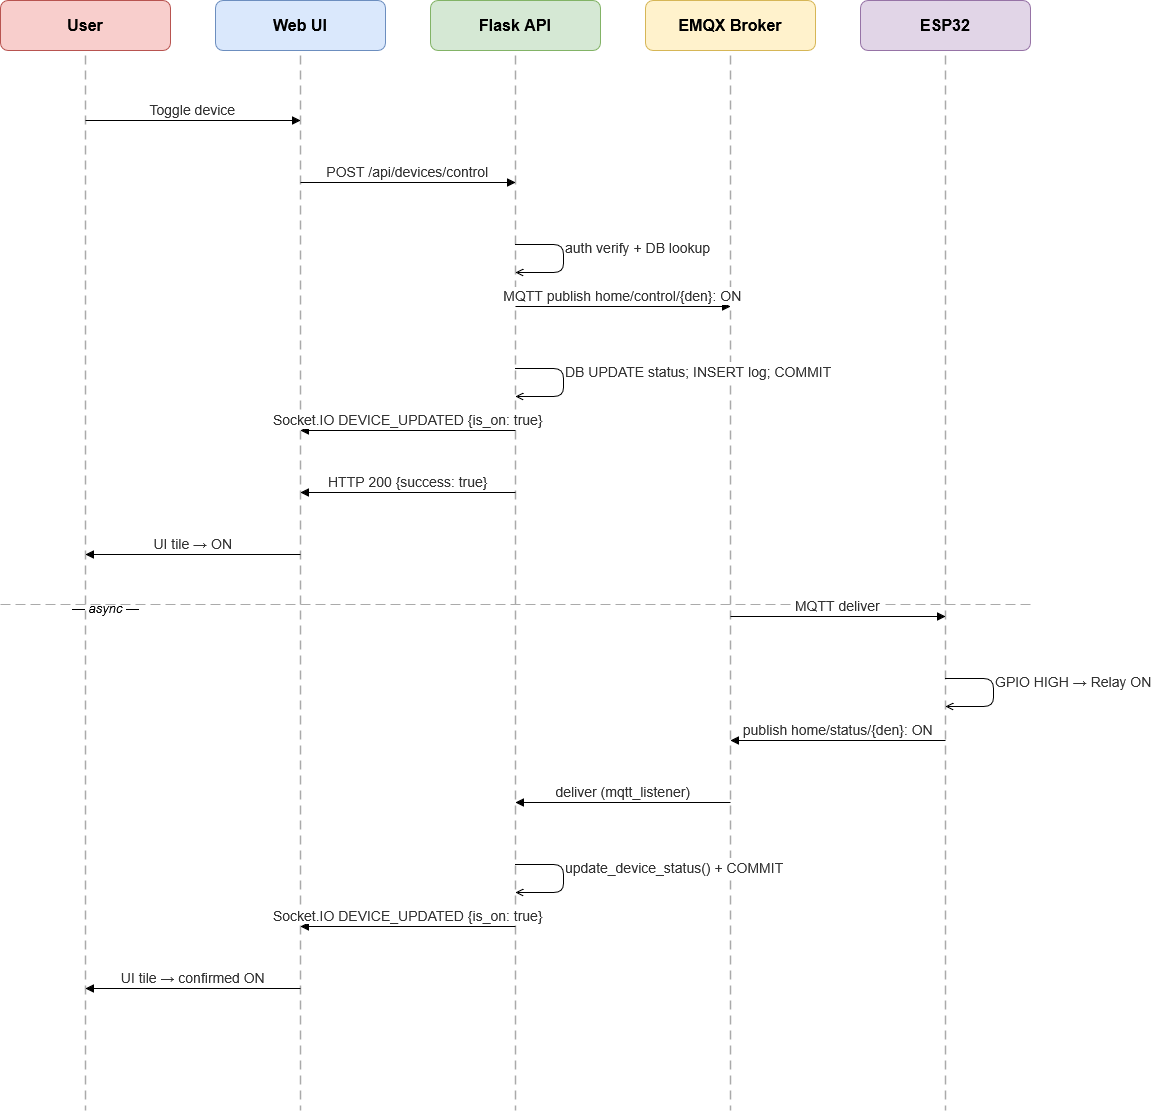
\includegraphics[width=\linewidth,height=0.80\textwidth,keepaspectratio]{images/fig_seq_s1.png}
\caption[Sequence S1: device control flow]{Sequence S1: end-to-end device control flow from web dashboard to ESP32 relay and back via Socket.IO.}
\label{fig:seq_device_method}
\end{figure}
\end{landscape}

\begin{landscape}
\begin{figure}[p]
\centering
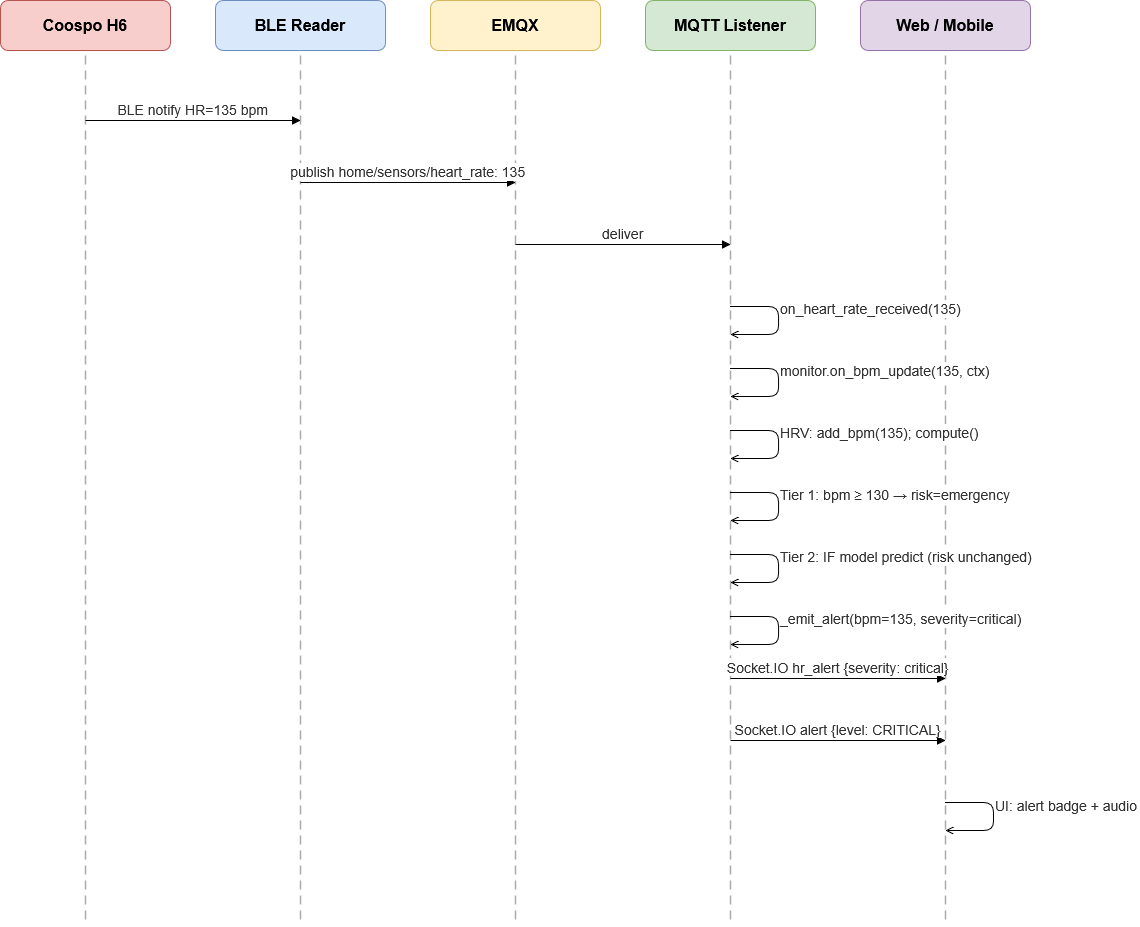
\includegraphics[width=\linewidth,height=0.80\textwidth,keepaspectratio]{images/fig_seq_s2.png}
\caption[Sequence S2: BLE heart-rate alert flow]{Sequence S2: BLE heart-rate reading to critical alert propagation across all system layers.}
\label{fig:seq_health_method}
\end{figure}
\end{landscape}



\chapter{IMPLEMENTATION AND RESULTS}
\label{chap:experiments}

This chapter documents the implementation experiments and validation results across the hardware node, backend services, web interface, and mobile app. The anomaly detection model evaluation is in Chapter~5.

\section{Experimental Setup and Validation Protocol}
\label{sec:exp_setup}

The validation campaign described in this chapter has a structure that can be repeated for all system layers (hardware node, backend services, web interface and mobile app). For each experiment the procedure is documented with (1) the input trigger, (2) the expected observable outcome, (3) the artefact collected (terminal output, API response, screenshot or runtime event) and (4) the pass/fail decision.

This thesis is based on the functional validation of an end-to-end prototype, therefore, the results of the deterministic scenario are emphasized in Chapter~\ref{chap:experiments}. Chapter~5 (Section~\ref{subsec:latency_protocol}) reports a preliminary latency benchmark (10 trials, relay ON command), and Chapter~6 identifies long-duration reliability benchmarking as a formal follow-up experiment.

% ─────────────────────────────────────────────────────────────

\section{Implementation}
\label{sec:implementation}

\subsection{Firmware}
\label{sec:hw_impl}

The ESP32 firmware is based on the Arduino core for ESP32 (version~2.x) and uses five libraries: \texttt{WiFiClientSecure.h} (TLS), \texttt{PubSubClient} (MQTT), \texttt{DHT} (Adafruit) for the DHT11, \texttt{Wire.h} (I2C), and \texttt{LiquidCrystal\_I2C} for an optional 16x2 LCD.

On startup, it connects to Wi-Fi, loads credentials from a header file, and registers \texttt{mqttCallback}. The main \texttt{loop()} runs without a fixed delay to keep MQTT alive, publish sensor readings every 5 seconds (retained, QoS~0), and handle relay buttons with 200\,ms debounce. All tasks run sequentially on the same core.

During initialisation, it scans for I2C backpack addresses (0x27 and 0x3F) and enables the LCD only if found, allowing normal operation without the display.

% ─────────────────────────────────────────────────────────────
\subsection{REST API Endpoints}
\label{sec:backend_impl}

The backend exposes around 80 REST endpoints, grouped into ten functional groups, all prefixed by \path{/api/}. Table~\ref{tab:api} gives an overview of each group; The complete specification can be found in the built-in Swagger UI at \path{/api/docs}.

\begin{table}[H]
\centering
\caption{REST API endpoint groups}
\label{tab:api}
\small
\begin{tabularx}{\textwidth}{@{} >{\raggedright\arraybackslash}p{2.8cm} c >{\RaggedRight\arraybackslash}X @{}}
\toprule
\textbf{Group} & \textbf{Routes} & \textbf{Responsibility} \\
\midrule
Authentication   & 9  & Login, register, signed HttpOnly cookie issuance, profile update, forgot/reset password, account deletion \\
Devices          & 11 & List devices, send ON/OFF via MQTT, poll status snapshot, history, position update, schema \\
Rooms \& Map     & 10 & CRUD room polygons, list/save floor layout JSON for the map editor \\
Patient \& Health & 8  & Patient profile, heart-rate records, PDF report export \\
Care / Medicine  & 8  & CRUD medicine reminders, mark reminder as taken; CRUD care-calendar events (activities, appointments, notes) \\
Alerts           & 14 & Paginated alert list, acknowledge, delete, bulk-delete, SOS, mute/suggestion preferences \\
Automation       & 8  & CRUD automation rules and scheduled device actions \\
AI Chat          & 3  & Alfred chat inference (rule/LLM/Gemini modes), sensor analysis, status check \\
BLE              & 5  & Coospo H6 BLE reader: connect, disconnect, status, HR alert stream, debug alert (disabled by default) \\
Admin            & 3  & List users, delete account, promote/demote role (admin only) \\
\bottomrule
\end{tabularx}
\end{table}

\subsection{Real-Time Communication}

The application factory initializes a Socket.IO server using Flask-SocketIO.
The backend emits ten named events to connected clients:
\texttt{device\_status} (relay state confirmed by ESP32), \texttt{device\_list\_changed} (device added, removed or updated), \texttt{alert} (anomaly or medicine alert logged), \texttt{hr\_alert} (heart-rate threshold crossed or outlier from Isolation Forest), \texttt{hrv\_update} (latest heart-rate reading broadcast every 15\,s while BPM data is flowing), \texttt{ai\_mood} (Alfred mood/scenario suggestion), \texttt{ai\_advice} (Alfred inline advice), \texttt{ai\_explain} (Alfred environmental action suggestion), \texttt{schedule\_reminder} (cron-based device schedule popup when \texttt{remind\_only} is set), \texttt{map\_layout\_updated} (floor-plan zone configuration changed).
Web and mobile clients join a user-specific Socket.IO room after authentication, providing data isolation between users.

\subsection{Security Implementation}

Protected API endpoints require a signed HttpOnly session cookie (\texttt{batman\_os\_auth} --- named after Alfred's employer in the project theme) generated with \path{itsdangerous}. The cookie token is signed with Flask's \path{SECRET\_KEY} and validated with a maximum lifetime of seven days using \path{URLSafeTimedSerializer}; it is transmitted as \texttt{SameSite=Strict} to prevent cross-site request forgery.

User passwords are stored as salted hashes with Werkzeug, not as plaintext or logged. Flask-Limiter applies 500 requests/day, 100 requests/hour/IP. Login (10/min, 50/hr), registration (5/min, 20/hr), and forgot-password (5/hr) endpoints have tougher limits.

All database interaction is done using SQLAlchemy ORM with parameterized queries to prevent SQL injection attacks. CORS is limited to an explicit origin whitelist configured at application startup.

\subsection{Automation and Scheduling Engine}
The Flask backend has four background jobs in APScheduler:
\begin{itemize}
\item \textbf{Automation evaluator (every 30\,s)}: Active rules are evaluated against the current \texttt{device\_status} snapshot using a regex-based condition parser (no \texttt{eval()}). If a trigger matches, it directly calls \texttt{MqttPublisher.send\_device\_command()} and updates the database. Only admins can set rules via REST API.

\item \textbf{Schedule syncer (every 1\,min, plus startup)}: Reloads schedule records from the DB and recreates APScheduler cron jobs in memory, enabling dynamic schedule management without a server restart. Jobs have a 60-second \texttt{misfire\_grace\_time}. Any further delay is silently ignored.

\item \textbf{Due-minute reminder dispatcher (every 1\,min)}: Queries \texttt{medicine\_reminders} for records within $\pm1$ minute of the current time. For each due reminder, it sends an email, creates an alert (triggering a Socket.IO \texttt{alert} event), and sets \texttt{last\_sent\_on} to today to avoid duplicates.

\item \textbf{Weekly model retrain (Sunday 03:00 Asia/Ho\_Chi\_Minh)}: Calls \texttt{run\_full\_training()} to rebuild all four AI models from accumulated \texttt{sensor\_data} plus UCI baseline. Configured with \texttt{coalesce=True} and one-hour \texttt{misfire\_grace\_time}. See Section~\ref{subsec:periodic_retrain}.
\end{itemize}

\subsection{Environmental Automation Rules}
\label{subsec:automation_rules}

The system maintains two types of rules with different trigger mechanisms. \textbf{Alert rules} (\texttt{alert\_rules} table) define sensor thresholds and are evaluated in real time inside the MQTT message handler: each incoming reading is checked against its configured range, and a violation emits an anomaly alert via Socket.IO to all caregiver clients immediately. \textbf{Automation rules} (\texttt{automations} table) work differently --- they are trigger-action pairs evaluated on a fixed schedule. Every 30 seconds the APScheduler job loads all active automation records from the database and iterates through them. For each rule it reads the current status of the trigger device and evaluates the condition; if the condition is met, the backend publishes an MQTT command to the action device, updates its status in the database, and commits the transaction before moving to the next rule. Representative examples are shown in Table~\ref{tab:automation_examples}.

\begin{table}[H]
\centering
\caption[Environmental automation rule examples]{Representative environmental automation rule examples}
\label{tab:automation_examples}
\small
\begin{tabularx}{\textwidth}{@{} >{\RaggedRight\arraybackslash}p{3.4cm}
                                  >{\RaggedRight\arraybackslash}p{2.6cm}
                                  >{\RaggedRight\arraybackslash}p{2.8cm}
                                  >{\RaggedRight\arraybackslash}X @{}}
\toprule
\textbf{Trigger sensor} & \textbf{Condition} & \textbf{Action device} & \textbf{Purpose} \\
\midrule
Temperature (DHT11)  & $> 30\,^\circ$C   & Fan relay ON      & Cool room when too hot \\
Temperature (DHT11)  & $< 18\,^\circ$C   & Fan relay OFF     & Stop fan in cold conditions \\
Ambient light (LDR)  & $< 20$ (dark)     & Light relay ON    & Auto-light when room is dark \\
Ambient light (LDR)  & $> 80$ (bright)   & Light relay OFF   & Save energy in daylight \\
Humidity (DHT11)     & $> 75\%$          & Fan relay ON      & Ventilate high-humidity room \\
PIR motion           & DETECTED          & Light relay ON    & Motion-triggered lighting \\
PIR motion           & CLEAR (5 min)     & Light relay OFF   & Auto-off when no motion \\
\bottomrule
\end{tabularx}
\end{table}

Each automation rule stores a \texttt{trigger\_condition} expression (e.g.\ \texttt{value > 30}) and an \texttt{action\_payload} JSON object specifying the target device, ON/OFF state, and an optional sensor value.

Automation rules are managed exclusively through the REST API by an
administrator account; the four \texttt{/api/automation/automations} endpoints
(\texttt{GET}, \texttt{POST}, \texttt{PATCH}, \texttt{DELETE}) all require the
\texttt{@admin\_required} decorator, so regular caregivers can view schedules
and reminders but cannot create or modify automation rules.

The two-layer design separates alerting (notifying the caregiver via Socket.IO) from actuation (automatically commanding a device via MQTT), so each layer can evolve independently without affecting the other.

\subsection{Cron-Based Device Scheduling}
\label{subsec:device_scheduling}

The scheduling engine fires at user-specified wall-clock times (five-field
cron expressions, \texttt{Asia/Ho\_Chi\_Minh} timezone), complementing the
sensor-triggered automation rules. Each schedule can execute the MQTT command
directly or emit a \texttt{schedule\_reminder} Socket.IO popup requiring caregiver
confirmation. The \texttt{remind\_only} flag on each schedule record controls this
behaviour: when set, the job emits a \texttt{schedule\_reminder} Socket.IO event
and returns without sending the device command --- the frontend renders a
confirmation popup and the caregiver must acknowledge before actuation occurs;
when unset, the MQTT command is published immediately at the scheduled time. This flag is toggled per-schedule
in the Edit dialog, letting caregivers decide which routines are safe to
automate fully and which require a human in the loop. Four endpoints under
\path{/api/automation/schedules} provide CRUD management
(Table~\ref{tab:schedule_api}).

\begin{table}[H]
\centering
\caption{Device schedule API endpoints}
\label{tab:schedule_api}
\small
\begin{tabularx}{\textwidth}{@{} l >{\ttfamily\RaggedRight\arraybackslash}p{6.1cm} >{\RaggedRight\arraybackslash}X @{}}
\toprule
\textbf{Method} & \textbf{Path} & \textbf{Description} \\
\midrule
GET    & /api/automation/schedules         & List all schedules belonging to the authenticated user. \\
POST   & /api/automation/schedules         & Create a schedule; validates cron expression and triggers an immediate reload. \\
PATCH  & /api/automation/schedules/\{id\}  & Update label, cron, action, active flag, or remind-only mode; triggers reload. \\
DELETE & /api/automation/schedules/\{id\}  & Remove the record and cancel the corresponding APScheduler job. \\
\bottomrule
\end{tabularx}
\end{table}

Representative schedule configurations are shown in
Table~\ref{tab:schedule_examples}, expressed in the human-readable
\textit{time}/\textit{repeat} form presented in the user interface; each row is
stored internally as the equivalent cron expression described above.

\begin{table}[H]
\centering
\caption{Representative device schedule examples}
\label{tab:schedule_examples}
\small
\begin{tabularx}{\textwidth}{@{} >{\RaggedRight\arraybackslash}p{2.6cm}
                                  >{\RaggedRight\arraybackslash}p{1.4cm}
                                  >{\RaggedRight\arraybackslash}p{1.9cm}
                                  >{\RaggedRight\arraybackslash}p{1.8cm}
                                  >{\RaggedRight\arraybackslash}X @{}}
\toprule
\textbf{Label} & \textbf{Time} & \textbf{Repeat} & \textbf{Action} & \textbf{Purpose} \\
\midrule
Morning lights    & 06:00 & Daily    & Light ON    & Switch the lights on every morning \\
Bedtime fan       & 22:00 & Daily    & Fan ON      & Turn the fan on nightly \\
Sleep mode        & 23:00 & Daily    & All OFF     & Cut non-essential devices at night \\
Weekday wake-up   & 05:30 & Mon--Fri & Light ON    & Alarm light on weekdays only \\
Medication alert  & 08:00 & Daily    & Remind only & Caregiver popup, no auto-actuation \\
\bottomrule
\end{tabularx}
\end{table}

Figure~\ref{fig:web_scheduling} shows the corresponding web-dashboard
interface. The \emph{Add Schedule} dialog exposes the device selector,
an optional label, a wall-clock time, a repeat selector (mapped to the
underlying cron expression), and the ON/OFF action; the saved schedule
appears in the list with an \texttt{is\_active} toggle, edit, and delete
controls, matching the \path{/api/automation/schedules} CRUD endpoints in
Table~\ref{tab:schedule_api}.

\begin{figure}[htbp]
\centering
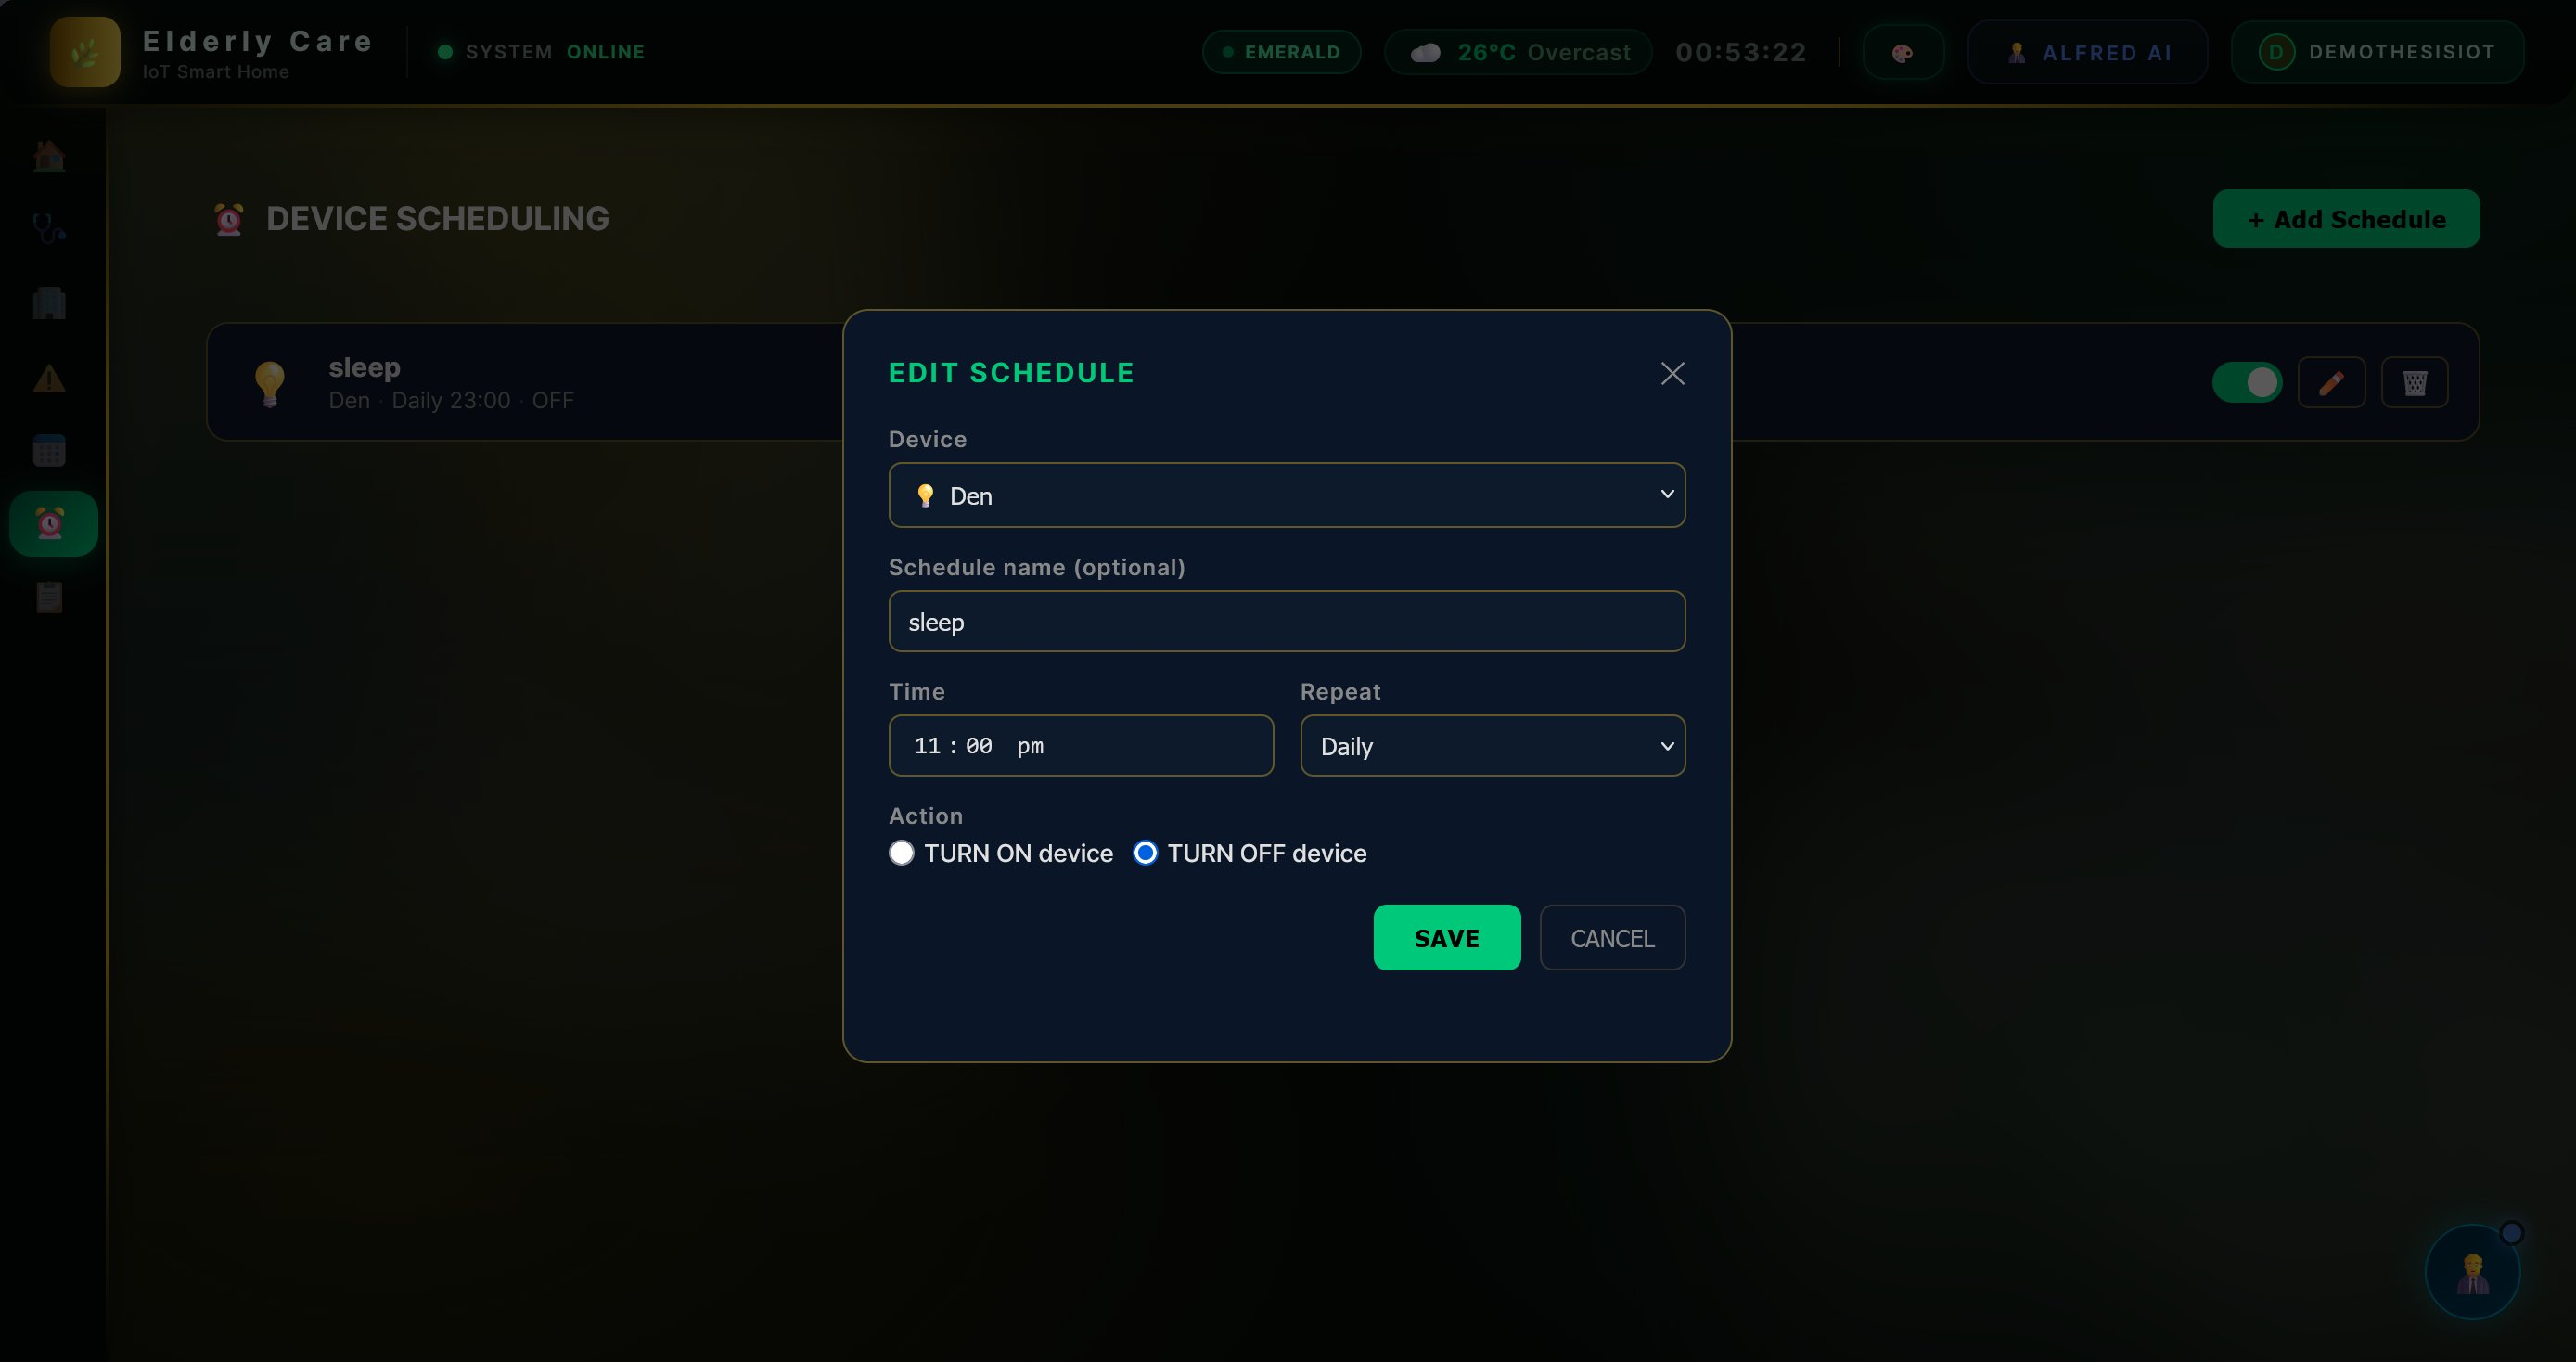
\includegraphics[width=0.92\textwidth]{images/web_scheduling.png}
\caption[Device Schedule sub-tab: cron-based device on/off control]{Device
         Schedule sub-tab (Care \& Schedule page, web dashboard). The
         \emph{Edit Schedule} dialog configures a daily \textit{sleep}
         schedule that turns the bedroom light (\texttt{Den}) off at 23:00;
         the saved schedule is listed behind the dialog with an enable/disable
         toggle and edit/delete controls. The dialog fields map directly to the
         \texttt{schedules} record (label, cron-derived time, repeat, and
         ON/OFF action) described in Section~\ref{subsec:device_scheduling}.}
\label{fig:web_scheduling}
\end{figure}

\subsection{Integration of Alfred AI Chat} \label{subsec:alfred_impl}

Alfred is exposed via three REST endpoints under \path{/api/ai/}: 
\texttt{POST /chat} (message with optional \texttt{mode} and \texttt{language}), \texttt{POST /analyze} (background AI analysis of sensor data) and \texttt{GET /status} (engine version and module availability). The design of the pipeline is described in Section~\ref{sec:alfred_method}.

Device-control requests must be confirmed by a mandatory two-step process: Alfred stores a pending action, prompts for user confirmation, and dispatches the MQTT command via \texttt{MqttPublisher.send\_device\_command()} only after affirmation. Mood-triggered suggestions (e.g. \textit{``nóng quá''} / ``it's too hot'') in multi-room deployments require room selection to avoid unintentional actuation.

Three Socket.IO events push Alfred output proactively: \texttt{ai\_mood} (environment suggestions on sensor threshold crossing), \texttt{ai\_advice} (wellness advice from heart-rate data), and \texttt{ai\_explain} (device action proposals with a \texttt{requires\_confirmation} flag rendered as a dismissible popup).

\FloatBarrier


\section{Results}
\label{sec:results}

\subsection{Hardware Prototype Validation}

The ESP32 firmware was compiled and deployed on a physical ESP32-WROOM-32 development board. The device connected to Wi-Fi reliably, published sensor telemetry every five seconds, and responded correctly to relay commands from both the web dashboard and the mobile application during testing.
The heart-rate readings from the Coospo~H6 arrived through the Python BLE bridge and were processed by the anomaly-detection pipeline without errors.

Figure~\ref{fig:pcb_prototype} shows the assembled prototype during a live
test session. The LCD status display reads \texttt{Wi:OK MQ:OK / D:ON Q:ON},
confirming active WiFi and MQTT broker connections with both relay channels
energised. A small DC fan is connected to Relay~1 as a representative
load device, demonstrating end-to-end control from the web dashboard.

\begin{figure}[htbp]
\centering
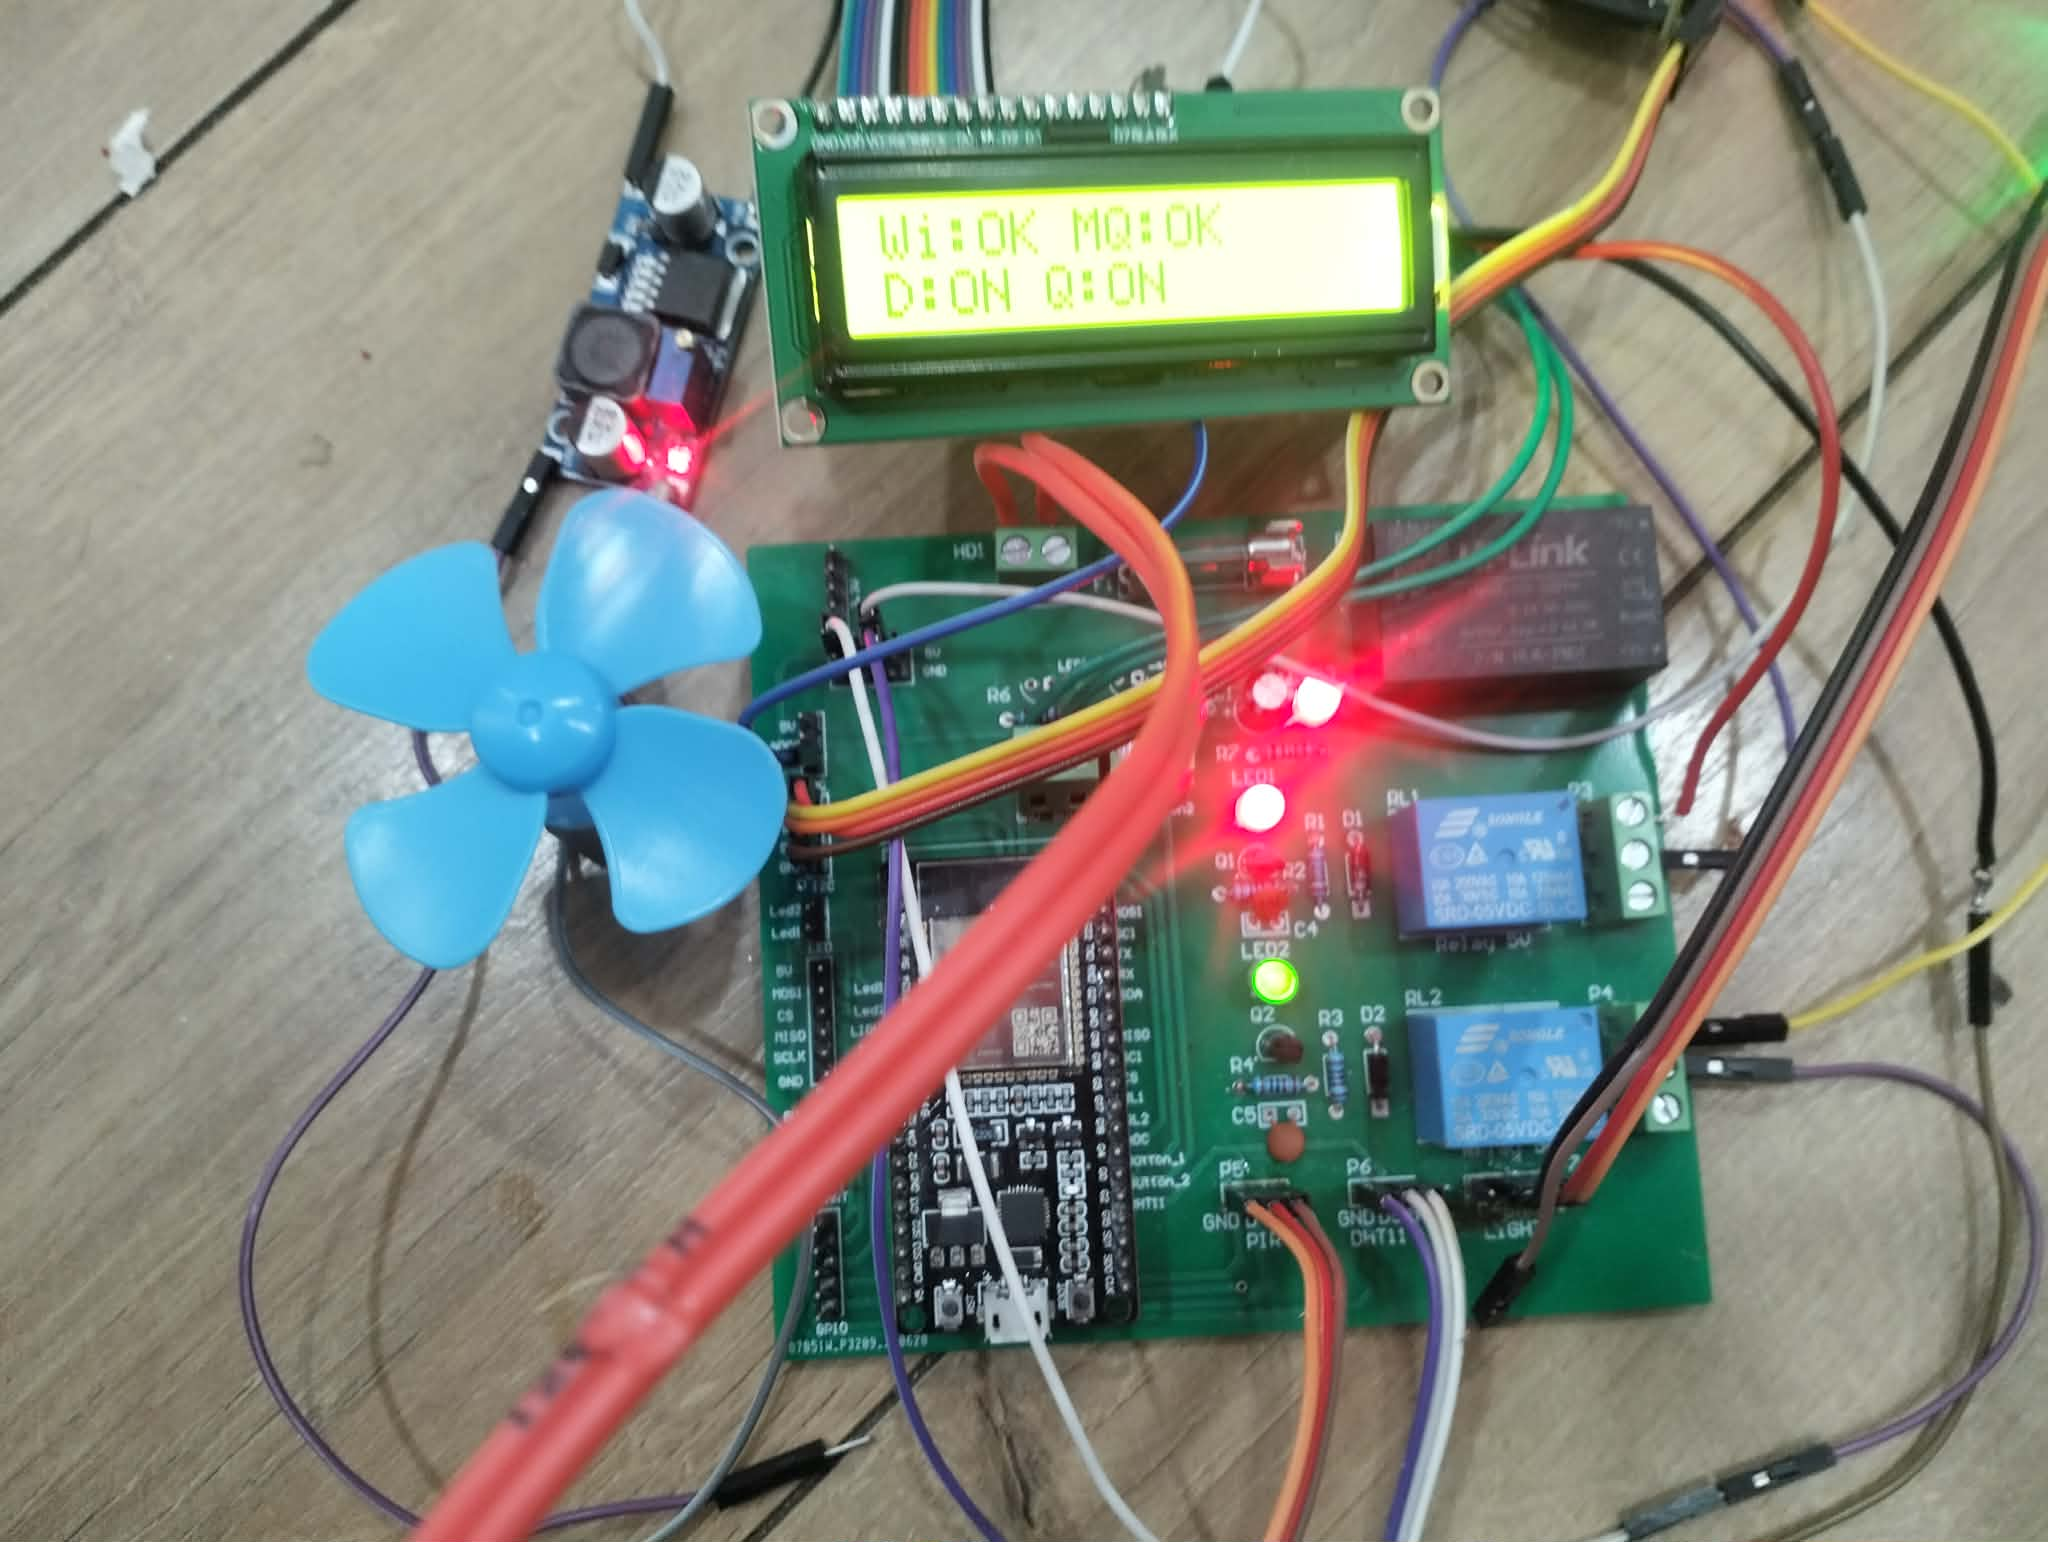
\includegraphics[width=0.82\textwidth]{images/pcb_prototype.jpg}
\caption[Assembled prototype board during a live test session]{Assembled prototype board during a live test session. The LCD reads
         \texttt{Wi:OK MQ:OK / D:ON Q:ON}: WiFi connected, MQTT broker
         connected, and both relay channels active. A DC fan is wired to
         Relay~1 as a representative controlled load. Red indicator LEDs
         confirm relay energisation; the green LED (LED2) indicates normal
         system operation.}
\label{fig:pcb_prototype}
\end{figure}

\subsection{Backend Validation Results}

Table~\ref{tab:backend_verify} summarises the reproducible checks performed
on the backend.

\begin{table}[H]
\centering
\caption{Backend validation results (April~2026)}
\label{tab:backend_verify}
\small
\begin{tabular}{lc}
\toprule
\textbf{Check} & \textbf{Outcome} \\
\midrule
Import diagnostics / editor errors            & Pass \\
Signed HttpOnly cookie auth                   & Pass \\
Rate-limit configuration                      & Pass \\
Ownership scoping (device / history)          & Pass \\
\bottomrule
\end{tabular}
\end{table}

All four checks passed. The first shows a clean module graph with no editor-level errors. The other three test the security path directly: signed-cookie auth, the rate limits, and per-user ownership scoping all behave as intended when actually probed, not just on paper.

Beyond the static checks, the device control path was also confirmed end-to-end. Each command follows a fixed route regardless of whether it comes from a manual dashboard toggle or an Alfred voice instruction: the request hits \texttt{POST /api/devices/control}, passes \texttt{@auth\_required}, and the backend publishes an MQTT command to the EMQX broker over TLS. The ESP32 picks it up on \texttt{home/control/\{code\}}, switches the relay, and publishes a confirmation to \texttt{home/status/\{code\}}. The backend MQTT listener then updates \texttt{device\_status} in the database and emits a Socket.IO \texttt{device\_status} event to the user's room, giving both the web dashboard and the Flutter client a live update without polling.





\subsection{Medication Reminder Runtime Flow}

The APScheduler background job queries \texttt{medicine\_reminders} once per minute and fires for any record whose \texttt{time\_of\_day} falls within a $\pm$1-minute window of the current time. When a reminder is due, the dispatcher sends an email to the caregiver's registered address and calls \texttt{AlertUseCase.create\_alert()}, which persists the alert and emits an \texttt{alert} Socket.IO event to every active session belonging to that user. The Flutter client surfaces this as an actionable notification banner; the web dashboard shows it as an informational toast. Once the caregiver taps \textbf{TAKEN}, the backend records \texttt{last\_taken\_on = today}, preventing any further dispatches for that reminder on the same calendar day.

If the reminder record carries an optional \texttt{notify\_email} field, the dispatch service adds it as a second recipient --- useful for family members or on-call staff who are not logged into the application but still need to be kept in the loop.









% ─────────────────────────────────────────────────────────────
\subsection{Heart-Rate Processing Pipeline}
\label{sec:hr_flow}

When a BLE reading arrives from the Coospo~H6 sensor, the MQTT callback invokes \texttt{monitor.on\_bpm\_update()}. Every reading is persisted unconditionally but throttled to one database write per 60 seconds, so the record always reflects the most recent value without flooding the table. In parallel, the HRV analyzer appends the reading to a 60-reading sliding window and broadcasts RMSSD, SDNN, and pNN50 metrics to the dashboard every 15 seconds --- these are companion metrics only and do not trigger alerts on their own.

Classification runs in two tiers. Rule-based thresholds fire first: readings at or above 130\,bpm are classified as \textit{emergency}, 100--129\,bpm as \textit{warning\_high}, and below 50\,bpm as \textit{warning\_low}. Readings that fall within the nominal zone are then passed to the Isolation Forest, which scales the BPM value with the fitted \texttt{anomaly\_hr\_scaler} before calling \texttt{predict()}. If the resolved risk level is anything other than normal, a 30-second cooldown since the most recent alert is checked. When the cooldown has elapsed, the backend emits a Socket.IO \texttt{hr\_alert} event to the user's room, creates a persistent alert record, and writes a forced database update with severity, risk level, and current HRV metrics attached. The design is described in Section~\ref{sec:anomaly_design}; the validation below confirms all stages execute correctly end-to-end.

The four-level risk classification scheme is defined in Table~\ref{tab:risk} (Section~\ref{subsec:risk_design}). Readings in the 50--99\,bpm range are labeled \textit{Normal}; under 50\,bpm is \textit{Caution}; 100--129\,bpm is \textit{Warning}; 130\,bpm and above is \textit{Critical}. An Isolation Forest outlier in the borderline zone (50--59 or 96--99\,bpm) is also promoted to \textit{Caution}; outliers in the clearly normal zone (60--95\,bpm) are suppressed to keep false positive alerts low. Each risk level gets a distinct colour on the chart (green, yellow, orange, red); Critical events also trigger an audio chime and an in-app banner.

\subsection{Alert Panel and Caregiver Acknowledgement}

When a threshold is breached or Isolation Forest outlier occurs, the backend logs an alert and emits a Socket.IO \texttt{alert} event. Web clients show a toast with audio chime for critical alerts. Mobile shows an in-app banner. The Alert Management panel displays alerts in reverse-chronological order; caregivers can ACK, delete, or bulk-clear entries. Six mute scopes (by sensor type, keyword, or device code) filter out non-actionable noise.

Elderly users can trigger an SOS emergency through the Alfred chat interface without leaving the page. Alfred's pipeline runs a distress keyword detector at the highest priority. Recognised phrases include ``cứu tôi'', ``cứu với'', ``không thở được'', ``đau ngực'', ``tôi bị ngã'', and ``SOS''. Alfred then: (1) clears pending actions, (2) creates a critical alert (\texttt{device\_code = "SOS"}), (3) sends an emergency email to caregivers, and (4) replies with local emergency numbers. Detection works in all chat modes without confirmation.

A dedicated \textbf{SOS button} in the chat input bar opens a modal for voice notes (up to 30\,s, via \texttt{MediaRecorder}) and optional text. The modal respects the VI/EN language toggle. On submission, the backend creates the alert and sends an HTML email with the voice note attached. XSS is prevented via \texttt{html.escape()}. A confirmation message appears in chat history.









% ─────────────────────────────────────────────────────────────
\subsection{Web Dashboard Validation}
\label{sec:web_impl}

Table~\ref{tab:web_verify} summarises the Vite build and feature checks
performed on the web dashboard.

\begin{table}[H]
\centering
\caption{Web dashboard validation results}
\label{tab:web_verify}
\small
\begin{tabularx}{\textwidth}{@{}>{\raggedright\arraybackslash}X c@{}}
\toprule
\textbf{Check} & \textbf{Outcome} \\
\midrule
Vite production build              & Pass \\
Auth storage hardening             & Pass \\
Socket room join flow              & Pass \\
Alert ACK and delete               & Pass \\
Medicine reminders CRUD            & Pass \\
Admin panel role gating            & Pass \\
Map device position stability      & Pass \\
Alfred patient-name greeting       & Pass \\
\bottomrule
\end{tabularx}
\end{table}

The home dashboard (Figure~\ref{fig:method_dashboard_layout}) presents a
sensor strip at the top (live Heart Rate, weather temperature, schedule and alert
counters) followed by five navigation module cards --- Health Monitor,
Rooms \& Devices, Care \& Schedule, Daily Report, and Alerts \& SOS ---
each linking directly to its full-detail page.

The \textbf{Health Monitor} page (Figure~\ref{fig:web_health_overview}) provides
the full biometric detail. The Bio-Metrics panel shows a sensor card for Heart
Rate alongside a risk-level indicator ring and an Alfred AI diagnosis summary. The Live Heart-Rate Monitor panel renders a
real-time BPM waveform with risk-level colour coding derived from the Isolation
Forest anomaly detector.

\begin{figure}[htbp]
\centering
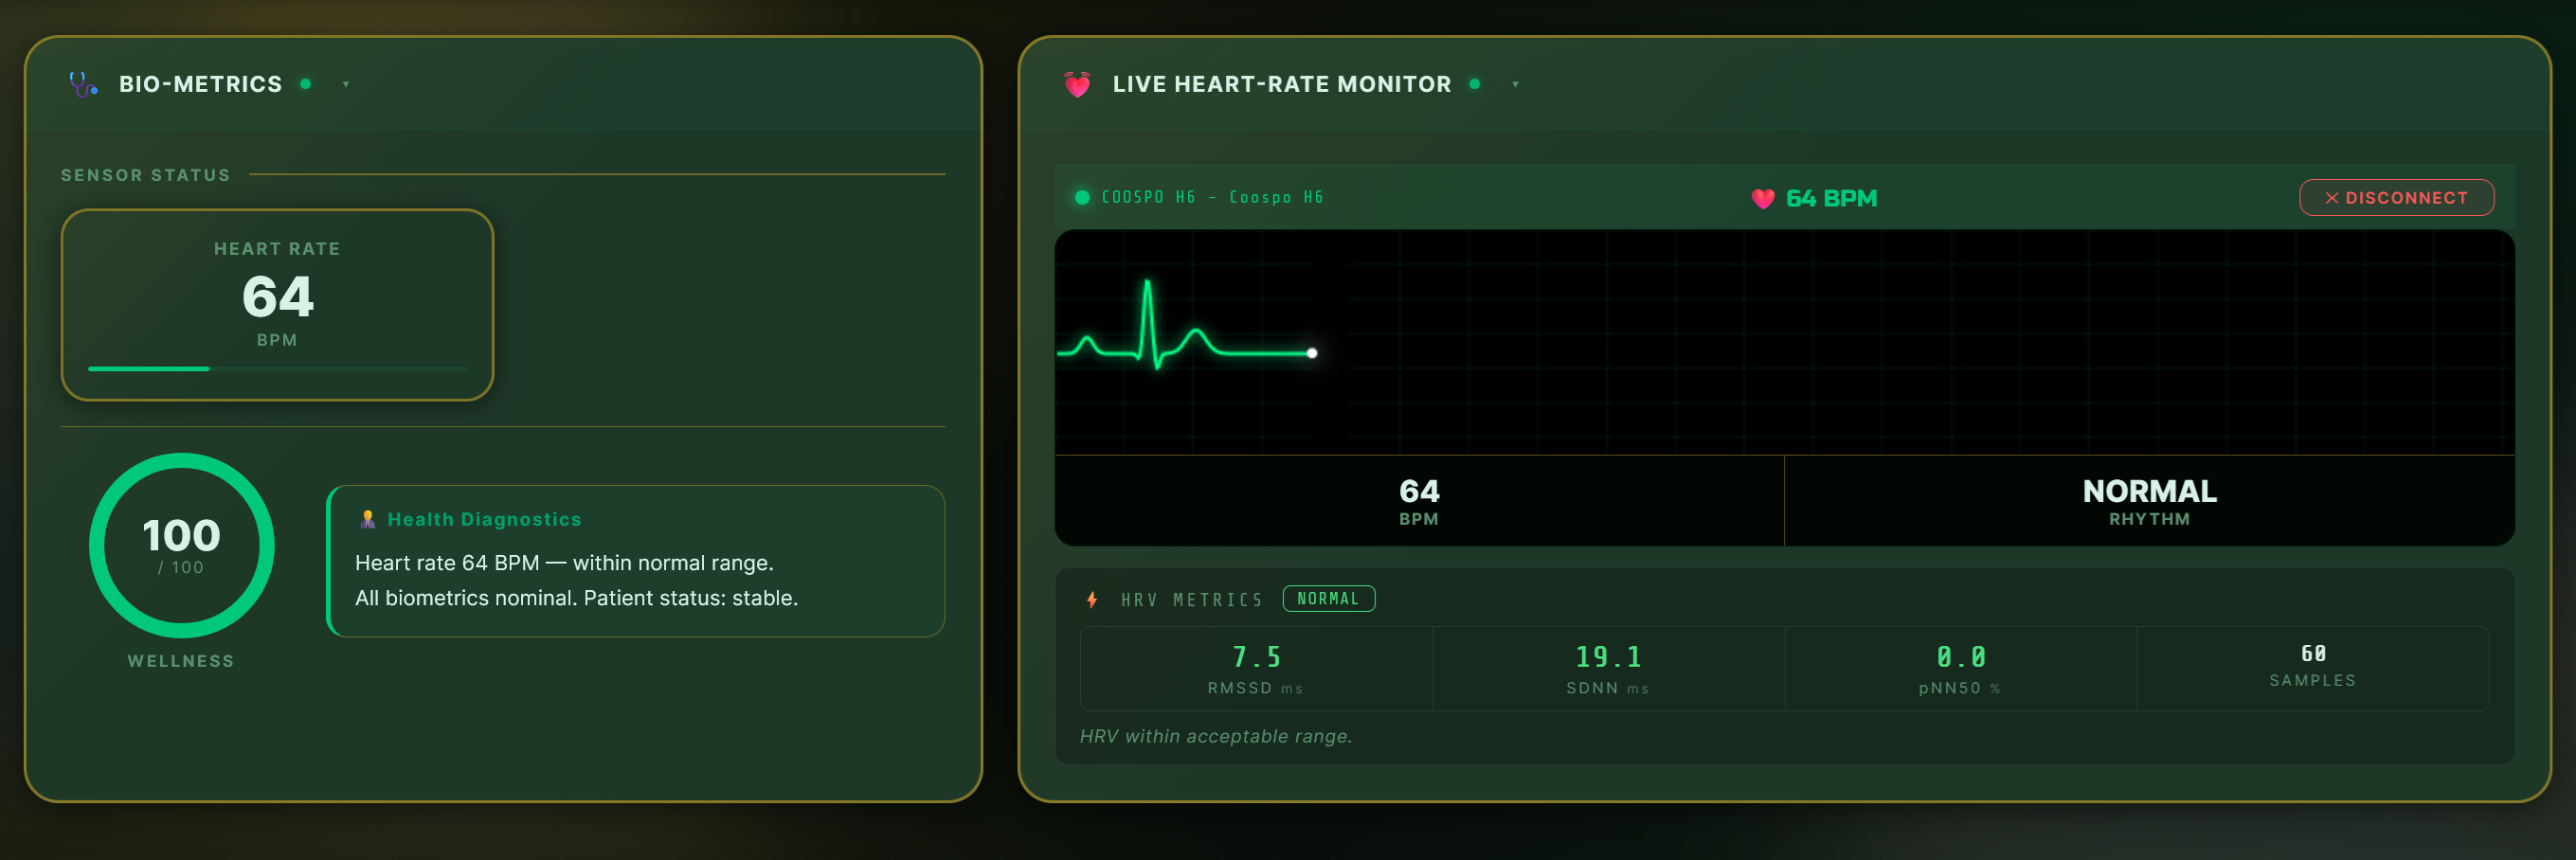
\includegraphics[width=0.92\textwidth]{images/web_health.png}
\caption[Health Monitor page overview]{Health Monitor page: Bio-Metrics panel (Heart Rate 64\,BPM, risk-level indicator, Alfred AI diagnosis) alongside Live Heart-Rate Monitor with real-time BPM waveform and NORMAL risk status.}
\label{fig:web_health_overview}
\end{figure}

The \textbf{Alert Management} page (Figure~\ref{fig:alerts_detail}) lists all
system events with severity filters (ALL / UNREAD / CRITICAL / WARNING), device
and time filters, and bulk-clear controls. The alert toolbar supports six
user-scoped mute modes (all alerts, heart-rate, light, fan/AC, custom keyword,
exact device code) persisted to the backend for cross-session consistency.

\begin{figure}[H]
\centering
\begin{subfigure}[t]{0.48\textwidth}
    \centering
    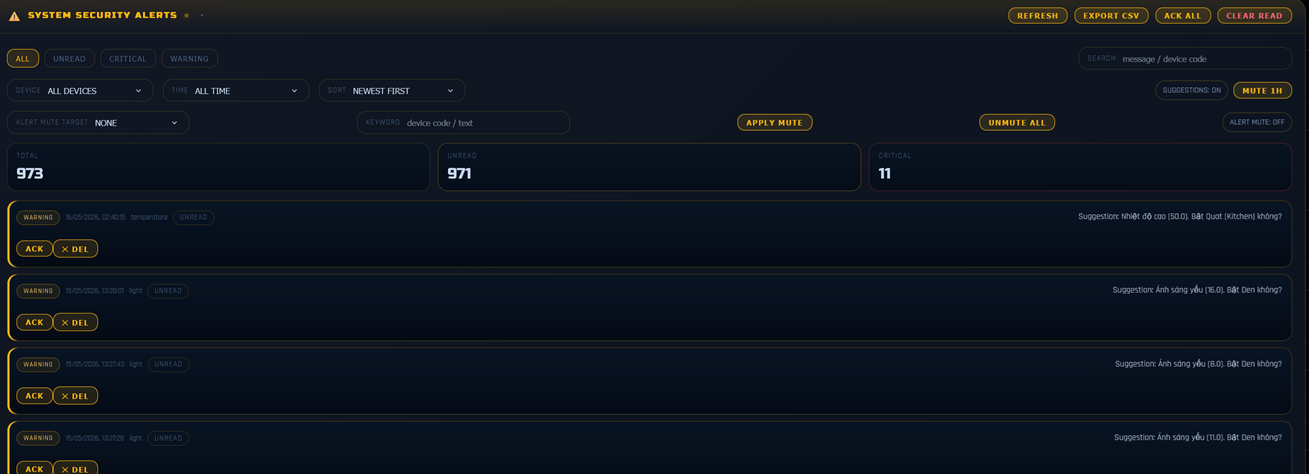
\includegraphics[width=\textwidth]{images/fig_alerts_system_interface.png}
    \caption{Alert list: severity filters (ALL/UNREAD/CRITICAL/WARNING), device
             and time filters, alert mute controls, and real-time suggestion log.}
    \label{fig:alerts_system_interface}
\end{subfigure}
\hfill
\begin{subfigure}[t]{0.48\textwidth}
    \centering
    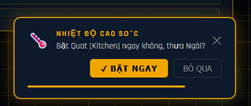
\includegraphics[width=\textwidth]{images/fig_environmental_alert_confirmation.png}
    \caption{Environmental alert confirmation dialog.}
    \label{fig:env_alert_confirm}
\end{subfigure}
\caption{Alert Management page.}
\label{fig:alerts_detail}
\end{figure}

The \textbf{Rooms \& Deployment} page (Figure~\ref{fig:web_admin_screens})
has two tabs. The ROOMS tab shows room records and which devices belong to each room;
the DEVICES tab lists all registered devices with their current online status
and MQTT topic. Below the tabs, a floor-plan canvas lets the caregiver
upload a blueprint image and draw room boundaries by clicking polygon vertices.
Each polygon is then given a name and a colour.

Figure~\ref{fig:floorplan_editor_full} shows the two steps of that process.
After closing a polygon the Zone Designation dialog
(Figure~\ref{fig:map_zone_dialog}) asks for a room name and a zone colour
before saving. The finished result (Figure~\ref{fig:rooms_floorplan_editor_detail})
shows the floor plan with all named zones drawn on top, so the caregiver
can see at a glance which device is in which room.

\begin{figure}[htbp]
\centering
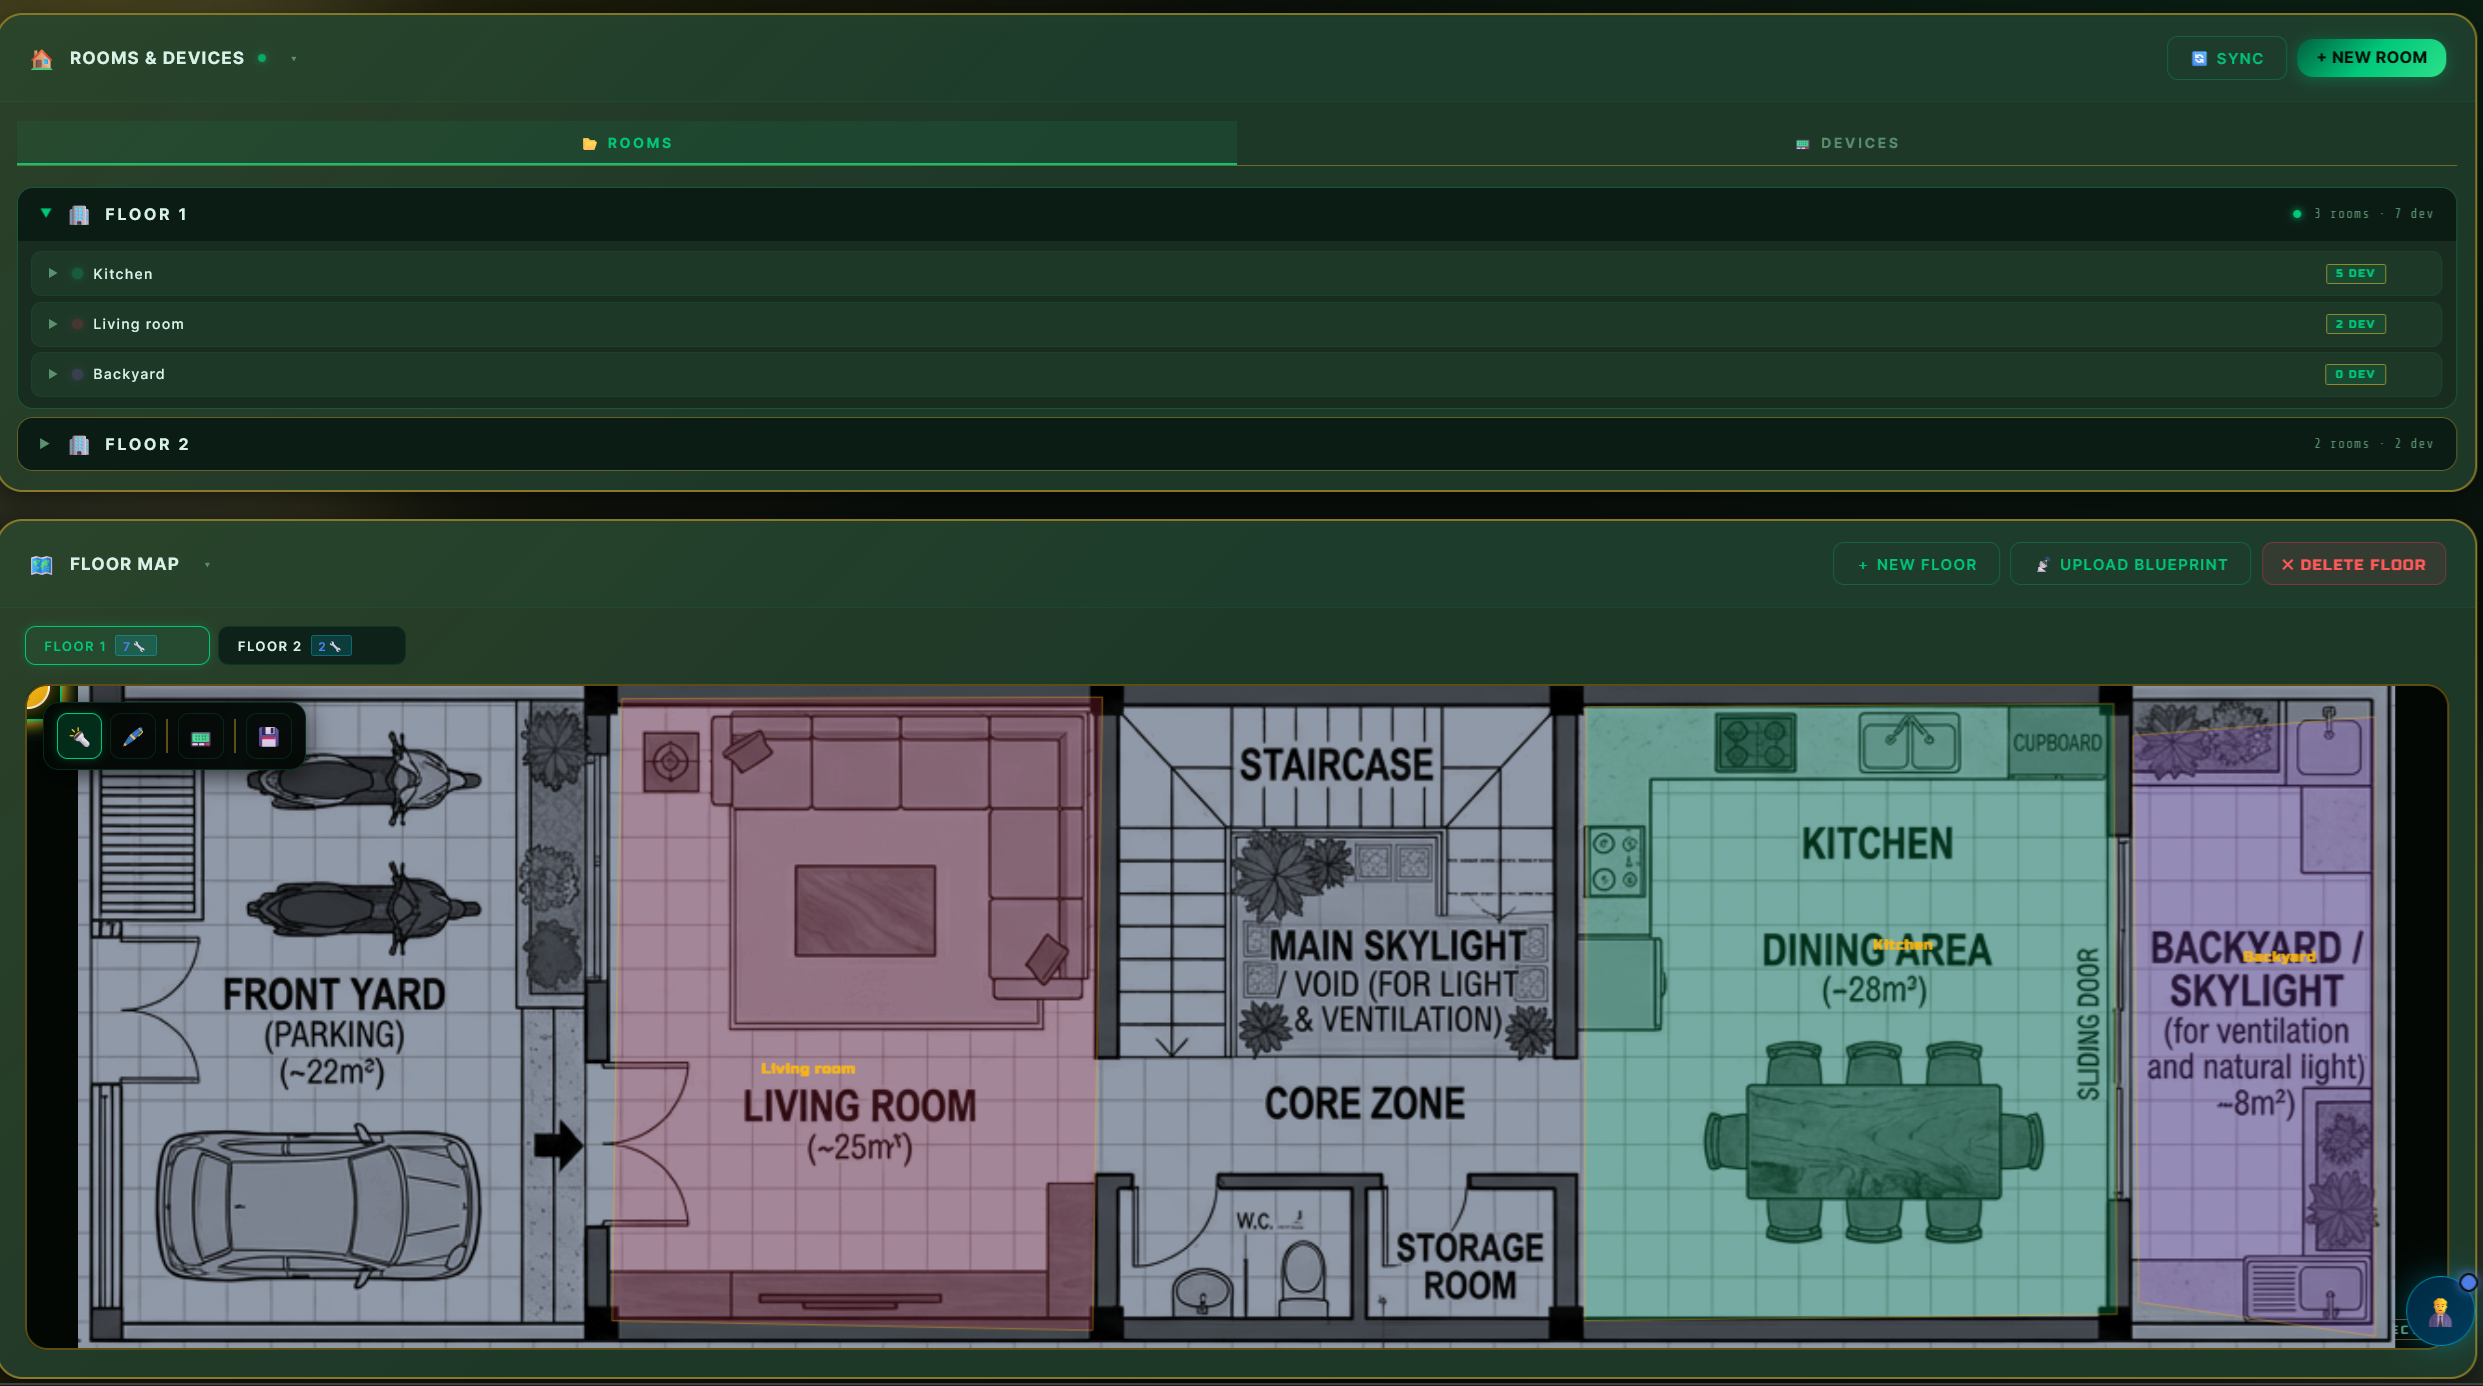
\includegraphics[width=0.92\textwidth]{images/web_rooms.png}
\caption[Rooms \& Deployment page]{Rooms \& Deployment page: ROOMS/DEVICES tabs and floor-plan canvas
         editor awaiting blueprint upload.}
\label{fig:web_admin_screens}
\end{figure}

\begin{figure}[H]
\centering
\begin{subfigure}[t]{0.42\textwidth}
    \centering
    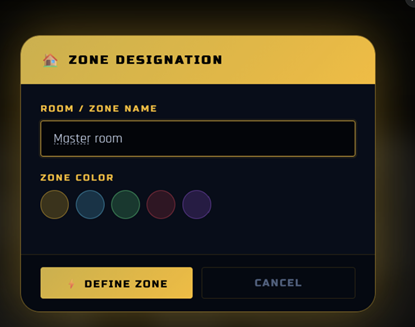
\includegraphics[width=\textwidth,keepaspectratio]{images/fig_rooms_floor_plan_editor.png}
    \caption{Zone Designation dialog: naming a room and selecting its zone colour
             before the polygon is committed to the database.}
    \label{fig:map_zone_dialog}
\end{subfigure}
\hfill
\begin{subfigure}[t]{0.52\textwidth}
    \centering
    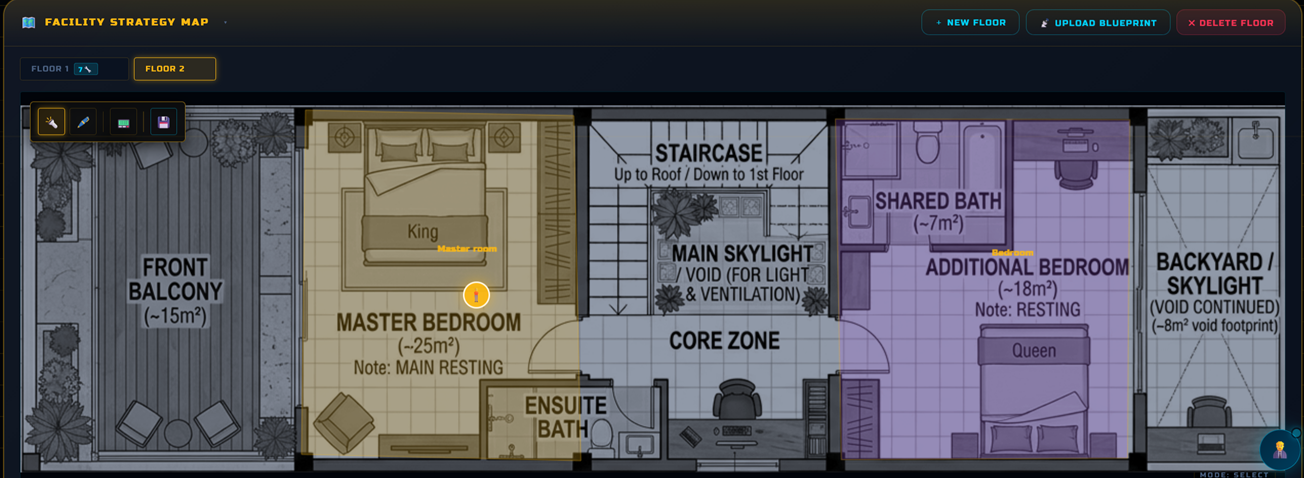
\includegraphics[width=\textwidth,keepaspectratio]{images/fig_map_zone_dialog.png}
    \caption{Floor-plan overlay: facility room map showing traced polygon boundaries
             across multiple zones (Front Balcony, Master Bedroom, Core Zone, etc.).}
    \label{fig:rooms_floorplan_editor_detail}
\end{subfigure}
\caption[Floor-plan editor workflow]{Floor-plan editor workflow: (a) zone definition dialog for naming and
         colour-coding a room polygon; (b) resulting overlay on the uploaded
         floor-plan image with live room boundaries.}
\label{fig:floorplan_editor_full}
\end{figure}

Table~\ref{tab:web_screens_result} summarises all seven web dashboard views.

{\small
\begin{longtable}{l p{11cm}}
\caption{Web dashboard view summary}
\label{tab:web_screens_result} \\
\toprule
\textbf{View} & \textbf{Key Features} \\
\midrule
\endfirsthead
\multicolumn{2}{c}{{\tablename\ \thetable{} -- continued from previous page}} \\
\toprule
\textbf{View} & \textbf{Key Features} \\
\midrule
\endhead
\midrule
\multicolumn{2}{r}{{Continued on next page}} \\
\endfoot
\bottomrule
\endlastfoot
Main Dashboard        & Stat strip (live BPM, weather temperature, schedule count, alerts count); AI Health Analysis panel (risk-level ring + Alfred AI diagnosis); Recent Alerts, Today's Schedule, and Quick Devices summary widgets \\[3pt]
Health Monitor        & BPM time-series, vitals summary, Isolation Forest risk flags, mood label \\[3pt]
Alert Management      & Severity filters, acknowledge/dismiss, bulk-clear, user-scoped mute by target (all / heart-rate / light / fan-AC / custom / exact device code) \\[3pt]
Care \& Schedule      & Two sub-tabs: \textit{Care \& Reminders} — Google Calendar-style Day/Week/Month views with event types (Medicine/Activity/Appointment/Note), mini-calendar sidebar, medicine adherence progress bar; \textit{Device Schedule} — cron-based timed relay actions \\[3pt]
Health Report         & Daily report (medicine adherence, schedule, today's alerts) and Weekly report (HR vital signs, AI assessment, alert severity breakdown, clinical profile); live panel with progress bars \\[3pt]
Room Configuration    & Polygon draw tool, floor tabs, device assignment, real-time sync \\[3pt]
Care Staff            & Caregiver CRUD, patient assignment, role-gated admin access \\
\end{longtable}
}


\subsection{Care and Schedule Management Page}

The page is organised into two sub-tabs. In the \textbf{Care \& Reminders} sub-tab, all event categories (activities, appointments, notes, and medicine reminders)
are persisted to the backend via \texttt{/api/care-events} and
\texttt{/api/reminders} and rendered correctly in the calendar interface
(Figure~\ref{fig:care_day_view}). The Device Schedule sub-tab exposes the
cron-based timed relay interface described in
Section~\ref{subsec:device_scheduling}.

\begin{figure}[htbp]
\centering
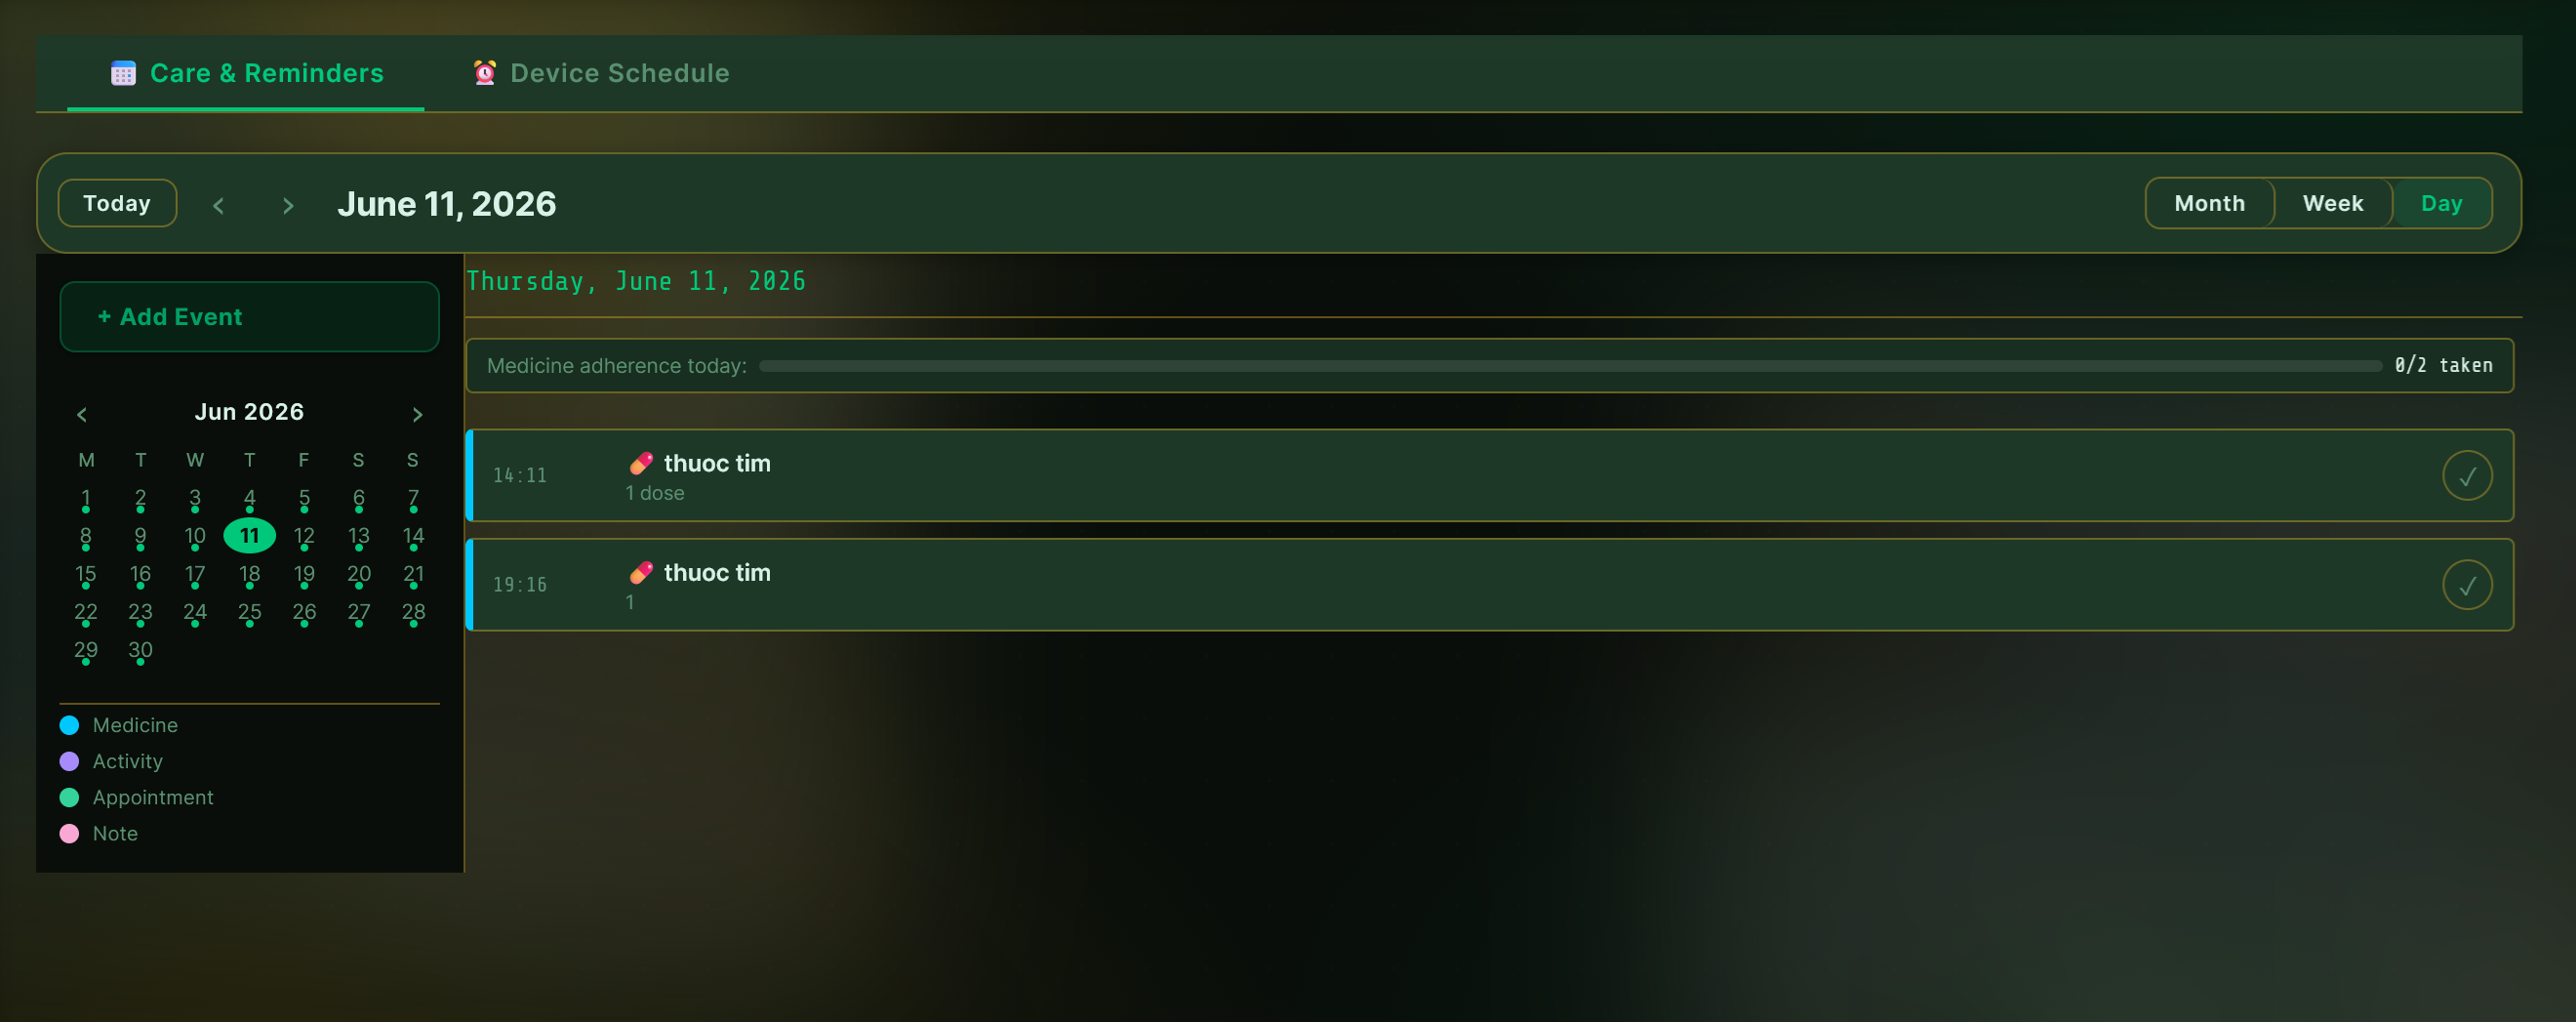
\includegraphics[width=0.90\textwidth]{images/web_care_day.png}
\caption[Care \& Schedule page --- Day view (June 2026)]{Care \& Schedule page --- Day view (June 11, 2026): timeline listing of medicine events for the selected day (\textit{thuốc tim} at 14:11 and 19:16), with a medicine adherence progress bar (0/2 taken) at the top. Left sidebar provides an \textbf{Add Event} button, mini monthly calendar for date navigation, and a colour-coded legend (Medicine, Activity, Appointment, Note).}
\label{fig:care_day_view}
\end{figure}

\subsection{Health Report Panel}

The Health Report panel (Figure~\ref{fig:method_health_report}) shows a
summary of recent heart-rate data in either a daily or weekly view.
The top of the panel displays summary numbers from the stored BPM history;
in the captured session these were Average BPM 74 and Maximum BPM 98,
which confirms that heart-rate readings are reaching the report layer correctly.
The export button triggers \texttt{window.print()}, producing a
printer-ready PDF. Both the Daily and Weekly views rendered and exported
without error during testing.

\subsection{Alfred Rule Engine in Practice}
\label{subsec:alfred_rule_result}

The Alfred implementation described in Section~\ref{subsec:alfred_impl} was validated across all three inference modes. All 19 intent groups fired correctly on representative trigger phrases in both Vietnamese and English. Unrecognised utterances resulted in the expected structured fallback response. The complete intent taxonomy is available in Appendix~\ref{app:alfred_keywords}.

The two-step device confirmation flow was verified end-to-end: issuing \textit{``bật đèn''} (turn on the light) caused Alfred to store a pending action and return a confirmation prompt; the MQTT command was dispatched via \texttt{MqttPublisher.send\_device\_command()} only after the user confirmed. Cancelling the prompt left the device state unchanged.

Mood-trigger phrases such as \textit{``nóng quá''} correctly prompted room selection followed by a separate confirmation step before actuation, preventing accidental commands in multi-room scenarios.

Beyond text input, Alfred also accepts spoken commands. The voice input panel (Figure~\ref{fig:alfred_voice}) transcribes Vietnamese speech in real time via the Web Speech API and forwards the resulting transcript to the \texttt{/api/ai/chat} endpoint unchanged, so the same intent-matching logic applies regardless of whether the user typed or spoke the phrase.

\begin{figure}[H]
\centering
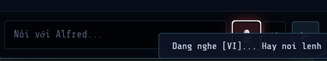
\includegraphics[width=0.52\textwidth]{images/fig_voice_input_microphone.png}
\caption[Voice input panel (locale \texttt{vi\_VN})]{Voice input panel: microphone activation button and real-time
         speech-to-text transcription (locale \texttt{vi\_VN}).}
\label{fig:alfred_voice}
\end{figure}

% ─────────────────────────────────────────────────────────────
\subsection{Mobile Application Validation}
\label{sec:mobile_impl}

Eight screens are provided: six via a bottom navigation bar (CONTROL,
ROUTINES, ALFRED, HEALTH, ALERTS, MAP) plus Settings and Login.
The mobile client consumes the same REST API and Socket.IO endpoints as
the web dashboard; functional parity is by design. Two screens differ in
interaction model from their web counterparts and are shown in
Figure~\ref{fig:mobile_result_screens}: the ALERTS screen delivers
notifications as a badge counter rather than an overlay popup, and the
ROUTINES screen lists scheduled medicines with a \textbf{TAKEN} button
to record adherence. The MAP screen (Figure~\ref{fig:mobile_map_screen})
is read-only on mobile; floor-plan editing is performed on the web
dashboard.

\begin{figure}[H]
\centering
\begin{subfigure}[t]{0.42\textwidth}
    \centering
    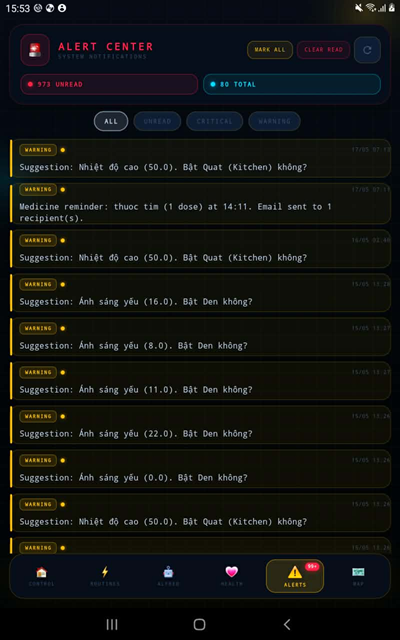
\includegraphics[width=\textwidth,height=0.38\textheight,keepaspectratio]{images/mobile_alerts.png}
    \caption{Alerts --- badge counter, severity filter, real-time feed}
    \label{fig:mobile_alerts}
\end{subfigure}\hfill
\begin{subfigure}[t]{0.42\textwidth}
    \centering
    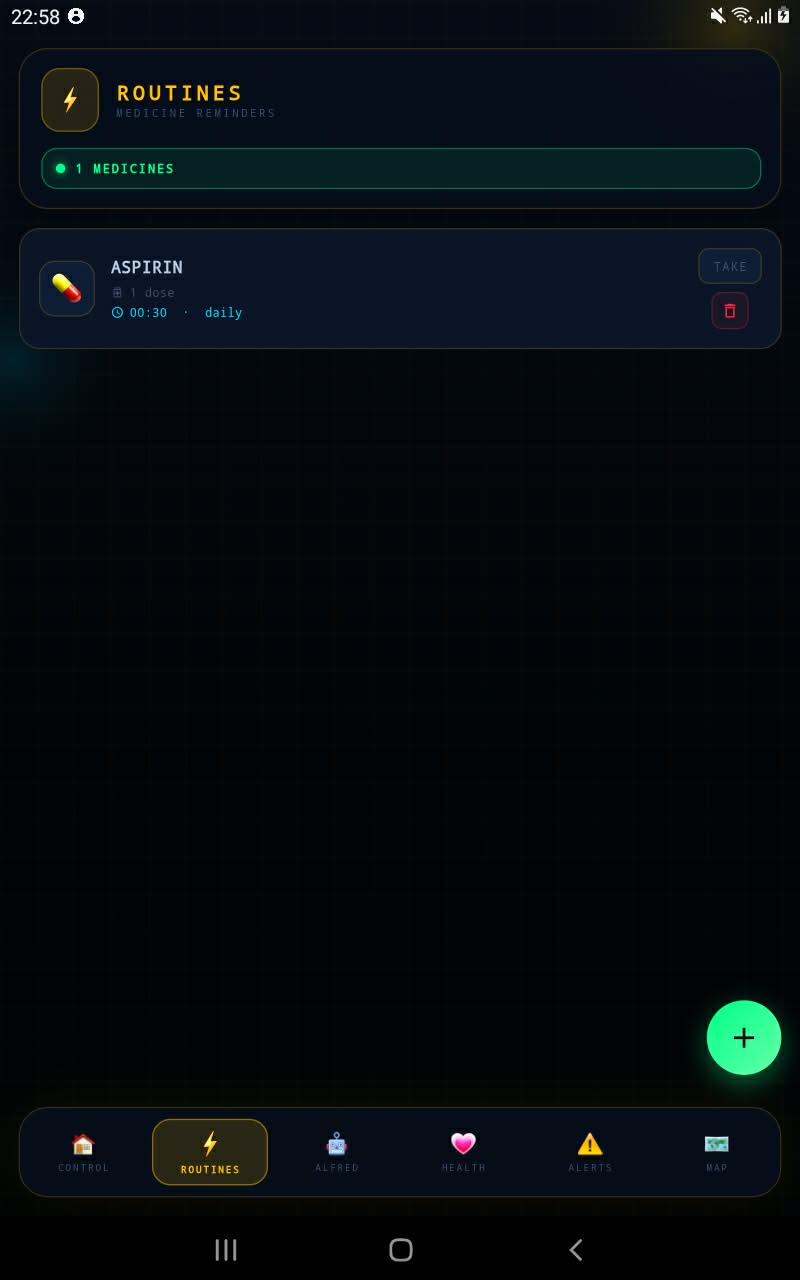
\includegraphics[width=\textwidth,height=0.38\textheight,keepaspectratio]{images/mobile_routines.png}
    \caption{Routines --- medicine schedule, TAKEN action}
    \label{fig:mobile_routines}
\end{subfigure}
\caption[Mobile application: Alerts and Routines screens]{Mobile application: Alerts screen (badge-based, no overlay popup)
         and Routines screen (medicine adherence). Both differ from their
         web counterparts in interaction model.}
\label{fig:mobile_result_screens}
\end{figure}

\begin{figure}[H]
\centering
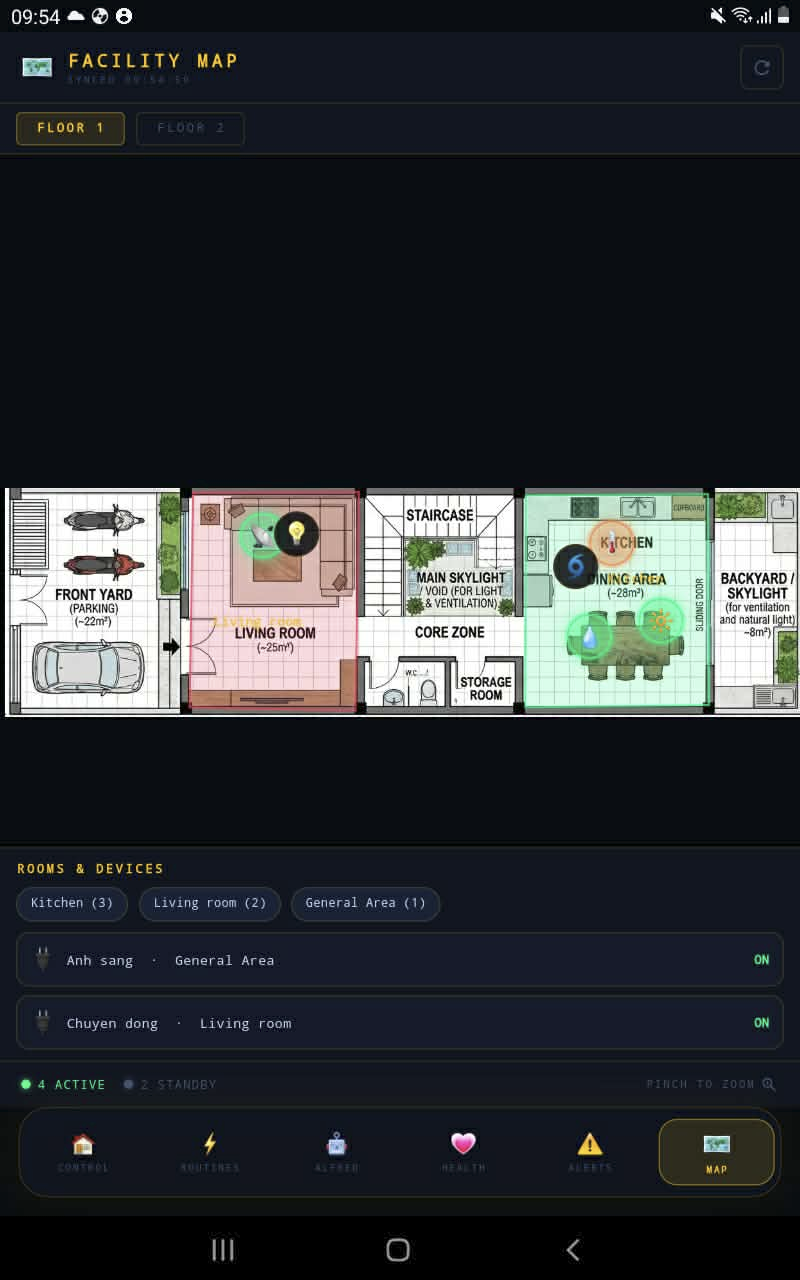
\includegraphics[width=0.52\textwidth]{images/mobile_map.png}
\caption[Mobile Map screen: floor-plan overlay]{Mobile Map screen: floor-plan overlay with room polygons and
         live device status markers. Read-only on mobile; layout editing
         is performed on the web dashboard.}
\label{fig:mobile_map_screen}
\end{figure}

During developer testing, all eight screens were manually navigated and confirmed functional on Android. All shared features with the web dashboard were confirmed to have functional parity.
Table~\ref{tab:mobile_verify} lists the static-analysis and test outcomes.

\begin{table}[H]
\centering
\caption{Mobile application validation results}
\label{tab:mobile_verify}
\small
\begin{tabularx}{\textwidth}{@{} >{\raggedright\arraybackslash}p{4.2cm} >{\centering\arraybackslash}p{1.6cm} >{\RaggedRight\arraybackslash}X @{}}
\toprule
\textbf{Check} & \textbf{Result} & \textbf{Notes} \\
\midrule
\texttt{flutter analyze}         & Pass & No issues after cleanup \\
Secure token storage             & Pass & \texttt{flutter\_secure\_storage} verified \\
Android network posture          & Pass & Cleartext disabled outside dev config \\
HTTPS / LAN dev flag             & Pass & Compile-time \texttt{--dart-define} \\
\bottomrule
\end{tabularx}
\end{table}

% ─────────────────────────────────────────────────────────────
\subsection{End-to-End Scenario Validation}
\label{sec:validation_scenarios}

Ten deterministic end-to-end scenarios were executed on the running system
with the full hardware stack active. All scenarios completed successfully, confirming correct behaviour
across all system layers (Table~\ref{tab:validation_scenarios}).

\begin{table}[H]
\centering
\caption[System validation scenarios]{System validation scenarios (developer self-test walkthrough; all ten scenarios completed without error on the running system)}
\label{tab:validation_scenarios}
\small
\begin{tabularx}{\textwidth}{@{}c p{2.7cm} X X@{}}
\toprule
\textbf{ID} & \textbf{Scenario} & \textbf{Action / Trigger} & \textbf{Expected Outcome} \\
\midrule
V1 & Device toggle via web & POST \path{/api/devices/control} with valid token & MQTT published; HTTP 200 \\[3pt]
V2 & Device toggle via mobile & Toggle switch in Flutter Control tab & Same MQTT publish as V1; UI updates via Socket.IO \\[3pt]
V3 & Anomaly alert trigger & Inject BPM = 145 via MQTT & Alert stored; Socket.IO event emitted \\[3pt]
V4 & Authentication check & Access protected API without token & HTTP 401 returned \\[3pt]
V5 & Rate limiting & Exceed 10 requests/minute & HTTP 429 with Retry-After header \\[3pt]
V6 & Alfred command & Chat: ``turn on the light'' & Alfred proposes action and asks confirmation; command executes after user affirms \\[3pt]
V7 & MQTT reconnect & Simulated broker disconnect & Re-subscription successful; data flow restored \\[3pt]
V8 & Room layout persistence & Save polygon via API & Data persisted and reflected on mobile map (Figure~\ref{fig:mobile_map_screen}) \\[3pt]
V9 & Reminder scheduling & Create medicine reminder via API & Triggered at scheduled time \\[3pt]
V10 & Alert cleanup & Delete read alerts via API & All acknowledged alerts removed \\
\bottomrule
\end{tabularx}
\end{table}

\chapter{DISCUSSION AND EVALUATION}

Three threads run through this chapter: a quantitative evaluation of the anomaly detection model, a cross-dimension analysis of system performance, and a mapping of the findings back to the three research questions from Chapter~1.

% ─────────────────────────────────────────────────────────────
\section{Anomaly Detection Model Evaluation}
\label{sec:ml_validation}

\subsection{Training Dataset Composition}

Table~\ref{tab:train_composition} lists all data used in the anomaly
detection pipeline, broken down by split and source.

The clinical data comes from the UCI Heart Disease Dataset~\cite{UCIHeartDisease1988}, a Kaggle release described as pooling records from four hospital sites (Cleveland, Hungary, Switzerland, VA~Long~Beach) totalling 1\,025 rows. Running \texttt{pandas.DataFrame.duplicated()} revealed that 723 of those rows are identical copies, leaving only 302 truly distinct records --- suggesting the multi-site collection largely replicates the well-known 303-patient Cleveland cohort rather than adding independent observations. The training pipeline does not apply explicit deduplication, so the 499 target=0 (healthy) rows drawn from the full CSV are used as-is; the duplicate Cleveland records therefore appear multiple times in training and inflate the effective weight of that cohort. This is acknowledged as a data-quality limitation in Section~\ref{sec:discussion_limitations}.

A second constraint is that the dataset records \texttt{thalach} --- peak HR achieved during a treadmill stress test --- rather than resting HR. Resting HR was approximated by scaling: $\texttt{thalach} \times \mathcal{U}(0.55,\,0.65)$, drawing the factor uniformly from $[0.55,\,0.65]$ to bring exercise-peak values into a plausible resting range. The scaling has no clinical basis and is the primary acknowledged limitation of this dataset; see Section~\ref{sec:discussion_limitations}.

The 1\,700 synthetic samples were added specifically to address a gap this conversion leaves open. Because all UCI readings originate from a supervised exercise protocol, none of them capture the lower HR values normal for an elderly person asleep at night (roughly 50--74\,bpm). Without these samples, early testing showed the model flagging normal sleep-time bradycardia as anomalies, so the synthetic night-time readings were added to push the decision boundary to a more realistic lower edge.

\begin{table}[H]
\centering
\caption[Data sources for the anomaly detection pipeline]{Data sources for the heart-rate anomaly detection pipeline.
  \emph{Production model} (\texttt{tune\_and\_retrain\_anomaly.py}) uses all data in the
  Production column; the \emph{Evaluation benchmark} (\texttt{benchmark/anomaly/eval\_benchmark\_model.py})
  uses only the UCI 80/20 split with no synthetic samples.}
\label{tab:train_composition}
\footnotesize
\setlength{\tabcolsep}{5pt}
\renewcommand{\arraystretch}{1.3}
\begin{tabular}{@{}
  l
  >{\raggedright\arraybackslash}p{3.2cm}
  r
  r
  >{\raggedright\arraybackslash}p{5.4cm}
@{}}
\toprule
\textbf{Split} & \textbf{Source} & \textbf{Samples} & \textbf{HR (bpm)} & \textbf{Notes} \\
\midrule
\multicolumn{5}{@{}l}{\textit{Production model training (contamination\,=\,0.020, $n\_estimators$\,=\,300)}} \\[2pt]
Train
  & Generated (code)
  & 1\,700 & 50--91
  & Night: 50--74\,bpm; daytime: 60--91\,bpm.
    Covers sleep-time HR absent from UCI. \\[3pt]
  & UCI healthy (target\,=\,0) \cite{UCIHeartDisease1988}
  & 499 & 40--123
  & All healthy records; resting HR estimated as
    $\texttt{thalach} \times \mathcal{U}(0.55,0.65)$. \\
\cmidrule(l){2-5}
  & \textbf{Production total} & \textbf{2\,199} & & \\
\midrule
\multicolumn{5}{@{}l}{\textit{Evaluation benchmark (80/20 UCI split, contamination\,=\,0.10, $n\_estimators$\,=\,200)}} \\[2pt]
Train
  & UCI healthy 80\,\% \cite{UCIHeartDisease1988}
  & 399 & 40--123
  & Same thalach estimation; no synthetic data used. \\[3pt]
Test
  & UCI healthy held-out 20\,\%
  & 100 & 40--123
  & Labelled \emph{normal}. \\[3pt]
  & UCI diseased (target\,=\,1) \cite{UCIHeartDisease1988}
  & 526 & varies
  & $\texttt{thalach} \times \mathcal{U}(1.10,1.25)$;
    labelled \emph{anomaly}. \\
\cmidrule(l){2-5}
  & \textbf{Eval test total} & \textbf{626} & & \\
\bottomrule
\end{tabular}
\end{table}

Figure~\ref{fig:if_eval_flow} summarises the end-to-end data flow of this
benchmark, from the raw UCI and synthetic sources through the 80/20 split and
contamination selection to the final evaluation on the shared held-out test set.

\begin{figure}[H]
\centering
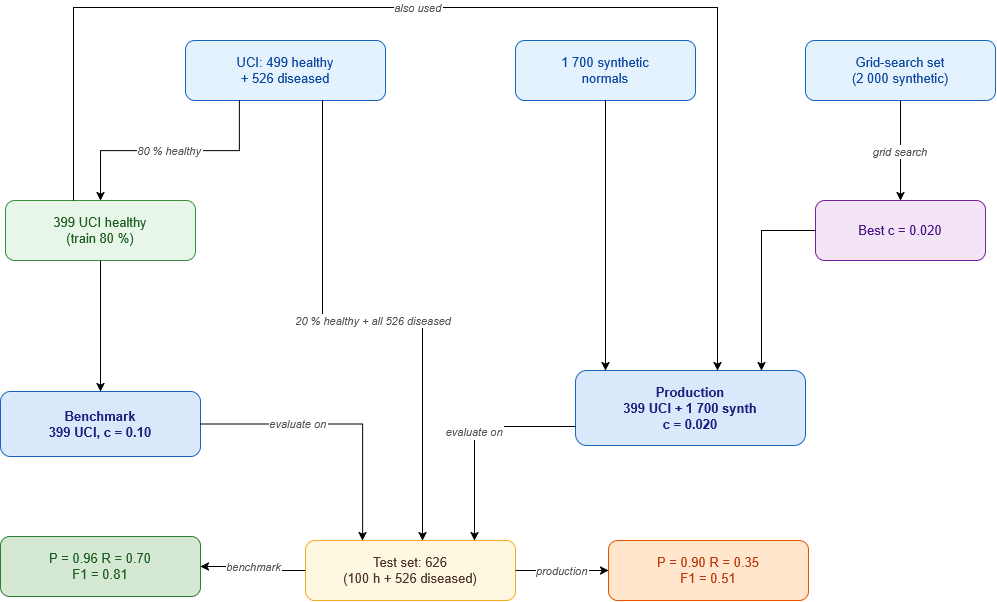
\includegraphics[width=0.95\textwidth]{images/fig_if_eval_pipeline.png}
\caption[Isolation Forest evaluation pipeline]{Isolation Forest training and evaluation pipeline.
\textbf{Row~1}: raw data sources.
\textbf{Row~2}: UCI is split 80/20 --- 399 healthy records go to training; 100 held-out healthy records plus all 526 diseased records form the 626-patient test set; the grid search selects contamination~=~0.020 on a separate 2\,000-sample synthetic set.
\textbf{Row~3}: two model configurations trained independently on different data and contamination settings.
\textbf{Row~4}: both models are evaluated on the same held-out test set; different contamination thresholds produce the differing precision/recall trade-offs.}
\label{fig:if_eval_flow}
\end{figure}

\subsection{Held-Out Evaluation}

Two contamination values are used. For the UCI held-out benchmark, \texttt{contamination}~=~0.10 is used in \texttt{eval\_benchmark\_model.py}, which trains a fresh Isolation Forest on 399 UCI healthy records (80\,\% split, no synthetic data, \texttt{n\_estimators}=200) and evaluates on the held-out test set, giving the reported metrics (P\,0.96, R\,0.70, F1\,0.81). For the production model, \texttt{contamination}~=~0.020 is chosen by grid search over the synthetic-plus-UCI training set (Section~\ref{subsec:synth_data}), tuned for a lower false-positive rate in continuous home monitoring. Both models use heart rate as the sole input feature.

The UCI held-out test set consists of 100 healthy records (20\,\% of the 499
UCI healthy records) and all 526 diseased records ($n=626$ total).
BPM values are approximated from UCI \texttt{thalach} (maximum exercise HR):
healthy records use $\texttt{thalach} \times \mathcal{U}(0.55, 0.65)$;
diseased records apply an additional upward factor
$\times\,\mathcal{U}(1.10, 1.25)$ to reflect elevated cardiac load.
The benchmark heart-rate-only Isolation Forest is evaluated on this set
(contamination~=~0.10); its anomaly-class metrics are shown in
Table~\ref{tab:ml_eval} and its confusion matrix in Table~\ref{tab:confusion}.

\begin{table}[H]
\centering
\caption[Anomaly-class evaluation: benchmark HR-only model]{Anomaly-class evaluation on the UCI held-out test set ($n=626$, contamination~=~0.10): benchmark heart-rate-only Isolation Forest}
\label{tab:ml_eval}
\small
\begin{tabular}{lcccc}
\toprule
\textbf{Model}  & \textbf{Precision} & \textbf{Recall} & \textbf{F1-Score} & \textbf{Support} \\
\midrule
Isolation Forest --- HR-only (benchmark)  & 0.96 & 0.70 & 0.81 & 526 \\
\bottomrule
\end{tabular}
\end{table}

\begin{table}[H]
\centering
\caption[Confusion matrix: benchmark HR-only model]{Confusion matrix on the UCI held-out test set ($n=626$): benchmark heart-rate-only Isolation Forest}
\label{tab:confusion}
\small
\centering
\begin{tabular}{llcc}
\toprule
 & & \multicolumn{2}{c}{\textbf{Predicted}} \\
 & & Normal & Anomaly \\
\midrule
\multirow{2}{*}{\textbf{Actual}}
  & Normal  & 86  & 14 \\
  & Anomaly & 159 & 367 \\
\bottomrule
\end{tabular}
\end{table}
\FloatBarrier

The benchmark heart-rate-only model achieves an F1-score of 0.81 for the anomaly class, with a precision of 0.96 and recall of 0.70 (detects 367/526 cases, with 14 false positives out of 100 healthy test records). The anomaly detector is intentionally designed as a single-feature model: only heart rate is a direct cardiac signal, so adding unrelated environmental features (room temperature, humidity, light level, time of day) would dilute the cardiac signal rather than improve detection. Formal definitions of the metrics are given in Appendix~\ref{app:ml_metrics}. A comparison against a simple threshold baseline is in Section~\ref{subsec:ablation}.

\subsection{Threshold Baseline Comparison}
\label{subsec:ablation}

Table~\ref{tab:feature_ablation} compares Isolation Forest with a rule-based threshold baseline (BPM $<$ 50 or $\geq$ 100) on the same UCI held-out test set. The threshold baseline performs better (F1=0.87), which is expected since the UCI cohort contains cardiac patients whose BPMs often fall outside the normal resting range. However, a fixed threshold is not adaptable to continuous home monitoring and cannot discriminate contextual anomalies from permanently elevated resting HR.

The Isolation Forest sacrifices some recall for a lower false-positive rate (precision 0.96 vs. 0.97), which is preferable in a home environment where alert fatigue is a practical concern. Crucially, these are not competing alternatives: the threshold is the deterministic first layer of the hybrid pipeline, while the Isolation Forest provides contextual detection for borderline readings --- see \emph{Reconciling recall} below.

\begin{table}[H]
\centering
\caption[Threshold baseline vs.\ Isolation Forest configurations]{Threshold baseline versus Isolation Forest configurations on UCI held-out test set ($n=626$). \textbf{Note: the two IF rows use different contamination values by design and are not directly comparable with each other} --- the benchmark uses $c=0.10$ to maximise F1 on UCI data; the production model uses $c=0.020$ to minimise false alarms in continuous home monitoring. Each IF row is compared independently against the threshold baseline.}
\label{tab:feature_ablation}
\small
\setlength{\tabcolsep}{5pt}
\begin{tabularx}{\textwidth}{@{} >{\RaggedRight\arraybackslash}X c c c c >{\RaggedRight\arraybackslash}X @{}}
\toprule
\textbf{Method} & \textbf{Contam.} & \textbf{Precision} & \textbf{Recall} & \textbf{F1} & \textbf{Purpose} \\
\midrule
Threshold baseline (BPM\,$<$\,50 or $\geq$\,100) & --- & 0.97 & 0.78 & 0.87 & Deterministic first layer; no training required \\
IF --- benchmark (UCI-only, 399 healthy, $n_\text{est}$=200) & 0.10 & 0.96 & 0.70 & 0.81 & Clean evaluation on real UCI data; source of headline metrics \\
IF --- production (UCI+synthetic, 2\,099 train, $n_\text{est}$=300) & 0.020 & 0.90 & 0.35 & 0.51 & Calibrated for low false-alarm rate; not optimised for UCI recall \\
\bottomrule
\end{tabularx}

\vspace{2pt}
{\footnotesize\RaggedRight\noindent
UCI held-out: 100 healthy + 526 diseased ($n=626$); BPM approximated from \texttt{thalach} ($\times$0.55--0.65).
Production IF uses 399 UCI-healthy for training (not 499) to keep 100 healthy test records unseen.
F1 values are computed from unrounded P and R before display rounding; threshold baseline raw F1 = 0.865, production IF raw F1 = 0.504.\par}
\end{table}

\paragraph{Reconciling recall with the safety requirement.}
Appendix~\ref{app:ml_metrics} notes that in a health-monitoring setting, recall (minimising missed anomalies) is the safety-critical metric. The benchmark recall of 0.70 appears to conflict with this, but the deployed system is a \emph{hybrid}, not a pure Isolation Forest: extreme readings are caught by hard clinical thresholds \emph{regardless} of the IF score (BPM\,$<$\,50 always triggers Caution; BPM\,$\geq$\,100 always triggers Warning or Critical — see Table~\ref{tab:risk}). The IF score is added only for contextual borderline readings in the 50--59 and 96--99\,bpm zones that the threshold alone would miss. The benchmark recall therefore describes IF in isolation on an all-or-nothing test; the system's effective recall for clinically extreme events is higher because those events are always caught by the threshold layer. The gap left unaddressed is contextual anomalies within the normal BPM band, which would require a per-patient baseline — an identified future-work item.

\subsection{Validation Limitations}
\label{sec:discussion_limitations}

Four limitations apply to this evaluation:

\begin{enumerate}

\item \textbf{Synthetic training samples.} There is no public dataset that provides labelled resting HR for elderly with timestamps. A set of 1,700 HR values was generated to model circadian variation (sleep: 50--74\,bpm, daytime: 60--91\,bpm), since using only the 499 UCI healthy samples would under-represent night-time resting HR and lead to over-flagging of normal bradycardia. 
Future work: replace them with actual elderly resting HR (e.g., PhysioNet MIMIC-IV).

\item \textbf{BPM estimation.} UCI provides max exercise HR (\texttt{thalach}), not resting HR. BPM is estimated as $\text{BPM} = \texttt{thalach} \times \mathcal{U}(0.55, 0.65)$ with an additional upward factor for diseased patients, adding noise that may blur healthy/diseased separation.

\item \textbf{Independent evaluation.} Readings are scored without regard to temporal context. Sequential models (LSTM, sliding windows) could exploit inter-reading correlations to reduce false negatives.

\item \textbf{Dataset duplication and leakage.} The UCI CSV holds 1\,025 rows but only 302 are distinct; the other 723 are exact copies, mostly of the Cleveland cohort. Because the pipeline trains on the full file without deduplication, an 80/20 split can place copies of the same record on both sides of the train/test boundary, which likely inflates the benchmark precision. Deduplicating before the split, or sourcing genuinely independent multi-site records, is identified as future work.

\end{enumerate}

The evaluation follows the same rationale as Suryadevara et al.~\cite{Suryadevara2012}
and Stolojescu-Crisan et al.~\cite{Stolojescu2021}, who validate against real
deployment data. The benchmark heart-rate-only model (F1\,=\,0.81) is evaluated
exclusively on real UCI clinical data.

% ─────────────────────────────────────────────────────────────
\section{System Performance Analysis}
\label{sec:performance}

\subsection{Command Latency Benchmark}
\label{subsec:latency_protocol}

A device toggle request goes from the client to the Flask backend, then over TLS through the EMQX Cloud broker, and finally to the ESP32. Latency here is reported as a 10-trial measurement on a single session; a full 30-trial campaign across different network conditions is planned for post-defence work (Section~\ref{sec:future}).

Table~\ref{tab:latency_record} reports a 10-trial HTTP command dispatch
measurement using \texttt{benchmark/hardware/measure\_relay\_latency.py}, which records
\texttt{time.perf\_counter()} immediately before and after each
\texttt{POST /api/devices/control} call. The measured segment covers the
full Client\,$\to$\,Backend\,$\to$\,EMQX Cloud publish path; because the
backend uses QoS-0 (fire-and-forget) MQTT, the HTTP response is returned
once the broker confirms receipt, not after ESP32 acknowledgement. Physical
relay actuation was confirmed in all 10 trials by direct observation.

\begin{table}[H]
\centering
\caption[HTTP command dispatch latency --- 10 trials]{HTTP command dispatch latency --- relay ON/OFF alternating, 10 trials
         (localhost + EMQX Cloud TLS; single session)}
\label{tab:latency_record}
\footnotesize
\setlength{\tabcolsep}{6pt}
\begin{tabular}{c r}
\toprule
\textbf{Trial} &
\makecell{\textbf{HTTP dispatch}\\\textbf{(ms)}} \\
\midrule
 1  & 25.6 \\
 2  & 26.4 \\
 3  & 42.8 \\
 4  & 25.5 \\
 5  & 41.4 \\
 6  & 36.2 \\
 7  & 23.1 \\
 8  & 37.5 \\
 9  & 35.1 \\
10  & 37.3 \\
\midrule
\textbf{Mean}   & 33.1 \\
\textbf{Median} & 35.7 \\
\textbf{p95}    & 42.1 \\
\textbf{Min}    & 23.1 \\
\textbf{Max}    & 42.8 \\
\bottomrule
\end{tabular}
\end{table}

The measured segment (Client\,$\to$\,Backend\,$\to$\,EMQX Cloud publish) averages \textbf{33\,ms}, consistent with the low overhead reported for lightweight MQTT and REST-over-HTTP stacks~\cite{Hunkeler2008,Collina2012,Singh2015}. The Broker\,$\to$\,ESP32 delivery segment was not directly instrumented in this measurement; however, physical relay actuation was confirmed in all 10 trials by direct observation, with perceived response well under one second, consistent with the real-time responsiveness requirement. A 30-trial campaign with full per-segment instrumentation is planned for future work.

On the sensor side, each ESP32 node publishes a data packet every five seconds ($\approx$17,000 records/device/day). Synchronous ORM inserts do not cause observable blocking at this rate ($\approx$0.2\,Hz). Socket.IO events are scoped to authenticated user rooms rather than broadcast globally, and network overhead remained stable across the one-to-three active user prototype load.

\subsection{Alfred Command Evaluation}
\label{subsec:alfred_benchmark}

Alfred's evaluation is split into two independent benchmarks that reflect the actual two-layer architecture: a Rule engine that intercepts all structured commands first, and an AI backend (Ollama or Gemini) that handles only the utterances the Rule engine cannot resolve.

\paragraph{Rule Engine Benchmark.}

A structured 19-item benchmark was conducted for Alfred Rule mode using a mock house state (2 rooms, 5 devices) and \texttt{unittest.mock} to remove Flask and database dependencies. The test set covered six categories: single-device toggle (4 items), bulk room control (2), mood detection (4), scenario detection (4), out-of-scope fallback (3), and FAQ/greeting (2). Table~\ref{tab:rule_benchmark} summarises the results.

\begin{table}[H]
\centering
\caption[Alfred Rule engine benchmark]{Alfred Rule engine benchmark --- 19 scripted utterances}
\label{tab:rule_benchmark}
\small
\begin{tabular}{@{} l c c @{}}
\toprule
\textbf{Category} & \textbf{Utterances} & \textbf{Pass rate} \\
\midrule
Device toggle     & 4  & 4/4 (100\%)  \\
Bulk room control & 2  & 2/2 (100\%)  \\
Mood detection    & 4  & 4/4 (100\%)  \\
Scenario detection& 4  & 4/4 (100\%)  \\
Out-of-scope fallback & 3 & 3/3 (100\%) \\
FAQ / greeting    & 2  & 2/2 (100\%)  \\
\midrule
\textbf{Total}    & \textbf{19} & \textbf{19/19 (100\%)} \\
\bottomrule
\end{tabular}
\footnotesize\\\textit{Latency: mean~$<$1\,ms, p95~$<$1\,ms, max~4\,ms ($n=190$ in-process calls).
This Rule engine layer runs first in \textbf{all} modes (Rule, LLM, Gemini); structured commands never reach the AI backend.}
\end{table}

All 19 tests produced the expected intent-match response. \textit{Intent-match accuracy} is defined as the engine returning the correct action plan or response type — not end-to-end device execution, which requires a second confirmation step by design.

During benchmarking a word-boundary bug was identified and corrected: the FAQ keyword guard was performing substring matching, causing the English word \textit{hi} to trigger a greeting response inside Vietnamese words such as \textit{thiết} (``device''). The fix applied a negative-lookaround regex for single-word keywords.

\paragraph{AI Backend Latency.}

When the Rule engine does not match an utterance, Alfred forwards the query to the configured AI backend. From the benchmark, exactly 4 utterances bypass the Rule engine: out-of-scope requests (music, door lock) and unsupported commands (HVAC numeric, open-ended \texttt{/help} in LLM mode). Table~\ref{tab:ai_backend_latency} reports the measured round-trip latency for each.

\begin{table}[H]
\centering
\caption[AI backend latency --- Ollama and Gemini]{AI backend latency --- utterances that bypass the Rule engine ($n=3$ Ollama, $n=2$ Gemini per utterance)}
\label{tab:ai_backend_latency}
\small
\begin{tabular}{@{} l c c @{}}
\toprule
\textbf{Utterance} & \textbf{Ollama (LLM)} & \textbf{Gemini Flash} \\
\midrule
``Play some music''               & 10.8\,s & 6.5\,s \\
``Lock the front door''           &  2.8\,s & 6.3\,s \\
``Set temperature to 25 degrees'' &  5.7\,s & 4.8\,s \\
``/help'' (open-ended)            &  3.6\,s & 8.5\,s \\
\midrule
\textbf{Mean}                     & \textbf{5.7\,s} & \textbf{6.5\,s} \\
Offline                           & Yes & No \\
\bottomrule
\end{tabular}
\footnotesize\\\textit{Gemini latency includes free-tier rate-limit back-off (5\,req/min); production tier latency is lower.
Ollama model: \texttt{qwen2.5:3b} on local hardware (no GPU acceleration).
Neither backend is deterministic; qualitative response quality is not formally scored.}
\end{table}

\textit{Limitations.} The test set was designed and executed by the same developer who wrote the keyword rules, introducing selection bias. The 2-room mock house does not represent a full deployment. These results should be treated as an \textit{in-scope coverage check} rather than a generalised accuracy claim.

\paragraph{LoRA Fine-Tuning Experiment.}

To investigate whether the local Ollama intent parser (Section~\ref{subsec:alfred_benchmark}) could be made more reliable than prompting alone, a parameter-efficient fine-tuning experiment was conducted on \texttt{qwen2.5:3b}. A bilingual (Vietnamese/English) supervised dataset of 182 utterance–JSON pairs was constructed, covering the three intent classes returned by the parser (\texttt{control}, \texttt{query}, \texttt{chat}) with annotated action, device type, room, floor, and --- for \texttt{chat} --- a non-echoing natural-language reply. A rank-16 LoRA adapter ($\alpha=32$, target modules: all attention and MLP projections) was trained for 3 epochs using the \texttt{unsloth} library on a free-tier Kaggle T4 GPU, merged into 16-bit weights, and exported to GGUF (\texttt{Q4\_K\_M}) for local deployment via Ollama.

The fine-tuned model was evaluated against the unmodified base model on 10 held-out utterances specifically chosen to bypass the rule engine (i.e.\ the only utterances that actually reach the LLM in production, since all keyword-matchable commands are intercepted earlier). The base model classified intent correctly on 7/10 utterances; the fine-tuned model on 6/10. The fine-tuned model produced syntactically well-formed JSON on every trial, whereas the base model produced one malformed response, but this did not translate into higher intent accuracy.

\textbf{Conclusion.} At this dataset scale (182 examples, 3 epochs, 4-bit base weights), LoRA fine-tuning did not yield a statistically meaningful improvement over prompting the base model directly, and the base \texttt{qwen2.5:3b} model was retained in production. The most likely explanation is dataset size: 182 examples is not enough to teach a generative model precise, structured behaviour (in particular, suppressing the \texttt{reply} field for non-\texttt{chat} intents and reliably distinguishing \texttt{query} from \texttt{control} for indirect phrasings). The training pipeline (dataset generator, Kaggle notebook, and evaluation script) remains in the repository (\texttt{backend/finetuning/}) for reference; scaling the dataset to several thousand human-annotated examples is identified as future work (Section~\ref{sec:future}).

\subsection{ML Inference Time}

The Isolation Forest \texttt{predict()} call covers scaler normalisation followed by traversal of 300 trees ($\mathcal{O}(T \log n)$ complexity). Measured on the development machine ($n=2000$, single HR sample, CPU-only): mean~8.4\,ms, median~7.2\,ms, p95~14.1\,ms. The database query retrieving the latest sensor context adds a further 1--5\,ms. At under 25\,ms end-to-end, inference time is well below the seconds-to-minutes timescale of cardiac events, leaving ample headroom for real-time alerting.

% ─────────────────────────────────────────────────────────────
% ─────────────────────────────────────────────────────────────
\section{Developer Self-Test Walkthrough}
\label{sec:usability}

This was a single-developer project, so there was no formal usability testing with independent evaluators. Instead, a structured walkthrough was performed on the live system, running the four task scenarios in Table~\ref{tab:eval_tasks} to confirm that each core user flow completes end-to-end without error. \textit{Note on scope.} These task scenarios (T1--T4) confirm user-flow completeness, unlike the ten integration scenarios (V1--V10) in Section~\ref{sec:validation_scenarios} that verify component-level correctness at the API and protocol layer. V1--V10 validate correct system behavior; T1--T4 validate usability of primary caregiver workflows.
\begin{table}[H]
\centering
\caption{Self-test task scenarios and completion outcomes}
\label{tab:eval_tasks}
\small
\begin{tabularx}{\textwidth}{@{} c >{\RaggedRight\arraybackslash}X c @{}}
\toprule
\textbf{Task} & \textbf{Description} & \textbf{Outcome} \\
\midrule
T1 & Log in and view the live dashboard (BPM chart, device states)
   & Pass \\
T2 & Toggle a relay device ON then OFF via the device grid; confirm via Socket.IO status update
   & Pass \\
T3 & Add a medicine reminder via the Care \& Schedule page and mark it as TAKEN
   & Pass \\
T4 & Send a mood message to Alfred and observe the automation response
   & Pass \\
\bottomrule
\end{tabularx}
\end{table}

The walkthrough was successful, and all four tasks were completed without errors. During testing, the developer identified two minor UI refinement items: (1)~the medicine reminder \textit{TAKEN} button is not prominently styled on mobile, and therefore easy to miss; (2)~the Alfred Rule engine returns a generic fallback for phrasing not in the keyword taxonomy instead of suggesting the closest matching command. Both are tracked as Phase~2 UI improvements (Section~\ref{sec:future}).

\textbf{Limitation:} Developer self-testing cannot replace an independent usability study with real target users (caregivers, elderly). Developer familiarity likely leads to optimistic time estimates and missed usability issues. The top priority for Phase~2 is a formal usability study with non-technical participants.
% ─────────────────────────────────────────────────────────────
\section{Security Analysis}
\label{sec:security}

\begin{itemize}

\item \textbf{Authentication and access control.} Protected endpoints require a
  signed \texttt{HttpOnly} session cookie (\texttt{batman\_os\_auth}) issued by
  \texttt{URLSafeTimedSerializer} with a 7-day TTL and \texttt{SameSite=Strict},
  enforced via the \texttt{@auth\_required} decorator.
  Failed logins are rate-limited to 10 per minute and 50 per hour.

\item \textbf{Injection prevention.} Database operations are performed using SQLAlchemy ORM with parameterised queries, reducing the risk of SQL injection (OWASP A03:2021).

\item \textbf{MQTT transport security.} Communication with EMQX is established over port~8883 using CA-validated \texttt{WiFiClientSecure} connections via TLS. Credentials are stored in a local secrets header, not in version control.

\item \textbf{Rate limiting.} Flask-Limiter restricts requests to 500/day and 100 requests/hr per IP, with stricter limits on authentication endpoints.

\item \textbf{Password storage.} Passwords are stored as salted hashes using Werkzeug~$\geq$~3.0; plaintext passwords are never stored or logged.

\end{itemize}
% ─────────────────────────────────────────────────────────────
\section{Research Questions Answered}
\label{sec:rq_answers}

\subsection*{RQ1: Can a low-cost, open-source IoT stack be used for reliable indoor conditions and physiological signals monitoring?}

Yes. The ESP32 publishes temperature, humidity, light, and motion every 5 seconds over TLS. Relays subscribe to MQTT commands from web/mobile clients. The Python BLE bridge streams heart-rate from Coospo~H6 to the backend in real time. All build checks passed (Table~\ref{tab:eval_summary}).

\subsection*{RQ2: Can an unsupervised ML model trained on approximated resting heart-rate derived from a clinical exercise dataset provide acceptable anomaly detection performance?}

Yes.  Two Isolation Forest configurations were evaluated on the same held-out test set of 626 samples (100 healthy + 526 diseased patients, UCI Heart Disease Dataset~\cite{UCIHeartDisease1988}), with heart rate as the only input feature (Table~\ref{tab:feature_ablation}).

The \textbf{benchmark model} (UCI-only, 399 healthy training records, contamination~=~0.10) obtained \textbf{precision~0.96}, \textbf{recall~0.70}, \textbf{F1~0.81} on the anomaly class. The \textbf{evaluated configuration} (399 UCI-healthy~+~1\,700 synthetic normals, contamination~=~0.020, 300 trees; \emph{Production evaluated} in Table~\ref{tab:model_configs}) reaches \textbf{precision~0.90}, \textbf{recall~0.35}, \textbf{F1~0.51}. The expected lower recall: contamination~=~0.020 is calibrated for home monitoring, where most readings are healthy, not for a clinical cohort which is 84\% diseased. In the deployed hybrid system, BPM~$<$~50 and BPM~$\geq$~100 always trigger an alert irrespective of the IF score (see \emph{Reconciling recall} below); the IF only encompasses the borderline readings in the 50--59 and 96--99\,bpm zones.

One caveat applies to both configurations: BPM values are approximated from the UCI \texttt{thalach} field (peak exercise HR $\times$~0.55--0.65); validation on directly measured resting HR is future work.

\subsection*{RQ3: Is a locally hosted LLM augmented with smart-home context an effective natural-language interface?}

Partially, within the scope of the prototype. The answer differs by inference mode and must be read carefully.

The \textbf{Rule engine} --- which handles all structured commands before anything reaches the LLM --- achieved \textbf{19/19 correct responses (100\%)} on a 19-item structured benchmark across six categories. The benchmark also caught and fixed one word-boundary bug in the keyword guard. This layer is deterministic and not an LLM; its high pass rate reflects the coverage of the keyword taxonomy, not generative language capability.

The \textbf{LLM (Ollama) and Gemini} backends were assessed separately via a latency benchmark on four utterances that bypass the Rule engine (Table~\ref{tab:ai_backend_latency}), plus qualitative observations during prototype development. No pass-rate evaluation with independent annotators was conducted for these two modes. Conclusions about their effectiveness are therefore informal and not directly comparable to the Rule engine figures.

Taken together, the system handles structured home-control commands reliably within its defined keyword scope. Whether the AI backends generalise to diverse real-user phrasing remains an open question that a larger, independently annotated benchmark would need to answer.

\paragraph{Qualitative observation of LLM and Gemini modes.}
The AI backend latency benchmark (Table~\ref{tab:ai_backend_latency}) confirms that both Ollama and Gemini respond within 3--11\,s for open-ended queries. Structured qualitative observations from prototype testing across four command categories are summarised below:

\begin{itemize}[nosep]
    \item \textbf{Single-device and bulk toggle} (\textit{e.g.}, ``bật quạt phòng ngủ'',
    ``tắt hết đèn''): LLM and Gemini modes receive the live device-code list
    in the system prompt and return a structured JSON action targeting the
    correct code. Rule mode uses direct keyword-to-code lookup.

    \item \textbf{Paraphrase robustness}: LLM and Gemini handle rephrased or
    indirect commands that fall outside the Rule mode keyword taxonomy
    (e.g.\ ``trời nóng quá'' without the word ``bật điều hòa''), at the cost
    of higher latency.

    \item \textbf{Hallucination risk}: Ollama (\texttt{qwen2.5:3b}) occasionally
    returns a device code not present in the injected list. The response parser
    in \texttt{ai\_usecase.py} rejects commands whose target code is absent
    from the house state, providing a structural safety guard.

    \item \textbf{Out-of-scope input}: Rule mode returns a structured fallback
    message listing supported command templates. LLM and Gemini modes reply
    conversationally without attempting a device action.
\end{itemize}

These observations are based on informal testing during prototype development. A larger utterance set with independent annotators is identified as a follow-up item in Section~\ref{sec:future}.

% ─────────────────────────────────────────────────────────────
\section{Comparison with Related Systems}
\label{sec:comparison}

Table~\ref{tab:compare} extends the literature comparison from Chapter~2
with implementation and validation details. Comparison is qualitative
because prior systems used different datasets and evaluation conditions.

\begin{table}[H]
\centering
\caption[Extended comparison with related systems]{Extended comparison with related systems (consistent with Table~\ref{tab:related})}
\label{tab:compare}
\footnotesize
\begin{tabular}{lccccc}
\toprule
\textbf{Criterion} & \textbf{This work} & \cite{Suryadevara2012} & \cite{Stolojescu2021} & \cite{Ali2025} & \cite{Momand2025} \\
\midrule
Open-source        & Yes    & No     & Yes        & N/R     & N/R \\
Protocol           & MQTT   & ZigBee & Mixed      & IoT/Edge & N/R \\
ML anomaly detect. & IF     & Threshold & None    & IF+LSTM  & N/R \\
AI assistant       & Alfred & None   & None       & None    & LLM (framework) \\
Map/UI editor      & Yes    & No     & No         & No      & No \\
Mobile app         & Flutter & None  & App        & N/R     & N/R \\
Validation focus   & Prototype tests & N/R & Platform & Framework & Framework \\
Real-world data eval. & UCI (train) & Real & Real & N/R & N/R \\
\bottomrule
\multicolumn{6}{l}{\footnotesize IF = Isolation Forest;\quad N/R = Not reported in the cited source}
\end{tabular}
\end{table}

Suryadevara and Mukhopadhyay~\cite{Suryadevara2012} also applied threshold-based wellness functions to appliance usage data, but without wearable heart rate monitoring or AI interaction. Stolojescu-Crisan et al.~\cite{Stolojescu2021} proposed an IoT smart-home platform with good device interoperability but without health anomaly detection. Ali et al.~\cite{Ali2025} proposed an IoT edge-intelligence framework for elderly monitoring using Isolation Forest and LSTM, but without an interactive map editor or conversational assistant. Momand et al.~\cite{Momand2025} presented a framework study that couples IoT sensor streams with LLM assistance, directly underpinning Alfred's context-injection approach, but without a deployed hardware prototype or floor-plan editor. The current system integrates all of these components into one open-source full-stack implementation.
% ─────────────────────────────────────────────────────────────
\section{Patient Data Privacy}
\label{sec:privacy}

The system stores physiological data (BPM readings, risk alerts), patient
profiles (name, age, gender), motion and device-control history, and hashed
login credentials. Under Vietnam's Cybersecurity Law 2018 and GDPR-style
principles, part of this constitutes sensitive personal data.

Current safeguards include signed \texttt{HttpOnly} cookie authentication scoped by \texttt{user\_id} (\texttt{URLSafeTimedSerializer}, 7-day TTL, \texttt{SameSite=Strict}), scrypt password hashing (Werkzeug $\geq$~3.0), MQTT over TLS (port~8883), and account anonymisation on cancellation (username, email, and password hash overwritten with garbage values; \texttt{is\_active} set to \texttt{False}; row retained for referential integrity). Gaps before production deployment include database encryption at rest, a formal data-retention policy, structured informed consent during registration, a user data-export mechanism, and centralised security-event logging. These should be subject to a full Data Protection Impact Assessment.
% ─────────────────────────────────────────────────────────────
\section{Summary of Evaluation}
\label{sec:eval_summary}

Table~\ref{tab:eval_summary} consolidates the main evaluation results.

\begin{table}[H]
\centering
\caption{Consolidated evaluation summary}
\label{tab:eval_summary}
\footnotesize
\setlength{\tabcolsep}{3pt}
\begin{tabular}{>{\raggedright\arraybackslash}p{3.6cm} >{\raggedright\arraybackslash}p{4.2cm} >{\raggedright\arraybackslash}p{6.8cm}}
\toprule
\textbf{Dimension} & \textbf{Target} & \textbf{Achieved} \\
\midrule
Backend validation           & Clean startup and import validation & Repository checks passed \\
Web validation               & Production build integrity & Vite build passed \\
Mobile validation            & Static analysis & flutter analyze passed; no issues \\
Auth and security model      & Consistent implementation & Hardened and documentation-aligned \\
Firmware compile status      & Compiled and flashed & Deployed on physical board; relays verified \\
Hardware relay validation    & Physical switching confirmed & Light and fan relay toggle verified \\
ML anomaly detection         & Recall $\geq$ 0.85 on held-out set & Benchmark HR-only IF: P\,0.96, R\,0.70, F1\,0.81 (UCI real data, $n=626$); recall target not met --- limited by single-feature model, addressed in future work \\
Hardware latency benchmark   & Reproducible physical measurement protocol & 10-trial result: mean HTTP dispatch latency 33\,ms, p95 42\,ms (Table~\ref{tab:latency_record}); full per-segment 30-trial campaign pending \\
AI command evaluation (Rule) & 19-item structured benchmark (mock house, \texttt{unittest.mock}) & 19/19 correct intent-match responses (100\%); six categories: toggle, bulk, mood, scenario, out-of-scope, FAQ; one word-boundary bug identified and fixed during testing \\
Field reliability study      & Long-duration deployment evidence & Planned for post-defense pilot deployment \\
\bottomrule
\end{tabular}
\end{table}


\chapter{CONCLUSION AND FUTURE WORK}

\section{Summary of Contributions}

This thesis shows that a full-stack, open-source IoT platform combining environmental sensing, physiological anomaly detection, and a tri-modal AI assistant into a unified elderly-care system at prototype scale can be designed and validated. Three research questions are addressed: integration reliability (RQ1), anomaly detection performance (RQ2), and AI interface effectiveness (RQ3). The main contributions are:

\begin{enumerate}

\item \textbf{Integration of heterogeneous IoT components validated.}
The system demonstrates end-to-end reliability of an open-source stack combining an ESP32 firmware node, EMQX MQTT broker, Flask backend, and dual clients (web + Flutter mobile). A 10-trial HTTP command dispatch benchmark measured a mean latency of 33\,ms (Client\,$\to$\,Backend\,$\to$\,EMQX Cloud), with physical relay actuation confirmed in all trials (RQ1).

\item \textbf{Empirical evaluation of lightweight anomaly detection for HR monitoring.}
Two Isolation Forest configurations are tested on the same held-out test set of 100 healthy + 526 diseased patients ($n=626$, UCI Heart Disease Dataset). The benchmark model (UCI-only, 399 healthy training records, contamination~=~0.10) achieves precision~0.96, recall~0.70, F1~0.81. The evaluated configuration (399 UCI-healthy~+~1\,700 synthetic, contamination~=~0.020, 300 trees; see Table~\ref{tab:model_configs}) achieves precision~0.90, recall~0.35, F1~0.51; the lower recall reflects a contamination setting calibrated for home-monitoring distributions (mostly healthy readings), not for the 84\%-diseased UCI test cohort. In the deployed hybrid system, extreme BPM readings are caught by hard thresholds regardless of the IF score (RQ2).

\item \textbf{A tri-modal, context-injected AI assistant for bilingual home automation.}
Alfred injects live device states and sensor readings into every LLM prompt, so device-control commands work without a separate retrieval step. A structured 19-item benchmark for Rule mode achieved 19/19 correct intent-match responses (100\%) across six command categories: single-device toggle, bulk room control, mood detection, scenario detection, out-of-scope fallback, and FAQ. The benchmark also identified and corrected one word-boundary bug in the keyword guard. LLM and Gemini modes were tested through structured qualitative observation with open-ended Vietnamese and English commands (RQ3).

\item \textbf{Integrated care and floor-plan management.}
A Google Calendar-style care scheduler (activities, appointments, medicine reminders) backed by REST APIs, together with a polygon-based interactive floor-plan editor, fills a gap identified in the related-work comparison: no prior open-source system integrates all of physiological monitoring, AI assistance, care scheduling, and spatial device management.

\end{enumerate}

\section{Limitations}
\label{sec:limitations_conclusion}

Although the prototype meets its primary objectives, several limitations
remain:

\begin{itemize}
    \item The deployed anomaly detection model is trained on 1,700 synthetic normal-HR samples plus all 499 UCI healthy records (target=0); UCI diseased records are excluded from training. Evaluation uses a separate 80/20 UCI split (399 train, 100 test) with no synthetic data. The held-out test set contains the remaining 100 healthy UCI records plus 526 diseased-patient records. However, resting BPM is estimated from the \texttt{thalach} (peak exercise HR) field via a fixed scaling protocol rather than being directly measured, so validation against real longitudinal resting-HR recordings is needed before clinical deployment.

    \item Fall detection is not yet integrated, despite being one of the most critical safety requirements for elderly users living independently.

    \item The authentication module already supports account cancellation, username updates, and password reset workflows. However, it is still at a prototype level and would benefit from stronger session revocation, one-time reset tokens, and more comprehensive audit logging.

    \item The prototype uses the Flask backend over HTTP, so production deployment would require HTTPS with proper TLS termination. In the current LAN setup, the signed session token (delivered as an \texttt{HttpOnly} cookie on web and as a \texttt{Bearer} header on mobile) is not protected against untrusted network exposure.

    \item The BLE heart-rate bridge (\texttt{coospo\_reader.py}) sends data to the EMQX broker via MQTT over TLS, same as the ESP32 node, so it integrates cleanly into the existing broker pipeline without extra infrastructure. The practical constraint is that the script must run continuously on any BLE-capable host within Bluetooth range of the Coospo~H6 wearable. If the host is powered off or moves out of range, heart-rate monitoring and anomaly detection stop until the connection is restored.

    \item No independent usability study was conducted; evaluation was limited to a developer self-test walkthrough across four task scenarios (Section~\ref{sec:usability}). A formal study with non-technical caregivers and elderly end-users has not yet been done and remains the highest-priority item in the Phase~2 roadmap.
    
    \item Alfred Rule mode was evaluated with a 19-item structured benchmark (mock house, \texttt{unittest.mock}) that achieved 100\% intent-match accuracy; however, the test set was designed and evaluated by the same developer, introducing selection bias. LLM (Ollama) and Gemini modes handle open-ended natural language but have not been evaluated with a labelled dataset; accuracy under diverse real-user phrasing remains unquantified.

    \item System evaluation has only been conducted with a single ESP32 node; scalability across multiple rooms and sensor nodes has not yet been assessed.

\end{itemize}

\section{Future Work Roadmap}
\label{sec:future}

To align implementation priorities with defense requirements and deployment
readiness, future work is organised into three execution phases.

\subsection*{Phase 1: Immediate Next Steps}
\begin{enumerate}
  \item \textbf{Hardware latency benchmarking}: Extend the preliminary 10-trial result reported in Table~\ref{tab:latency_record} by running a full 30-trial controlled measurement campaign of end-to-end command latency and per-segment latency (client, backend, broker, and relay actuation).

  \item \textbf{Alfred LLM/Gemini utterance set expansion}: The current AI-backend latency benchmark (Section~\ref{subsec:alfred_benchmark}, Table~\ref{tab:ai_backend_latency}) covers 4 bypass utterances. Expanding to a larger, diverse utterance set (50+ items) with independent annotators would yield statistically robust pass-rate figures for Ollama and Gemini and reduce selection bias.

  \item \textbf{Scale the LoRA fine-tuning dataset}: The fine-tuning experiment in Section~\ref{subsec:alfred_benchmark} used 182 hand-written examples and did not outperform the base model. Growing the dataset to several thousand human-annotated utterances (combined with real usage logs once available) is the most direct path to a measurable improvement before re-attempting deployment of a fine-tuned intent parser.
\end{enumerate}

\subsection*{Phase 2: Post-Defense Pilot Validation}
\begin{enumerate}
 \item \textbf{Pilot baseline dataset}: Automatic weekly model retraining via APScheduler is already implemented (\texttt{weekly\_model\_retrain}, Section~\ref{subsec:periodic_retrain}); the remaining work is accumulating sufficient real Coospo~H6 daily usage data so that the dilution schedule advances beyond the UCI-seed phase and the model can shift to a real-data-dominant training composition.

 \item \textbf{Structured usability evaluation}: Conduct a pilot study with caregivers/elderly using task-completion, error-rate, and response-time metrics.

 \item \textbf{Field reliability study}: Run longer-duration operation to assess stability under realistic household conditions.
\end{enumerate}

\subsection*{Phase 3: Production Hardening and Scale}
\begin{enumerate}
    \item \textbf{HTTPS and deployment hardening}: Deploy behind Nginx reverse
    proxy with TLS termination, secure secrets handling, and production logging.
    \item \textbf{Authentication and privacy hardening}: Add stronger session
    revocation, hardened password-reset flows, audit logging, and complete DPIA.
    \item \textbf{Scalability and multi-household support}: Stress-test with
    multiple ESP32 nodes and concurrent users, then extend role-based
    architecture to multi-household operation.
    \item \textbf{Safety feature extension}: Integrate fall detection
    (MPU-6050/ESP32-CAM options) and resilient power backup strategies.
\end{enumerate}
\printbibliography[title={REFERENCES}]
\addcontentsline{toc}{chapter}{REFERENCES}
\begin{appendices}
  \chapter{Key Algorithms --- Pseudocode}
\label{app:algorithms}

This appendix presents pseudocode summaries of the six main firmware and
backend algorithms. Full source listings are in the project repository;
the pseudocode below shows control flow only, not implementation detail.
Algorithms are labelled A1--A6 for cross-reference from Chapter~3.

% ─────────────────────────────────────────────────────────────────────────────
\section{Firmware Algorithms}

\subsection{Core ESP32 Runtime Loop (A1)}

\begin{lstlisting}[numbers=none,caption={A1: ESP32 firmware runtime loop},label={lst:pseudo_esp32_loop}]
ALGORITHM ESP32_MAIN_LOOP
INPUT:  WiFi credentials, MQTT credentials, room_id
OUTPUT: periodic telemetry, relay status feedback

SETUP:
  init_gpio_for_relays_and_buttons()
  init_dht_ldr_pir_sensors()
  connect_wifi_with_retry()
  configure_tls_and_connect_mqtt()
  subscribe("home/control/#")

LOOP EVERY ~100 ms:
  keep_mqtt_connection_alive()

  IF control_message_received(topic, payload) THEN
    cmd <- parse_device_command(payload)
    apply_relay_state(cmd)
    publish("home/status/<device>", cmd.state)
  ENDIF

  IF sensor_timer_expired(SENSOR_INTERVAL_SECONDS) THEN
    reading <- sample_environment()
    publish("home/sensors/<room_id>",
            build_sensor_payload(room_id, reading, now()))
  ENDIF
ENDLOOP
\end{lstlisting}

% ─────────────────────────────────────────────────────────────────────────────
\section{Backend Algorithms}

\subsection{MQTT Message Ingestion (A2)}

\begin{lstlisting}[numbers=none,caption={A2: MQTT listener ingestion flow},label={lst:pseudo_mqtt_listener}]
ALGORITHM HANDLE_MQTT_MESSAGE(topic, payload)
INPUT:  MQTT topic string, raw JSON payload
OUTPUT: database write, Socket.IO event, optional health alert

parsed <- safe_parse(payload)
IF parsed is invalid THEN
  log_warning_and_return()
ENDIF

reading <- map_to_sensor_reading_entity(topic, parsed)
save_sensor_reading(reading)
emit_socket_event("sensor_update", reading)

IF topic is heart_rate_topic THEN
  alert <- check_anomaly(user_id=reading.user_id,
                         bpm=reading.value,
                         context=latest_context)
  IF alert exists THEN
    save_alert(alert)
    emit_socket_event("hr_alert", alert)
  ENDIF
ENDIF
\end{lstlisting}

\subsection{Isolation Forest Inference (A3)}

\begin{lstlisting}[numbers=none,caption={A3: Isolation Forest inference},label={lst:pseudo_if_inference}]
ALGORITHM CHECK_ANOMALY(user_id, bpm, context)
INPUT:  current BPM reading, environmental context
OUTPUT: optional Alert object

// Anomaly detection: single-feature Isolation Forest (heart rate only)
features   <- [bpm]
scaled     <- scaler.transform(features)
prediction <- model.predict(scaled)           // -1 = outlier, +1 = normal
score      <- model.decision_function(scaled)
risk_level <- classify_risk(bpm, score)       // normal | caution | warning | critical

// Mood classification: 7-feature RandomForest (separate model)
mood_features <- [bpm, context.temp, context.humidity, context.lux,
                  context.hour, context.is_night, context.is_dark]
mood_label    <- mood_model.predict(mood_features)
// Labels: EMERGENCY | ELEVATED | QUIET | SLEEP | REST | ACTIVE | NORMAL

IF prediction == OUTLIER OR risk_level IN {warning, critical} THEN
  RETURN build_alert(user_id, bpm, score, risk_level, mood_label)
ELSE
  emit_socket("hr_update", {bpm, risk_level, mood_label})
  RETURN null
ENDIF
\end{lstlisting}

\subsection{Alfred AI Inference Pipeline (A4)}

\begin{lstlisting}[numbers=none,caption={A4: Alfred AI three-layer inference pipeline},label={lst:pseudo_alfred_flow}]
ALGORITHM ALFRED_HANDLE_QUERY(user_id, user_text, mode)
INPUT:  user text, selected mode (rule | llm | gemini)
OUTPUT: assistant reply, optional pending device confirmation

// Load real-time house state from DB (10 s cache per user)
house    <- load_realtime_house(user_id)   // {devices, rooms, floors}
msg_norm <- normalize_diacritics(user_text)

// -- Priority: SOS detection (all modes) --
IF sos_keyword_in(user_text) THEN
  create_critical_alert(user_id)
  send_emergency_email(caretaker_email)
  RETURN sos_reply()
ENDIF

// -- Priority: pending action confirmation (all modes) --
IF pending_action_exists(user_id) THEN
  IF user_confirms(user_text) THEN
    execute_pending_plan()
    RETURN success_reply()
  ELSE
    clear_pending(user_id)
    RETURN cancel_reply()
  ENDIF
ENDIF

// ==== LAYER 1: Rule Engine (all modes) ====
IF device_control_intent(user_text) THEN
  target_rooms <- match_rooms_by_norm(msg_norm, house.rooms)
  // Room must match exactly (after diacritic strip); no cross-room fallthrough
  IF target_rooms is empty AND no_owner_marker(user_id) THEN
    similar <- fuzzy_find_rooms(house.rooms, msg_norm, cutoff=0.35)
    RETURN ask_which_room(similar)        // never control blindly
  ENDIF
  candidates <- devices_in(target_rooms OR owner_room)
  matched    <- filter_by_name_or_code(candidates, tokens(user_text))
  IF matched is not empty THEN
    store_pending_action(user_id, matched, action)
    RETURN confirmation_prompt(matched)   // always confirm before executing
  ENDIF
ENDIF

// ==== Scenario / Environmental / Mood (all modes) ====
IF environmental_or_scenario_keyword(user_text) THEN
  plan <- build_device_plan(scenario, house)
  store_pending_action(user_id, plan)
  RETURN confirmation_prompt_with_suggestion(plan)  // always confirm
ENDIF

IF mood_keyword(user_text) THEN
  plan <- build_device_plan(mood_profile, house)
  store_pending_action(user_id, plan, mood=true)
  RETURN mood_suggestion_reply(plan)
ENDIF

IF mode == "rule" THEN
  RETURN not_understood_reply()           // rule-only: no LLM fallback
ENDIF

// ==== LLM Fallback (llm | gemini) ====
IF mode == "gemini" THEN
  RETURN gemini_generate(user_text, house_summary)
ENDIF

// LLM mode: Ollama parses intent then backend resolves devices
intent <- ollama_parse_intent(user_text)  // {type, action, room, device_type}

IF intent.type == "control" THEN
  room_devs <- find_devices_in_room(house, intent.room)
  IF room_devs is empty THEN
    similar <- fuzzy_find_rooms(house.rooms, intent.room, cutoff=0.35)
    RETURN suggest_rooms(similar)         // never fall through to all_devs
  ENDIF
  candidates <- filter_by_type(room_devs, intent.device_type)
  store_pending_action(user_id, candidates, intent.action)
  RETURN confirmation_prompt(candidates)
ENDIF

RETURN ollama_chat_reply(user_text, house_summary)
\end{lstlisting}

\subsection{Authentication Guard (A5)}

The web dashboard receives the signed token as an \texttt{HttpOnly} cookie (\texttt{batman\_os\_auth}, \texttt{SameSite=Strict}); the Flutter mobile client sends the same token as a \texttt{Bearer} header in \texttt{Authorization}, because the Dart HTTP stack has no cookie store.
The guard logic is identical for both transports --- the decorator extracts the token from whichever source is present.

\begin{lstlisting}[numbers=none,caption={A5: Authentication guard (web: HttpOnly cookie; mobile: Bearer header)},label={lst:pseudo_auth_guard}]
ALGORITHM AUTH_REQUIRED(request)
INPUT:  HTTP request (web: cookie batman_os_auth; mobile: Authorization: Bearer <token>)
OUTPUT: authenticated user context OR HTTP 401/403

token <- extract_bearer_token(request.headers)   # mobile path
         OR extract_cookie(request, "batman_os_auth")  # web path
IF token is missing THEN
  RETURN HTTP_401("Missing token")
ENDIF

payload <- verify_signed_token(token, secret_key, max_age)
IF payload is invalid OR expired THEN
  RETURN HTTP_401("Invalid or expired token")
ENDIF

user <- find_user_by_id(payload.user_id)
IF user is null OR user.is_active == false THEN
  RETURN HTTP_403("Account disabled")
ENDIF

attach_user_to_request_context(user)
RETURN NEXT_HANDLER()
\end{lstlisting}

\subsection{Endpoint Rate-Limiting Guard (A6)}

\begin{lstlisting}[numbers=none,caption={A6: Endpoint rate-limiting guard},label={lst:pseudo_rate_limit}]
ALGORITHM ENFORCE_RATE_LIMIT(client_key, endpoint_rule)
INPUT:  client identifier (IP or user ID), limit rule
OUTPUT: allow request OR HTTP 429

window  <- get_current_time_window(endpoint_rule.window)
counter <- read_counter(client_key, endpoint_rule.name, window)

IF counter >= endpoint_rule.max_requests THEN
  retry_after <- seconds_until_next_window(window)
  RETURN HTTP_429("Too many requests", retry_after)
ENDIF

increment_counter(client_key, endpoint_rule.name, window)
RETURN ALLOW
\end{lstlisting}

% ─────────────────────────────────────────────────────────────────────────────
\section{Alfred Rule Engine --- Full Intent Taxonomy}
\label{app:alfred_keywords}

The Alfred Rule engine defines 19 named intent groups with approximately 200
keyword triggers in Vietnamese and English. The full taxonomy is listed
below. Keywords are matched by case-insensitive substring search;
the first matching group wins.

\begin{table}[H]
\centering
\caption{Alfred Rule engine intent taxonomy --- representative triggers and responses}
\label{tab:alfred_rule_keywords}
\small
\begin{tabularx}{\textwidth}{@{} l l >{\RaggedRight\arraybackslash}X >{\RaggedRight\arraybackslash}p{3.4cm} @{}}
\toprule
\textbf{Intent} & \textbf{Layer} & \textbf{Sample triggers (VI / EN)} & \textbf{Device response} \\
\midrule
buồn (Sad)         & Mood & buồn, không vui, sad, down, feeling sad, blue        & Lights 35\%, AC 26°C, chill music \\
vui (Happy)        & Mood & vui, hạnh phúc, happy, great, awesome, cheerful      & Lights 100\%, upbeat music \\
chán (Bored)       & Mood & chán, nhàm, bored, meh, nothing to do, dull          & TV ON, AC 25°C, movie list \\
buồn ngủ (Sleepy)  & Mood & buồn ngủ, sleepy, tired, exhausted, falling asleep   & Lights 10\%, AC 27°C, white noise \\
stress             & Mood & stress, căng thẳng, overwhelmed, burnout             & Lights 40\%, AC 25°C, ambient music \\
bệnh (Sick)        & Mood & ốm, sốt, sick, fever, không khỏe, đau đầu           & AC 28°C, fan OFF, rest reminders \\
lãng mạn (Romantic)& Mood & lãng mạn, romantic, date, valentine, cozy           & Lights 20\%, soft music, AC 25°C \\
tâm sự (Confide)   & Mood & tôi muốn tâm sự, talk to me, listen to me          & Lights 40\%, music OFF, chat mode \\
\midrule
Tối (Dark)         & Device & tối, dark, dim, gloomy, too dark                  & Lights ON 75\% \\
Sáng quá (Too Bright) & Device & sáng quá, chói, too bright, glaring, blinding & Lights ON 30\% \\
Nóng (Hot)         & Device & nóng, hot, warm, stuffy, feeling hot, boiling      & Fan speed 3, AC 24°C \\
Lạnh (Cold)        & Device & lạnh, cold, chilly, freezing, buốt                & AC OFF, Fan OFF \\
Ngủ (Sleep)        & Device & đi ngủ, sleep, nghỉ ngơi                          & Lights OFF, AC 27°C \\
Làm việc (Work)    & Device & làm việc, study, work, focus, đọc sách            & Lights 80\%, AC 25°C, TV OFF \\
Xem phim (Movie)   & Device & xem phim, movie, giải trí, watch tv               & TV ON, Lights 15\%, AC 25°C \\
Tập thể dục (Gym)  & Device & tập thể dục, gym, exercise, workout                & Lights 100\%, Fan max, AC 22°C \\
Sáng sớm (Morning) & Device & ngủ dậy, good morning, dậy rồi, mới dậy          & Lights 60\%, AC OFF \\
Rời nhà (Leaving)  & Device & ra ngoài, đi làm, tắt hết, rời nhà               & All devices OFF \\
Về nhà (Arriving)  & Device & về nhà, tôi về, arrived, đã về                    & Lights 70\%, AC 26°C \\
\bottomrule
\end{tabularx}
\end{table}


  \chapter{Evaluation Metrics}
\label{app:ml_metrics}

This appendix defines the binary-classification metrics used to evaluate the Isolation Forest model in Chapter 5. For each formula, TP, FP, FN and TN represent the four cells of the confusion matrix (Table~\ref{tab:confusion}): True Positive, False Positive, False
Negative, and True Negative respectively.

% ─────────────────────────────────────────────────────────────────────────────
\section{Confusion Matrix Cells}

Given a binary classifier that labels each sample as either
\textit{Anomaly} (positive class) or \textit{Normal} (negative class),
the four symbols used throughout Chapter~5 are defined in
Table~\ref{tab:cm_defs}:

\begin{table}[H]
\centering
\caption{Confusion matrix cell definitions}
\label{tab:cm_defs}
\small
\begin{tabular}{llp{8.5cm}}
\toprule
\textbf{Symbol} & \textbf{Name} & \textbf{Definition} \\
\midrule
TP & True Positive  & Anomaly sample correctly predicted as Anomaly \\
FP & False Positive & Normal sample incorrectly predicted as Anomaly \\
FN & False Negative & Anomaly sample incorrectly predicted as Normal \\
TN & True Negative  & Normal sample correctly predicted as Normal \\
\bottomrule
\end{tabular}
\end{table}

% ─────────────────────────────────────────────────────────────────────────────
\section{Classification Metrics}

\subsection*{Precision}

Precision measures what fraction of the samples predicted as anomalous
are actually anomalous. High precision means few false alarms.

\begin{equation}
\label{eq:precision}
  \text{Precision} = \frac{\text{TP}}{\text{TP} + \text{FP}}
\end{equation}

\textit{From the confusion matrix (Table~\ref{tab:confusion}, benchmark HR-only model):} Anomaly precision $\approx 367/(367+14) \approx 0.96$.

\subsection*{Recall (Sensitivity)}

Recall measures the fraction of all true anomalies recovered. In a health-monitoring context, a missed cardiac event (false negative) carries more risk than a spurious alert, making recall the more safety-sensitive of the two metrics.

\begin{equation}
\label{eq:recall}
  \text{Recall} = \frac{\text{TP}}{\text{TP} + \text{FN}}
\end{equation}

\textit{From the confusion matrix (Table~\ref{tab:confusion}, benchmark HR-only model):} Anomaly recall $\approx 367/(367+159) \approx 0.70$.

\subsection*{F1-Score}

F1 is the harmonic mean of precision and recall, and is the standard summary metric when the class distribution is skewed --- here, 100 healthy vs.\ 526 diseased samples in the UCI held-out test set.

\begin{equation}
\label{eq:f1}
  \text{F1} = 2 \cdot \frac{\text{Precision} \times \text{Recall}}
                             {\text{Precision} + \text{Recall}}
            = \frac{2\,\text{TP}}{2\,\text{TP} + \text{FP} + \text{FN}}
\end{equation}

\textit{From the confusion matrix (Table~\ref{tab:confusion}, benchmark HR-only model):} Anomaly F1 $= 2 \times 0.96 \times 0.70 /
(0.96 + 0.70) \approx 0.81$.

\subsection*{Weighted Average}

The weighted average reported in Table~\ref{tab:ml_eval} computes each metric as the
support-weighted mean across both classes:

\begin{equation}
\label{eq:weighted_avg}
  M_{\text{weighted}} =
    \frac{n_{\text{Normal}} \cdot M_{\text{Normal}}
        + n_{\text{Anomaly}} \cdot M_{\text{Anomaly}}}
         {n_{\text{Normal}} + n_{\text{Anomaly}}}
\end{equation}

where $M$ is the metric of interest (Precision, Recall, or F1) and
$n_c$ is the support (number of samples) for class $c$.

% ─────────────────────────────────────────────────────────────────────────────
\section{Contamination Hyperparameter}

The \texttt{contamination} parameter $\rho \in (0, 0.5)$ passed to
scikit-learn's \texttt{IsolationForest} sets the decision threshold
$\tau$ as the $\rho$-th percentile of anomaly scores on the training
set~\cite{Pedregosa2011}:

\begin{equation}
\label{eq:contamination}
  \tau = \text{Percentile}_{\rho}
         \bigl(\{\,s_i \mid x_i \in X_{\text{train}}\,\}\bigr)
\end{equation}

Given a sample $x$, its score is $s = \texttt{decision\_function}(x)$. If $s < \tau$, then $x$ is classified as an anomaly. Increasing $\rho$ lowers $\tau$, which increases recall at the cost of more false positives. The production value $\rho = 0.020$ (2\%) is chosen via grid search on the combined UCI and synthetic training data (Section~\ref{sec:anomaly_design}), prioritising a low false-positive rate for continuous home monitoring. It is independent of the UCI held-out benchmark (Section~\ref{sec:ml_validation}), which uses a separate configuration ($\rho = 0.10$, $n_{\text{estimators}} = 200$).



\end{appendices}
\end{document}